%% main_edit3.tex  -- REFRAME 3: CONSTRAINT-FIRST / MIP-CENTRED
%%
%% What changed from main_edit_rev2.tex and the earlier main_edit3 draft:
%%   - The generative-augmentation strategy is removed from the design, the results,
%%     the notation and the appendices. The DATGAN route now appears only in the
%%     literature review, where it is the object of the argument in
%%     files/Introduction.tex: a generative model is fitted to the observed joint
%%     distribution, so the structural rules that make a record possible are not
%%     part of its objective; applications therefore repair the output, and once
%%     the rules must be written down rule by rule the constraint is doing the
%%     work. Construction inside the constraint set is adopted instead.
%%   - The pool stage is now (i) a CP feasible pool built from census conditionals
%%     under the 11 structural rules and (ii) mixed-integer pool expansion for
%%     zero-capacity cells. Household assembly and zone fitting are unchanged.
%%   - The results are a two-factor design: pool {raw microdata, CP feasible,
%%     CP feasible + MIP expansion} x fitter {SA, IPU}. Every strategy carries a
%%     status column, and no strategy is credited with a number it has not produced.
%%
%% CANONICAL BASES (this revision):
%%   - 371 SA2 zones in scope; nine are excluded from fitting (four with no
%%     usable individual target and five non-residential / POE-special zones),
%%     leaving the 362-zone fitted cohort. Every strategy is fitted and scored on
%%     that same 362-zone cohort; the scope total is bookkeeping.
%%   - donor for the raw microdata strategies: 1,252,479 records (LINKED_DATA_clean.csv)
%%   - 11 control tables shared by all completed strategies for the primary comparison
%%   - 19 in-sample control tables in the fitting objective; every table and
%%     figure caption states which basis it uses
%%   - 362-zone fitted cohort for every strategy-level comparison (11 shared tables,
%%     summed per zone); all reported fit metrics use that cohort. The joint and
%%     diversity audit and the held-out ledger retain their earlier 367-zone
%%     basis and are flagged wherever cited.
%%
%% FINAL STATUS (2026-11-15, v8 corrected controls):
%%   - CP feasible pool 1,396,342 persons / 549,699 households; observed-donor
%%     expansion 1,399,373 / 551,235; constructed carriers 342,579 persons in
%%     217,346 households.
%%   - Pool x fitting-method comparison on the 362-zone cohort: CP pool with SA
%%     0.0368/0.0617 and IPU 0.3718/0.5390; expanded pool with SA
%%     0.0372/0.0617, IPU 0.3732/0.5388 and MIP 0.0388/0.1014.
%%   - Joint/diversity audit: 12-arm CSV at runs/2026-11-13_v8/tables.
%%   - Held-out: expanded pool with SA 0.099, CP pool with SA 0.104,
%%     expanded pool with MIP 0.190.
%%   - Raw SA/IPU baselines still queued on the cluster; the fit and audit
%%     tables mark them with dashes until they land.
%%   - Build and reproduction steps: REPRODUCING.md.

\documentclass[review]{elsarticle}

\usepackage[margin=2.5cm]{geometry}

\usepackage[utf8]{inputenc}
\usepackage[dvipsnames]{xcolor}
\usepackage{keyz}
\usepackage{tikz}
\usepackage{censor}
\usepackage{tkz-graph}
\usepackage{booktabs}
\usepackage{blindtext}
\usepackage{graphicx}
\usepackage{filecontents}
\usepackage{subfiles}
\usepackage{tcolorbox}
\usepackage{pgffor}
\usepackage{subcaption}
\usetikzlibrary{shapes.geometric, arrows, positioning,fit, backgrounds,calc}
\usetikzlibrary{decorations.pathreplacing, decorations.markings}

%% Allow figure references from synth_pop outputs directories
\graphicspath{{./}{../synth_pop/outputs/benchmarking/}{../synth_pop/outputs/rssz_outlier/}{../synth_pop/outputs/paper_figures/}}

\tikzstyle{block} = [rectangle,draw,rounded corners,text width=6cm,align=center,fill=blue!10,line width=1pt]
\tikzstyle{blockd} = [diamond,draw,text width=2cm,align=center,fill=purple!10,line width=1pt]
\tikzstyle{arrow} = [thick,->,>=stealth,draw=blue]
\tikzstyle{title} = [font=\Large\bfseries,text centered]
\tikzstyle{VertexStyle} = [shape=rectangle,rounded corners,draw,minimum width=1.6cm,minimum height=0.8cm,align=center,font=\footnotesize]
\tikzstyle{EdgeStyle} = [->,>=stealth',line width=0.4pt,color=black!50]

\usepackage{amssymb}
\usepackage{amsmath}
\ifdefined\LOCALBUILD
\usepackage{url}
\providecommand{\hypersetup}[1]{}
\else
\usepackage{hyperref}
\fi
\newcommand{\newacronym}[3]{\expandafter\newcommand\csname acr@#1\endcsname{#2}}
\newcommand{\gls}[1]{\csname acr@#1\endcsname}
\newcommand{\Gls}[1]{\MakeUppercase{\csname acr@#1\endcsname}}
\newcommand{\glspl}[1]{\csname acr@#1\endcsname s}
\usepackage{cleveref}
\crefname{table}{Table}{Tables}
\crefname{figure}{Figure}{Figures}
\crefname{equation}{Equation}{Equations}
\usepackage{algorithm}
\usepackage{catchfile}
\usepackage{algpseudocode}
\usepackage{placeins}
\usepackage{array}
\usepackage{expl3}
\usepackage{booktabs}
\usepackage{longtable}
\definecolor{ForestGreen}{rgb}{0.0, 0.258, 0.145}
\AtBeginDocument{\hypersetup{linkcolor=ForestGreen}}
\newif\ifstandalone
\standalonefalse

\makeatletter
\hypersetup{
    colorlinks=true,
    linkcolor=red,
    citecolor=red,
    filecolor=red,
    urlcolor=ForestGreen,
    linktoc=all
}
\makeatother

% Counts quoted in the text and drawn in fig:mip_expansion, written by
% synth_pop/make_paper_boards.py from the expansion job reports.
% Generated by make_paper_boards.py -- do not edit by hand.
% Full-run totals for the pool-expansion audit. Regenerate after new
% shards land:  cd synth_pop && python make_paper_boards.py --no-pool
\newcommand{\ExpZones}{367}
\newcommand{\ExpOptimalSolves}{367}
\newcommand{\ExpZeroCells}{2{,}909}
\newcommand{\ExpCoveredCells}{2{,}523}
\newcommand{\ExpUncoveredCells}{386}
\newcommand{\ExpCoverPct}{87}
\newcommand{\ExpAddedHouseholds}{5{,}670}
\newcommand{\ExpAddedPersons}{20{,}260}
\newcommand{\ExpZeroMin}{1}
\newcommand{\ExpZeroMedian}{8}
\newcommand{\ExpZeroMax}{11}
\newcommand{\ExpMedianHouseholds}{14}
\newcommand{\ExpMaxHouseholds}{69}
\newcommand{\ExpMaxPersons}{277}
\newcommand{\ExpDevSumMin}{0.798}
\newcommand{\ExpDevSumMedian}{5.549}
\newcommand{\ExpDevSumMax}{66.315}
\newcommand{\ExpDevMeanMin}{0.204}
\newcommand{\ExpDevMeanMedian}{2.086}
\newcommand{\ExpDevMeanMax}{13.491}
\newcommand{\ExpUncoveredCodeCount}{3}
\newcommand{\ExpUncoveredBreakdown}{\texttt{qalfp:16} (353), \texttt{vehrd:6} (19) and \texttt{strd:6} (14)}


\begin{document}

\newacronym{datgan}{DATGAN}{Directed Acyclic Graph Tabular Generative Adversarial Network}
\newacronym{gan}{GAN}{Generative Adversarial Network}
\newacronym{dag}{DAG}{Directed Acylic Graph}
\newacronym{ltsm}{LSTM}{Long Short-Term Memory}
\newacronym{ipf}{IPF}{Iterative Proportional Fitting}
\newacronym{ipu}{IPU}{Iterative Proportional Updating}
\newacronym{co}{CO}{Combinatorial Optimisation}
\newacronym{sr}{SR}{Synthetic Reconstruction}
\newacronym{bn}{BN}{Bayesian Network}
\newacronym{hs}{HS}{Hierarchical Sampling}
\newacronym{sa}{SA}{Simulated Annealing}
\newacronym{mcmc}{MCMC}{Markov Chain Monte Carlo}
\newacronym{rssz}{RSSZ}{Relative Sum of Squared Z-Scores}
\newacronym{seq}{SEQ}{South East Queensland}
\newacronym{vehrd}{VEHRD}{number of vehicles in household}
\newacronym{sexp}{SEXP}{sex of person}
\newacronym{nprd}{NPRD}{number of individuals in household}
\newacronym{innc}{INNC}{Income of individual, categoriesed into 11 levels}
\newacronym{age}{AGE}{age of person (37 categories)}
\newacronym{heap}{HEAP}{highest level of education}
\newacronym{mstp}{MSTP}{martital status indicator}
\newacronym{occp}{OCCP}{occupation}

\begin{frontmatter}

\author{Zeke Ahern}

\title{Feasibility-Constrained Mixed-Integer Expansion of Candidate Pools for Synthetic Population Generation}

\affiliation{organization={School of Civil and Environmental Engineering, Queensland University of Technology},
           addressline={2 George St},
            city={Brisbane},
             postcode={4000},
              state={QLD},
              country={AU}}
\affiliation{organization={School of Mathematical Sciences, Queensland University of Technology},
           addressline={2 George St},
            city={Brisbane},
             postcode={4000},
              state={QLD},
              country={AU}}
\author{Helen Thompson}
\author{Alexander Paz}

% Corresponding author: z.ahern@qut.edu.au

\begin{abstract}
Synthetic populations are widely used in travel demand modelling,
microsimulation, and urban analytics, yet most research has focused on improving
population fitting algorithms. This emphasis assumes that fitting quality is the
primary determinant of synthetic population quality. However, fitting algorithms
can only operate on the candidate households available to them. If portions of
the target state space are absent from the candidate pool, fitting alone cannot
recover the missing support.

This study treats candidate-pool construction as a distinct modelling problem
and presents a framework for auditing and repairing support deficiencies prior
to population fitting. A constraint-programming procedure is used to construct
geographically feasible candidate pools from census microdata, while a
mixed-integer support-expansion model identifies and repairs zero-capacity
control cells. The resulting pools are evaluated separately from the fitting
process, allowing support and fitting effects to be isolated.

The framework is demonstrated using Australian Census data in a South-East
Queensland case study. A unified CP--MIP method---constraint-guided
construction, mixed-integer expansion, and a zone-level fitting MIP---is
compared with the base case and the fitting-method contrasts on a common
362-zone cohort. The evaluation reports pool construction quality, coverage
quality, fit quality, and joint-distribution quality separately. Support
completion makes previously unreachable control cells selectable and improves
marginal fidelity; because the MIP fit that exploits the expanded pool
replicates households rather than drawing each person from the original joint
distribution, the gain carries a measurable joint-distribution cost.

The release carries the household travel survey attributes used by the
downstream demand model, validates them against the survey, and includes a
soft-target block for fitting their marginals directly. A downstream
demand-model benchmark checks population scale and trip length against the
survey; mode choice remains a separate calibration task.

The findings demonstrate that synthetic-population quality depends on both
candidate-pool support and fitting performance, and that these should be treated
as separate sources of synthesis error. By making support deficiencies
observable and repairable before fitting, the proposed framework provides a
reproducible approach for improving synthetic population construction and
evaluation.
\end{abstract}

\end{frontmatter}

\subfile{files/Introduction}

\section{Methodology}
\label{sec:methodology}

\subsection{Problem Definition}
Population synthesis seeks a mechanism for generating detailed synthetic agents that reproduce the joint distribution and zone-level totals of an observed population. The recurring challenges are: (1) estimating the joint distribution $P(C_1,\dots,C_{n_c},D_1,\dots,D_{n_d})$ over continuous and discrete variables from a privacy-protected microsample; (2) preserving household relational structure; (3) reconciling many marginal control tables simultaneously; and (4) scaling to fine spatial resolution without losing fidelity. This paper addresses \emph{where feasibility enters the pipeline}. Generative methods can create samples that cover attribute combinations the microdata does not contain, but feasibility remains an unresolved issue in that route: the generated records still have to be checked against the census structural rules and repaired or validated afterwards, and the validation effort that requires is large enough to outweigh the benefit of the learned sampling process.

% \subsection{Scope of the study}
% \label{sec:contribution}
% Each component of the pipeline, constraint-guided resampling from census conditionals, mixed-integer selection with forbidden-pair cuts, donor--shell household assembly, and \gls{sa}/\gls{ipu} fitting \citep{Huang2001AMicrodata., Ye2009MethodologyPopulations}, is an established method. The work reported here has three parts:

% \begin{enumerate}
%     \item \textbf{An integrated, end-to-end pipeline} in which feasibility is a property of construction rather than of a post-processing stage: a cell-complete feasible pool is built directly from the census, expanded by a mixed-integer program where a zone requires a cell the pool cannot supply, carried as whole households from construction to fit, and fitted by conventional \gls{sa} or \gls{ipu}.
%     \item \textbf{A two-factor comparison design} spanning six core strategies (SA-Only, IPU-Only, CP-pool+SA, CP-pool+IPU, and \gls{sa}/\gls{ipu} on the MIP-expanded pool) plus a composition-controlled constructed-pool SA variant, separating the effects of the fitting algorithm from those of the candidate-pool construction. Every strategy states the cohort it has completed on; an strategy without a completed cohort carries no numbers.
%     \item \textbf{A released, reproducible run}: a single pipeline run whose code, data-preparation decisions (including the repair of internally inconsistent census marginals), and job logs are released, so that the reported numbers can be traced and regenerated.
% \end{enumerate}

% What this study does \emph{not} establish is stated explicitly. In the pool comparison, pool size is confounded with pool composition, and the expanded-pool strategies are a design whose pool-side mechanism has been audited on \ExpZones{} zones but whose fitted-zone metrics are not yet measured (Section~\ref{sec:benchmark}). The pool effect is therefore reported for the strategies that have completed, and the expansion hypothesis is stated as a hypothesis rather than credited with any figure it has not produced.

\input{files/fig_pipeline_overview.tex}

\subsection{Method components and comparison}
\label{sec:strategy_roles}
The method has three stages: CP construction, MIP expansion, and zone-level
fitting. The reported method enables all three and
uses the MIP fit. The comparison in the results holds the pool fixed and varies
the fitting method (SA, IPU, MIP), and holds the fitting method fixed and varies
the pool (CP versus expanded). This separates the pool effect from the
fitting-method effect.

\begin{table}[htbp]
\centering
\caption{Component matrix for the base microdata, the CP pool and the expanded
pool, with the fitting methods compared at each stage. $\bullet$ = enabled,
$\circ$ = disabled. The expanded pool includes the constructed carriers for
cells that no census donor supplies.}
\label{tab:strategy_roles}
\footnotesize
\setlength{\tabcolsep}{3pt}
\begin{tabular}{@{}p{3.7cm}l*{2}{c}p{1.9cm}p{3.5cm}@{}}
\toprule
\textbf{Configuration} & \textbf{Pool} & \textbf{CP} & \textbf{Expansion} & \textbf{Fit} & \textbf{Role} \\
\midrule
Base microdata, SA  & Raw microdata    & $\circ$ & $\circ$ & SA  & Reference \\
Base microdata, IPU & Raw microdata    & $\circ$ & $\circ$ & IPU & Reference \\
CP pool, SA         & CP feasible pool & $\bullet$ & $\circ$ & SA  & Base case \\
CP pool, IPU        & CP feasible pool & $\bullet$ & $\circ$ & IPU & Base case, fitting method \\
Expanded, SA         & CP + expansion   & $\bullet$ & $\bullet$ & SA  & Pool effect, same fitting method \\
Expanded, IPU        & CP + expansion   & $\bullet$ & $\bullet$ & IPU & Pool effect, same fitting method \\
Expanded, MIP        & CP + expansion   & $\bullet$ & $\bullet$ & MIP & Reported method \\
Expanded, MIP (unique) & CP + expansion & $\bullet$ & $\bullet$ & MIP (unique) & Uniqueness constraint \\
\bottomrule
\end{tabular}
\end{table}

{\footnotesize\textit{Note:} the expansion column is the pool-expansion MIP;
the fitting MIP is the separate zone-level integer program of
Section~\ref{sec:unified}. The two MIPs share no variables. Expansion includes
both donor--shell candidates and the constructed carriers for cells that no
census donor can source. The base-microdata fits are the released reference
baseline and are not part of the corrected-control comparison.}

The role of expansion is \emph{support completion}, not automatic zone
fitting. A useful expanded pool makes previously unavailable or rare
combinations selectable while preserving household and cross-attribute
relationships. The rows are read against that role: a marginal-fit gain that
arrives with worse joint or household metrics is a fitting-method trade-off,
not a general improvement.

The method is kept honest by design in two ways. The fitting MIP selects whole
linked households rather than independent person rows, and every zone receives
a status record (dropped inconsistent households, unfillable control cells,
saturated zero cells, solver failure reason, and whether an output was
written), so infeasibility is reported rather than hidden. A genuine joint
State--SA4--SA2 objective remains a separate ablation: the current production
results are SA2 fits and are not described as multi-level.

% \subsection{Constraint-first construction}
% \label{sec:why_construction}
% The design follows from the argument set out in Section~\ref{sec:bay}. A generative model is fitted to the observed joint distribution, and the structural rules that make a record admissible are not part of that distribution: they are prior knowledge, taken from the census dictionary, and they constrain combinations the microsample may not contain often enough to influence a loss function. Such a model can therefore emit records that are statistically plausible and logically impossible, and the applications that report violation rates handle them with a separate check-and-repair pass \citep{Kim2023ASynthesis}. Two consequences follow for this paper, and neither constitutes a claim about generative models in general. First, the repair pass is not a detail: if three quarters of candidate records require rewriting, the released population is the repaired sample, and the reported fidelity describes the repair as much as the model. Second, once the rules have been written down rule by rule and applied record by record, the constraint set is already the substantive object, and it can be enforced at construction instead. In this pipeline the feasible pool admits only combinations that satisfy the rule set, expansion adds only households that satisfy it, and there is no stage whose function is to undo another stage's output.

% \subsection{Proposed Solution Methodology}
% The production pipeline proceeds in four stages, each of which carries whole households rather than free individuals:

% \begin{enumerate}
%     \item \textbf{Feasible pool construction.} Attribute domains are taken from the ABS coding, the eleven census-consistency rules are expressed as explicit predicates, and the pool is assembled from observed census records together with structurally feasible but unobserved cells reconstructed by constraint-guided conditional resampling (Section~\ref{sec:cp}). Each record enters as part of a whole household: a thin cell is filled by
% drawing donor households that carry it, keeping all their members under a fresh
% identifier and writing the household-level fields of the cell on every member.
%     \item \textbf{Pool expansion.} Where a zone's control tables require a control cell that the pool cannot supply at all, a mixed-integer program selects the rule-feasible donor--shell households required by the cell's carrier requirement $\nu_{z,k,m}=\lceil E_{z,k,m}/r_{\max}\rceil$, restoring coverage against all supplied marginal tables at once (Section~\ref{sec:mip_expansion_formulation}). An added record is a donor person profile written into a real
% census household shell: the shell fixes the dwelling and relationship context,
% the solved profile is written into its matching slot, the household counters are
% recomputed from the solved members, and the whole household is checked against
% the rule set before it is emitted.
%     \item \textbf{Zone-level fitting.} \gls{ipu} or \gls{sa} draws households from the pool to match zone-level marginals (Section~\ref{sec:sa}).
%     \item \textbf{Validation.} The result $T_\text{synth}$ is validated against the shared 11 census control tables (Section~\ref{sec:extval}).
% \end{enumerate}

% The comparison branches enter after pool construction. SA-Only and IPU-Only use
% the raw microdata branch; CP-pool+SA and CP-pool+IPU use the constructed
% feasible pool; MIP+SA and MIP+IPU use that pool after expansion. Thus, a fitter
% comparison must keep the pool fixed, while a pool comparison must keep household
% provenance, controls, fitter, and validation fixed.

% \paragraph{Component inventory and flag presets}
% \Cref{tab:strategy_roles} states the inventory explicitly, because the integration
% claim is easier to audit when the combinable parts are named. Each stage after the
% data source is a module with a flag: the pool stage is \emph{additive}
% (\texttt{-{}-cp-pool} and \texttt{-{}-mip-expand} can each be enabled, in that order),
% household identity is carried by the pool rather than switched on, and the fitting stage is a \emph{selector}
% over two implementations (\texttt{-{}-fitter ipu|sa}). A synthesis strategy is
% therefore a flag preset over one shared implementation rather than a separate
% program, which is what makes the comparisons matched: two strategies differ only in the
% flags that are set. Panel~B of \cref{tab:strategy_roles} gives the preset for every
% strategy reported here. Constructing a population for a new study is consequently a
% matter of choosing the modules the available data support, feasible-pool construction
% needs only the census and the zone control tables, and expansion needs the same
% inputs, rather than of reimplementing the pipeline.

% \subsection{Modelling Framework}
% The pool is not the fitting method and cannot solve sparse or inconsistent margins by itself; it determines
% which households are available for selection, and the fitter decides how often each is used.
% The feasible pool anchors the candidate composition to observed census conditionals,
% and the household identity the pool carries keeps individual and dwelling-level
% terms together into the zone-level fit. \gls{ipu} and \gls{sa} are therefore evaluated as
% complementary fitting methods rather than as alternatives to pool construction.
% A pool that is feasible by construction removes one failure mode, an output that
% violates the rule set, but it does not determine the marginal fit, which remains
% the fitter's objective and is measured separately below.

% IPU is the only fitter here that changes weights and nothing else: it cannot add
% a record, invent a category or repair a cell, so its residual error is bounded
% below by what the pool contains. That makes it the cleanest test of whether the
% pool or the allocation binds, which is why it is paired with both pools; it is
% also cheap (no solver) and inherits whatever support the pool has. Its known cost,
% that person and household margins are weighted independently so household totals
% can drift, is a property to measure rather than a reason to exclude the strategy.

\FloatBarrier
\subfile{files/formulation_edit2}

\input{files/unified_formulation.tex}

\section{Case Study}
\subsection{Data} \label{sec:casestudy}
The primary data source is the ABS 2021 Census. Microdata provides individual records at SA4 level (100{,}000--300{,}000 persons per region) to protect confidentiality; macrodata provides aggregated counts at SA2 level. The case study covers South-East Queensland and the Tweed, a scope of \textbf{371 SA2 zones}, of which \textbf{362} form the fitted cohort (four zones have no usable individual target and five are non-residential or place-of-enumeration special zones). The fitting objective uses all \textbf{19 in-sample control tables}, and the seven held-out tables are never fitted. %\Cref{tab:cohorts} is the single place where a cohort size is defined, and the text below refers to those names rather than to individual zone counts. For each category $m$ in control table $k$ and zone $z$, the census count is $E_{z,k,m}$ and the set of primary control tables is $\mathcal{K}_{11}$.

%\begin{table}[H]
%\centering
%\caption{Every cohort reported in this paper, with the strategies that share it and the
%metric computed on it. A zone count appearing anywhere in the results is one of
%these rows; the rows differ because the audits are run on samples of the fitted
%cohort and because a metric needs only the tables its strategies carry, not because the
%strategies were fitted on different zones: every strategy was fitted and scored on the fitted cohort.}
%\label{tab:cohorts}
%\footnotesize
%\setlength{\tabcolsep}{5pt}
%\begin{tabular}{@{}lclp{7.0cm}@{}}
%\toprule
%\textbf{Cohort} & \textbf{Zones} & \textbf{Strategies sharing it} & \textbf{What it is, and what it is used for} \\
%\midrule
%Scope            & 362 & all & Every SA2 zone in the study area. Nine are excluded from fitting, so the scope is a bookkeeping total rather than a scored cohort \\
%Fitted cohort    & 362 & all strategies & The \textbf{single zone set used throughout this paper}: every SA2 zone with a census population whose marginals describe a private-household population. Mean and median RSSZ are reported on both control bases, the 19-table fitting objective and the 11-table shared set \\
%Marginal panels  & 362 & all strategies & Zones in which every strategy has written a full marginal for the plotted tables, which the category-share figures require (\cref{fig:marginal_differences}) \\
%Held-out matched & 362 & all strategies & Held-out control-table comparison (\cref{tab:heldout_rssz}, \cref{fig:heldout_tvd}); each held-out table is scored on the zones for which the strategy writes every category of that table, so the matched set is per table, not global \\
%Expansion audit  & 362 & expansion step & The zero-capacity-cell audit of every fitted zone's pool slice, with the coverage-selected households for it (Appendix~\ref{sec:pool_expansion_audit}); corrected phantom-fixed run: 2{,}890 zero cells, 383 covered, 2{,}507 residual \\
%Diversity audit  & 367 & released build & The joint-structure and duplication audit of the released \texttt{REP\_MAX}~6 build (\cref{tab:full_audit}); retained so the audit columns remain traceable to the population they were computed on \\
%\bottomrule
%\end{tabular}
%\end{table}

\cref{tab:control_codebook} lists every control-table code used in the paper.

\begin{longtable}{@{}llp{8.4cm}@{}}
\caption{Control-table codes used in the paper. The 11 shared tables are the
primary comparison basis; the additional in-sample tables enter the full
19-table RSSZ; the held-out tables are used only for external validation.}
\label{tab:control_codebook}\\
\toprule
\textbf{Code} & \textbf{Level} & \textbf{Meaning} \\
\midrule
\endfirsthead
\toprule
\textbf{Code} & \textbf{Level} & \textbf{Meaning} \\
\midrule
\endhead
\bottomrule
\endfoot
\multicolumn{3}{@{}l}{\emph{11 shared control tables (primary RSSZ basis)}} \\
HEAP  & Person    & Highest educational attainment \\
HIND  & Household & Household income (weekly) \\
MSTP  & Person    & Registered marital status \\
MTWP  & Person    & Method of travel to work \\
OCCP  & Person    & Occupation \\
RLHP  & Person    & Relationship in household \\
SEXP  & Person    & Sex \\
MRERD & Household & Mortgage repayment (monthly) \\
NPRD  & Household & Number of persons usually resident in dwelling \\
RNTRD & Household & Rent paid (weekly) \\
VEHRD & Household & Number of motor vehicles \\
\midrule
\multicolumn{3}{@{}l}{\emph{Additional in-sample tables (full 19-table RSSZ)}} \\
HRSP  & Person    & Hours worked \\
INCP  & Person    & Total personal income (weekly) \\
INDP  & Person    & Industry of employment \\
QALFP & Person    & Non-school qualification: field of study \\
QALLP & Person    & Non-school qualification: level \\
STRD  & Household & Structure of dwelling \\
STUP  & Person    & Full-time/part-time student status \\
TYPP  & Person    & Type of educational institution attending \\
\midrule
\multicolumn{3}{@{}l}{\emph{Held-out validation tables}} \\
AGE5P & Person    & Age in five-year groups \\
ASSNP & Person    & Core activity need for assistance \\
BEDRD & Household & Number of bedrooms in private dwelling \\
HCFMF & Household & Family household composition (family) \\
HHCD  & Household & Household composition \\
LFSP  & Person    & Labour force status \\
TENLLD & Household & Tenure and landlord type \\
\end{longtable}

\vspace{2pt}
{\footnotesize Geographic fields are not control tables: \texttt{REGUCP} is the region of usual residence (SA4), and \texttt{ABSHID} is the ABS household identifier.}


\subsection{Experimental Settings}
\label{sec:expsettings}
The pool is constructed from the fused national microdata under the eleven consistency rules, and the fitting MIP uses the stated replication and joint settings. Two control-table bases are used and every table and figure states which one it uses: the \textbf{fitting objective uses all 19 in-sample control tables}, and seven hold out tables for validation.

\subsection{Constraint-programming pool construction}
\label{sec:cp}
To separate \emph{how the candidate pool is built} from \emph{how it is fitted}, the CP pool is built directly from the census rather than sampled from a learned model: attribute domains are taken from the ABS coding, the same 11 census-consistency rules used throughout are expressed as explicit predicates, and the feasible cell space is the union of every observed census record and structurally feasible but unobserved cells reconstructed by constraint-guided conditional resampling from observed conditionals. The resulting pool is feasible by construction, cell-complete over the modelled attributes, and deterministic given a seed. The constraints are to ensure the generated individals are feasible. \Cref{fig:cp_pool} showcases this approach.
% The board is taller than \textfraction allows a page to share, so it is given
% its own page here rather than deferred to the end of the section.

\begin{figure}[H]
  \centering
  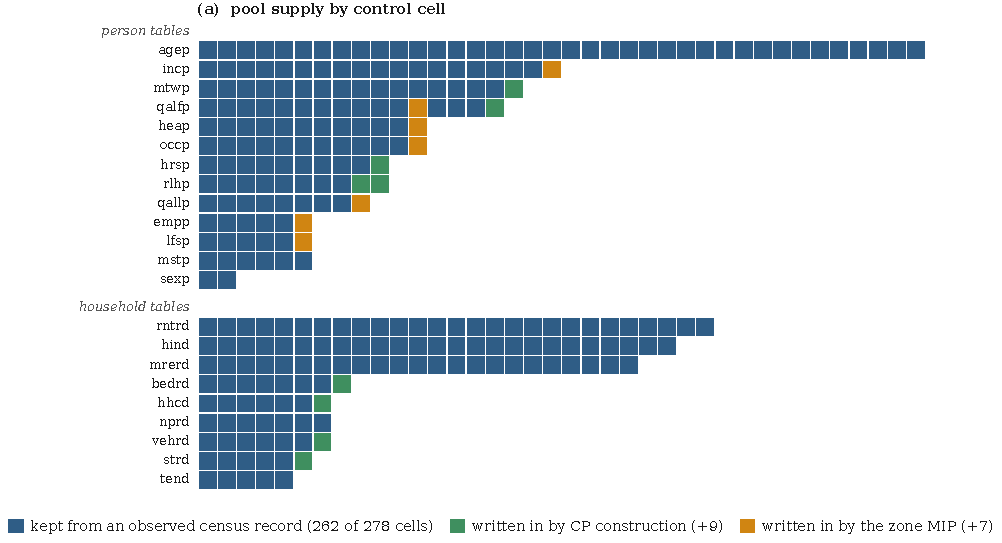
\includegraphics[width=\textwidth]{files/fig_board_pool.pdf}\\[2pt]
  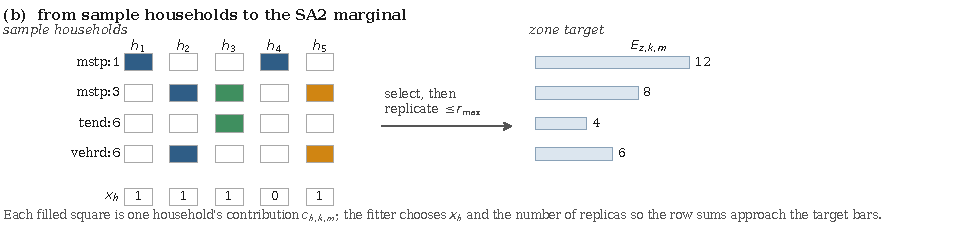
\includegraphics[width=\textwidth]{files/fig_pool_matching.pdf}
  \caption{The candidate pool as a board of control cells. \textbf{(a)} Each square is
  one category of one control table, coloured by how its cell is supplied: observed
  census records (blue), constraint-guided additions (green), and the zone's
  mixed-integer expansion (amber). \textbf{(b)} The fitting method selects
  households (\(x_h\)) and replication counts (capped at \(r_{\max}\)) so their cell
  sums \(\sum_h c_{h,k,m}x_h\) reproduce the zone's target bars \(E_{z,k,m}\).}
  \label{fig:cp_pool}
\end{figure}



\paragraph{MIP pool expansion}
\label{sec:mip_pool_expansion}
The constructed pool is feasible and cell-complete, but completeness is a
property of the pool, not of a zone: in a given zone a control-table cell
$(k,m)$ can require more records than that zone's slice of the pool can supply,
and in the limiting case no household in the slice carries the cell at all.
This is the zero-cell problem, and no weight vector or selection can repair it,
because the records needed do not exist. Expansion therefore treats the
zero-capacity case as the constraint it is, once the audit has established which
cells are in it.

\emph{What the audit measures.} For zone $z$ and control cell $(k,m)$, let
$E_{z,k,m}$ be the census target and $s_{z,k,m}$ the number of candidate records
in the zone's pool slice that carry the cell. The audit compares the target with
the \emph{attainable capacity} $r_{\max}s_{z,k,m}$, where $r_{\max}$ is the
largest number of times the zone fitter may replicate a single candidate, and
places every cell with $E_{z,k,m}>0$ in one of three states: \emph{sufficient}
if $r_{\max}s_{z,k,m}\ge E_{z,k,m}$; a \emph{partial shortfall} if
$0<r_{\max}s_{z,k,m}<E_{z,k,m}$, which replication can reach and which is
therefore left to the fitter; and \emph{zero capacity} if $s_{z,k,m}=0$, which
no weight, selection or replication can reach because the candidates are absent.
Only the third state is a pool deficiency, and only the third state is what
expansion addresses. The distinction matters for how a poor zone fit is read: a
cell in the second state is a fitting outcome, a cell in the third is a support
defect that no fitter could have avoided, and the two are reported separately
rather than pooled into one error term. \Cref{fig:mip_expansion} follows one zone
through the step, and Table~\ref{tab:cp_vs_mip} states how construction and
expansion differ.

\begin{figure}[t]
  \centering
  % =============================================================================
% fig:mip_expansion -- filling a zone's zero-capacity cells.
%
% Same board language as fig:cp_pool, one zone wide: a zone's control board has
% a positive target in a square its pool slice cannot supply at all, and no
% weight vector, selection or replication can reach it. Expansion builds
% donor x shell candidates for exactly those squares, one program per zone
% selects a handful, and the board is complete.
%
% Square states: blue = the pool slice covers the target; amber = covered but
% short; red = a positive target with no supply.
%
% Editing rules: no \\ inside a braced group; keep card text short, because the
% board is only ~2 cm tall and the cards sit beside it.
% =============================================================================
\providecolor{ForestGreen}{rgb}{0.0,0.258,0.145}
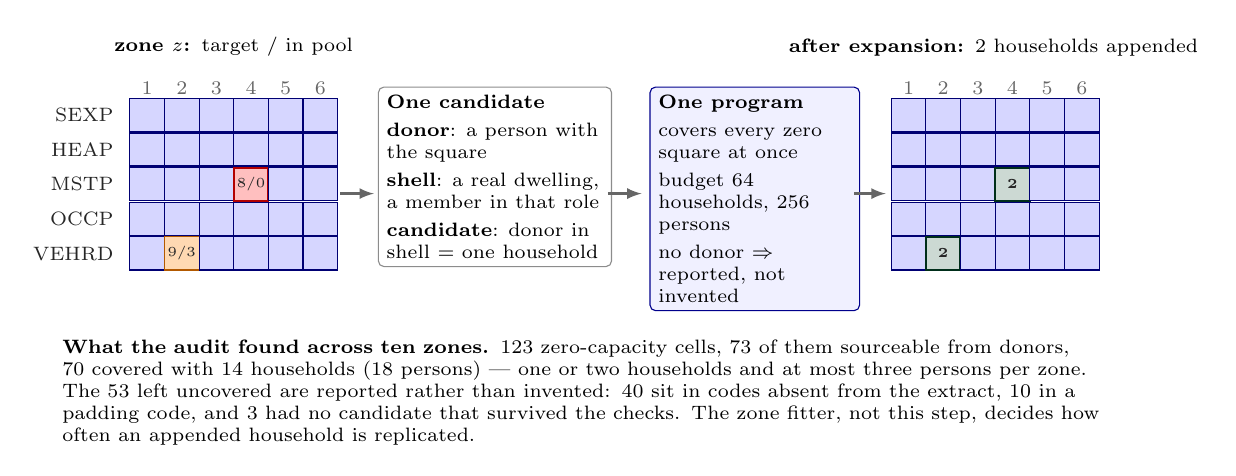
\begin{tikzpicture}[
  font=\footnotesize,
  >=latex,
  sq/.style={draw=black!50, minimum width=0.44cm, minimum height=0.42cm,
             inner sep=0pt, line width=0.4pt},
  have/.style={sq, fill=blue!16, draw=blue!45!black},
  short/.style={sq, fill=orange!30, draw=orange!70!black},
  zero/.style={sq, fill=red!25, draw=red!70!black, line width=0.8pt},
  filled/.style={sq, fill=ForestGreen!20, draw=ForestGreen!70!black, line width=0.8pt},
  hdr/.style={font=\scriptsize, text=black!60, inner sep=1pt},
  rowlab/.style={font=\scriptsize, anchor=east, text=black!85, inner sep=2pt},
  tag/.style={font=\scriptsize, text=black!75, align=center, inner sep=2pt},
  flow/.style={->, thick, draw=black!60},
  card/.style={draw=black!45, rounded corners=2pt, align=left, inner sep=3pt,
               fill=white},
  val/.style={font=\tiny, text=black!85, inner sep=0pt},
]

% ============================================================ board, zone z
\node[font=\scriptsize\bfseries, anchor=south] at (2.27,0.62)
  {zone $z$: \textnormal{target / in pool}};

\foreach \c [count=\j] in {1,...,6} {
  \node[hdr] at ({0.95+(\j-0.5)*0.44},0.34) {\c};
}

% 1 = covered, 0 = covered but short, 2 = no supply at all.
\foreach \r/\row/\name in {%
  0/{1,1,1,1,1,1}/SEXP,%
  1/{1,1,1,1,1,1}/HEAP,%
  2/{1,1,1,2,1,1}/MSTP,%
  3/{1,1,1,1,1,1}/OCCP,%
  4/{1,0,1,1,1,1}/VEHRD}%
{
  \node[rowlab] at (0.82,{-\r*0.44}) {\name};
  \foreach \d [count=\j] in \row {
    \pgfmathsetmacro{\x}{0.95+(\j-0.5)*0.44}
    \pgfmathsetmacro{\y}{-\r*0.44}
    \ifnum\d=2
      \node[zero, label={[val]center:8/0}] at (\x,\y) {};
    \else\ifnum\d=0
      \node[short, label={[val]center:9/3}] at (\x,\y) {};
    \else
      \node[have] at (\x,\y) {};
    \fi\fi
  }
}

% ======================================================== candidate for a cell
\draw[flow] (3.62,-1.00) -- (4.05,-1.00);

\node[card, anchor=north west] (cand) at (4.10,0.36) {\parbox{2.75cm}{%
  \scriptsize\raggedright
  \textbf{One candidate}\\[2pt]
  \textbf{donor}: a person with the square\\[2pt]
  \textbf{shell}: a real dwelling, a member in that role\\[2pt]
  \textbf{candidate}: donor in shell $=$ one household}};

% ================================================================ one program
\draw[flow] (7.02,-1.00) -- (7.45,-1.00);

\node[card, draw=blue!55!black, fill=blue!6, anchor=north west, name=prog]
  at (7.55,0.36)
  {\parbox{2.45cm}{\scriptsize\raggedright
  \textbf{One program}\\[2pt]
  covers every zero square at once\\[2pt]
  budget 64 households, 256 persons\\[2pt]
  no donor $\Rightarrow$ reported, not invented}};

% ==================================================================== settled
\draw[flow] (10.15,-1.00) -- (10.55,-1.00);

\node[font=\scriptsize\bfseries, anchor=south] at (11.92,0.62)
  {after expansion: \textnormal{2 households appended}};

\foreach \c [count=\j] in {1,...,6} {
  \node[hdr] at ({10.62+(\j-0.5)*0.44},0.34) {\c};
}

\foreach \r/\row/\name in {%
  0/{1,1,1,1,1,1}/SEXP,%
  1/{1,1,1,1,1,1}/HEAP,%
  2/{1,1,1,3,1,1}/MSTP,%
  3/{1,1,1,1,1,1}/OCCP,%
  4/{1,3,1,1,1,1}/VEHRD}%
{
  \foreach \d [count=\j] in \row {
    \pgfmathsetmacro{\x}{10.62+(\j-0.5)*0.44}
    \pgfmathsetmacro{\y}{-\r*0.44}
    \ifnum\d=3
      \node[filled, label={[val]center:\textbf{2}}] at (\x,\y) {};
    \else
      \node[have] at (\x,\y) {};
    \fi
  }
}

% ================================================================ audit line
% Anchored below the tallest card rather than at a fixed y, so the note cannot
% collide with the card text when the wording changes.
\node[anchor=north west, align=left, text width=13.2cm, font=\scriptsize,
      inner sep=1pt] at ($(prog.south west)+(-7.50,-0.32)$)
  {\textbf{What the audit found across ten zones.} 123 zero-capacity cells, 73 of
   them sourceable from donors, 70 covered with 14 households (18 persons) --- one
   or two households and at most three persons per zone. The 53 left uncovered are
   reported rather than invented: 40 sit in codes absent from the extract, 10 in a
   padding code, and 3 had no candidate that survived the checks. The zone fitter,
   not this step, decides how often an appended household is replicated.};

\end{tikzpicture}

  \caption{How a zone's zero-capacity cells are filled. For each zone the audit compares
  every positive-target cell with the supply in that zone's pool slice; on the board, a
  filled square is a cell the slice covers, an amber square one it covers only partly, and
  a red square one it cannot supply at all. A square with no supply cannot be reached by
  any weight vector, selection or replication. Each such cell
  receives a candidate: a real donor who carries the cell, written into a real shell
  dwelling from the same region that already has a member in the donor's role, so the
  dwelling and family terms stay observed rather than invented. One program per zone then
  selects a small set of candidates covering all zero cells at once, and the selected
  households are appended to the pool with fresh identifiers. Coverage is soft: a cell with
  no donor anywhere is reported by the audit rather than synthesised, and the zone fitter
  (IPU, SA or MIP), not this step, decides how often an appended household is replicated.}
  \label{fig:mip_expansion}
\end{figure}


\begin{table}[h!]
\centering
\caption{The two pool-side programs answer different questions and are not
substitutes. Construction makes the pool complete over the modelled attributes for
every zone at once; expansion repairs the cells a single zone's slice cannot supply.
Neither stage allocates records to zones, which is why both are followed by a fitter.}
\label{tab:cp_vs_mip}
\footnotesize
\setlength{\tabcolsep}{5pt}
\begin{tabular}{@{}>{\raggedright\arraybackslash}p{1.7cm}
                 >{\raggedright\arraybackslash}p{5.6cm}
                 >{\raggedright\arraybackslash}p{6.3cm}@{}}
\toprule
 & \textbf{CP pool construction} & \textbf{MIP pool expansion} \\
\midrule
Question & Can every rule-feasible cell be represented in the pool at all? &
Which cells can this zone's slice not supply, and which households can fill them? \\
Scope & The whole census, all zones at once, all 19 control tables &
One zone, and only the cells the audit places in the zero-capacity state \\
Decision & Which category each modelled attribute takes, given a household shell and the
observed conditional distributions & Which candidates enter a small added set, one binary
per candidate, against all marginal tables at once \\
Guarantee & Every emitted record satisfies $\mathcal{R}$, and the pool is cell-complete
over the modelled attributes & Every added household satisfies $\mathcal{R}$, and every
sourceable zero cell receives at least one candidate \\
Does not & Use zone targets, match any zone total, or decide replication & Close the
zone's full deficit, fit its totals, or decide how often a candidate is used \\
Cost & 27.1 minutes and 5.0\,GB for the whole pool, once & About 100 seconds per zone,
and only where zero cells exist \\
Result here & 1{,}404{,}801 persons, no rule violations & 14 households (18 persons)
across the ten audit zones \\
\bottomrule
\end{tabular}
\end{table}

\emph{Candidate construction.} For a zone $z$ let $\mathcal{Z}_z^0$ be the set of
control cells with a positive census target and zero attainable capacity in the
zone's candidate pool. For each such cell the module draws donor records from the
census microdata that carry the cell, pairs each donor member profile with a real
shell household from the same \texttt{REGUCP} that has a member in the donor's
\texttt{RLHP} role, and writes the donor profile into that slot. If the donor
profile conflicts with the shell's dwelling terms or with the rule set
$\mathcal{R}$, a small completion program finds the closest feasible profile,
\begin{equation}
\min_{y}\;\sum_{a}\bigl(1-y_{a,\tau(a)}\bigr)
\quad\text{s.t.}\quad
\sum_{c} y_{a,c}=1,\;\;
y_{a_1,c_1}+y_{a_2,c_2}\le 1 \;\;\forall\,(a_1,c_1,a_2,c_2)\in\mathcal{C},
\label{eq:mip_repair}
\end{equation}
where $\tau(a)$ is the donor's code for attribute $a$ and $\mathcal{C}$ is the
set of forbidden category pairs obtained by evaluating the shared rule set over
every attribute domain mesh (2{,}027 cuts in the ten-zone development audit).
Equation~\eqref{eq:mip_repair} is a \emph{candidate repair}, not the pool
objective: it preserves a real donor profile wherever the hard rules allow, and
it is solved separately for each candidate before any selection. The
household-level fields are fixed to the shell, so every candidate remains atomic
and family-coherent; candidates that fail the shared
rule checks are discarded, never patched. For attributes outside
the person-level model (e.g.\ \texttt{tend}, \texttt{typp}, \texttt{indp},
\texttt{stup}, \texttt{assnp}), a person-level repair is not available, so the
module falls back to a whole real donor household copied verbatim; the observed
household is feasible by construction.

\emph{Joint-marginal selection.} The candidates are then selected together, not
cell by cell. Let $\mathcal{J}_z$ index the candidate households,
$x_j\in\{0,1\}$ indicate selection, and $s_j$ be the number of persons in
candidate $j$. For a control cell $(k,m)$, let $a_{j,k,m}$ be the candidate's
contribution---the number of its members in the cell for a person-level table, or
one if the household sits in the cell for a household-level table---and let
$u_{j,k}=s_j$ for a person-level table and $u_{j,k}=1$ for a household-level
table. With the zone target $E_{z,k,m}$ and target share
\begin{equation}
q_{k,m}=\frac{E_{z,k,m}}{\sum_{m'\in\mathcal{M}_k}E_{z,k,m'}},
\label{eq:mip_share}
\end{equation}
the selection program is
\begin{equation}
\begin{aligned}
\min_{x,e,d}\quad &
\lambda_0\sum_{c\in\mathcal{Z}_z^0} e_c
\;+\;\sum_{k\in\mathcal{K}}\sum_{m\in\mathcal{M}_k} w_{k,m}\,d_{k,m}
\;+\;\lambda_1\sum_{j\in\mathcal{J}_z} x_j \\
\text{s.t.}\quad &
\sum_{j\in\mathcal{J}_z} a_{j,c}\,x_j+e_c\ge 1,
&& c\in\mathcal{Z}_z^0,\\
& d_{k,m}\ge \sum_{j\in\mathcal{J}_z}
  \bigl(a_{j,k,m}-q_{k,m}u_{j,k}\bigr)x_j,
&& k\in\mathcal{K},\,m\in\mathcal{M}_k,\\
& d_{k,m}\ge -\sum_{j\in\mathcal{J}_z}
  \bigl(a_{j,k,m}-q_{k,m}u_{j,k}\bigr)x_j,
&& k\in\mathcal{K},\,m\in\mathcal{M}_k,\\
& \sum_{j\in\mathcal{J}_z}x_j\le K_z,\qquad
  \sum_{j\in\mathcal{J}_z}s_jx_j\le P_z^{\mathrm{add}},\\
& \sum_{j\in\mathcal{J}_z(h)}x_j\le 1,
&& h\in\mathcal{H}_z,\\
& x_j\in\{0,1\},\quad e_c\ge 0,\quad d_{k,m}\ge 0.
\end{aligned}
\label{eq:mip_joint}
\end{equation}
Here $w_{k,m}=1/(|\mathcal{M}_k|\max(E_{z,k,m},1))$ gives every control table
equal weight and prevents large person tables from dominating; the
implementation divides $w$ by its maximum, a positive rescaling that does not
change the argmin. The released defaults are $\lambda_0=10^5$ and
$\lambda_1=10^{-2}$. With the default 256-person budget the whole marginal term
is below about $2.6\times10^4$, so covering one zero cell is worth more than
any marginal improvement the added set can buy. Coverage is still soft: an
unsourceable cell cannot make the program infeasible, and a cell can be left
uncovered when the budget or the candidate menu makes coverage impossible.
$K_z$ and $P_z^{\mathrm{add}}$ are small budgets (defaults: 64 households and
256 persons per zone), not the zone's population. The constraint over
$\mathcal{J}_z(h)\subseteq\mathcal{J}_z$ permits at most one transplant per
shell household.

The important difference from a per-cell objective is that
\eqref{eq:mip_joint} uses \emph{one} selection vector $x$ for \emph{all} control
tables. The deviations $d_{k,m}$ are therefore not independent cell repairs:
they measure how far the selected agents' aggregate profile is from the zone's
total marginal composition, table by table, and the solver must trade those
deviations against one another and against coverage. A set of records that fills
every zero cell but distorts the income or tenure shares is penalised; a set that
matches the shares but leaves a zero cell uncovered is penalised more heavily
through $\lambda_0$. This is a joint fit over the marginal tables, not a fit to
the full joint distribution: one selection vector must satisfy every table
simultaneously, while the joint distribution over attribute combinations is the
object of the zone fitter, not of the small pool-expansion program. The
coverage constraints are soft ($e_c$) precisely so that an unsourceable
cell---a structural zero, a padding code, or a cell with no donor anywhere---does
not make the program infeasible; it is reported instead.

The model is deliberately \emph{not} required to close the measured shortfall.
The deficit in a zone is often tens of thousands of persons, while the candidate
pool is a 5\% microsample and the added set is a few dozen households. Requiring
$\sum_j a_{j,k,m}x_j\ge E_{z,k,m}$ for every cell would either be infeasible or
force the pool to replicate the census many times over, which is the fitter's
job, not the pool's. What the expansion asks for is weaker and sufficient:
\emph{every zero cell for which a candidate exists should receive at least one
feasible candidate}, and the added candidates should jointly resemble the zone's
marginal totals. Because coverage is soft, a cell can still be left uncovered
when the budget or the candidate menu makes coverage impossible; such cells are
reported rather than silently dropped. The zone fit that follows decides which
candidates are actually used.

The module reports, per zone, the number of zero-capacity cells, how many are
covered, the selected household and person counts, the weighted joint-marginal
deviation, and the uncovered cells; the candidate-skip reasons are aggregated
over the run.

\emph{Development audit.} A ten-zone audit at the released defaults found 123
zero-capacity cells among 146 deficient cells (the other 23 were partial
shortfalls left to the zone fitter). The module generated donor--shell
candidates for 70 of the 73 sourceable zero cells and the joint selection
covered all 70, using 14 households (18 person rows) in total---one or two
households and at most three persons per zone, far inside the 64-household and
256-person budgets. All ten selection programs solved to optimality, and every
selected row passed the 11 shared rule checks. The 53 cells
left uncovered were 40 cells in four control codes absent from the census
extract, 10 \texttt{tend:6} padding cells, and three \texttt{tenlld:11} cases where no
donor--shell candidate survived the household and rule checks. The weighted
joint-marginal deviation of the added set was 0.239--1.622 per zone (median
0.406), and its unweighted mean absolute cell deviation was 0.126--0.280. These
are deviations of the added set, not of the fitted zone population; the audit
establishes that the mechanism can fill the sourceable zero cells with a small
number of feasible records, not that it closes the zone's full deficit.
Appendix~\ref{sec:pool_expansion_audit} gives the per-zone table and the
interpretation of the residual cells.
%% Audit source: outputs/full10_joint_report.json and
%% outputs/full10_joint_audit.log (10 zones, joint mode, released defaults;
%% 1,013.5 s).



\subsection*{Results structure}
The results are reported in four parts, each answering one question. Pool
construction quality asks whether the constructed pool resembles the
population it is built from. Coverage quality asks whether the pool supplies
every positive-target control cell. Fit quality asks whether the fitted
population reproduces the 19 control tables. Joint-distribution quality asks
whether the fitted population preserves associations and avoids duplication.
Pool and coverage metrics are reported before fit metrics, and fit metrics are
not used to judge the pool.

\subsection{Pool construction quality}
\label{sec:pool_construction}

The candidate pool is built by \emph{feasibility-constrained construction} from the census rather than by sampling a fitted joint model: the constraint-programming (CP) feasible pool and its mixed-integer expansion are described in \cref{sec:cp} and \cref{sec:mip_expansion_formulation}. This subsection describes the household composition those records carry and how
close the constructed pool sits to the census marginal before fitting.

\subsubsection{Household composition of the pool}
\label{sec:households}
Households are the atomic unit throughout the synthesis process. Every person
record belongs to a household when it enters the candidate pool, and no stage
reconstructs households from independent individuals. The fitting methods
operate on complete households, adding, removing, weighting, or swapping whole
households rather than assembling new ones from person records. All households
in the pool originate from observed census households; constructed candidates
are donor--shell grafts into real census shells, and every candidate is checked
against the shared consistency rules before entering the pool. Candidates that
fail validation are discarded rather than repaired after construction. The pool
therefore carries household-size and relationship structures that originate
from census households, not from a separate grouping step.


\cref{fig:pool_tvd_by_size} isolates the pool stage: it is the mean TVD between
each pool and the census marginal before any fitting. The raw SA4 slice is
slightly closer than the CP pool and the expanded pool in every size quintile,
and all three distances are lower in the larger quintiles, with a local rise at
Q3. Construction and expansion therefore buy feasibility, household coherence
and support for uncovered cells rather than marginal proximity; adding the
constructed carriers recovers a small net gain (0.1060 to 0.1053 on the
19-table mean), and the fitting method closes the rest of the gap. The pool-target
comparison uses all 19 control tables. The census control files store category
labels, while the pool records store integer codes; the crosswalk in
\texttt{CensusRecordImporter.define\_mapping()} maps each label to the code the
fitter uses, and it applies to \texttt{nprd} (persons per dwelling) and
\texttt{strd} (dwelling structure) exactly as it does to the other tables, so no
table is excluded. The 19-table mean is 0.106 for the raw slice, 0.107 for the
CP pool and 0.107 for the expanded pool.

\begin{figure}[H]
\centering
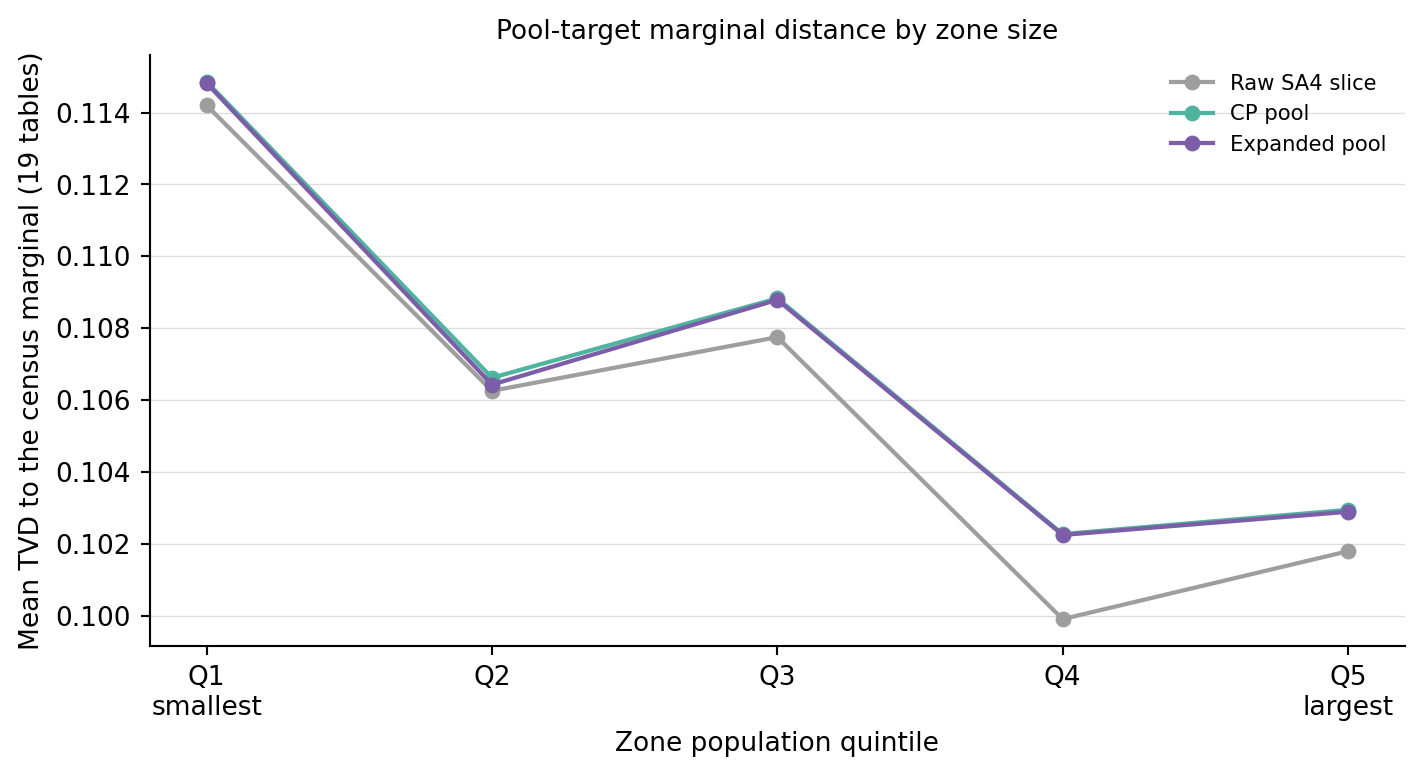
\includegraphics[width=0.78\textwidth]{fig_pool_tvd_by_size.png}
\caption{Mean total-variation distance between each pool stage and the census
marginal, averaged over all 19 control tables, by zone population quintile (Q1
smallest to Q5 largest). The pools are compared before fitting and lower is
better.}
\label{fig:pool_tvd_by_size}
\end{figure}

\Cref{fig:pool_stage_heatmap} gives the cohort-level view across all 19
control tables: it expresses each stage's TVD as a percentage of the maximum
TVD attainable against the same census marginal, so tables with different
category counts and minimum shares are comparable. A value of 0\% is a perfect
fit and 100\% is the worst possible fit; lower is better. The side columns show
where the carrier stage has real work to do: relationship in household and
student status carry 6.8\% and 5.3\% of their target mass in zero-capacity
cells, whereas field of study has more zero cells (681) but only 0.3\% of its
target mass. That is why the carrier column moves the first two tables more
than the last. The donor-balanced column is the balance track: whole census
households are scored by their net reduction in the final weighted deviation
and added iteratively in 5\% batches up to a 100\% person budget. It lowers the
relative TVD for every table, with the largest gains in highest education
(11.7\% to 8.6\%), field of study (6.9\% to 3.7\%), occupation (6.6\% to
3.3\%), qualification level (6.9\% to 3.0\%) and hours worked (5.4\% to 2.7\%).
The cohort mean falls from 0.1053 to 0.0816. Household income, relationship in
household and dwelling structure remain higher because the observed donor pool
is itself skewed; the fit-time dwelling-structure band shift addresses the last
of these.

\begin{figure}[H]
\centering
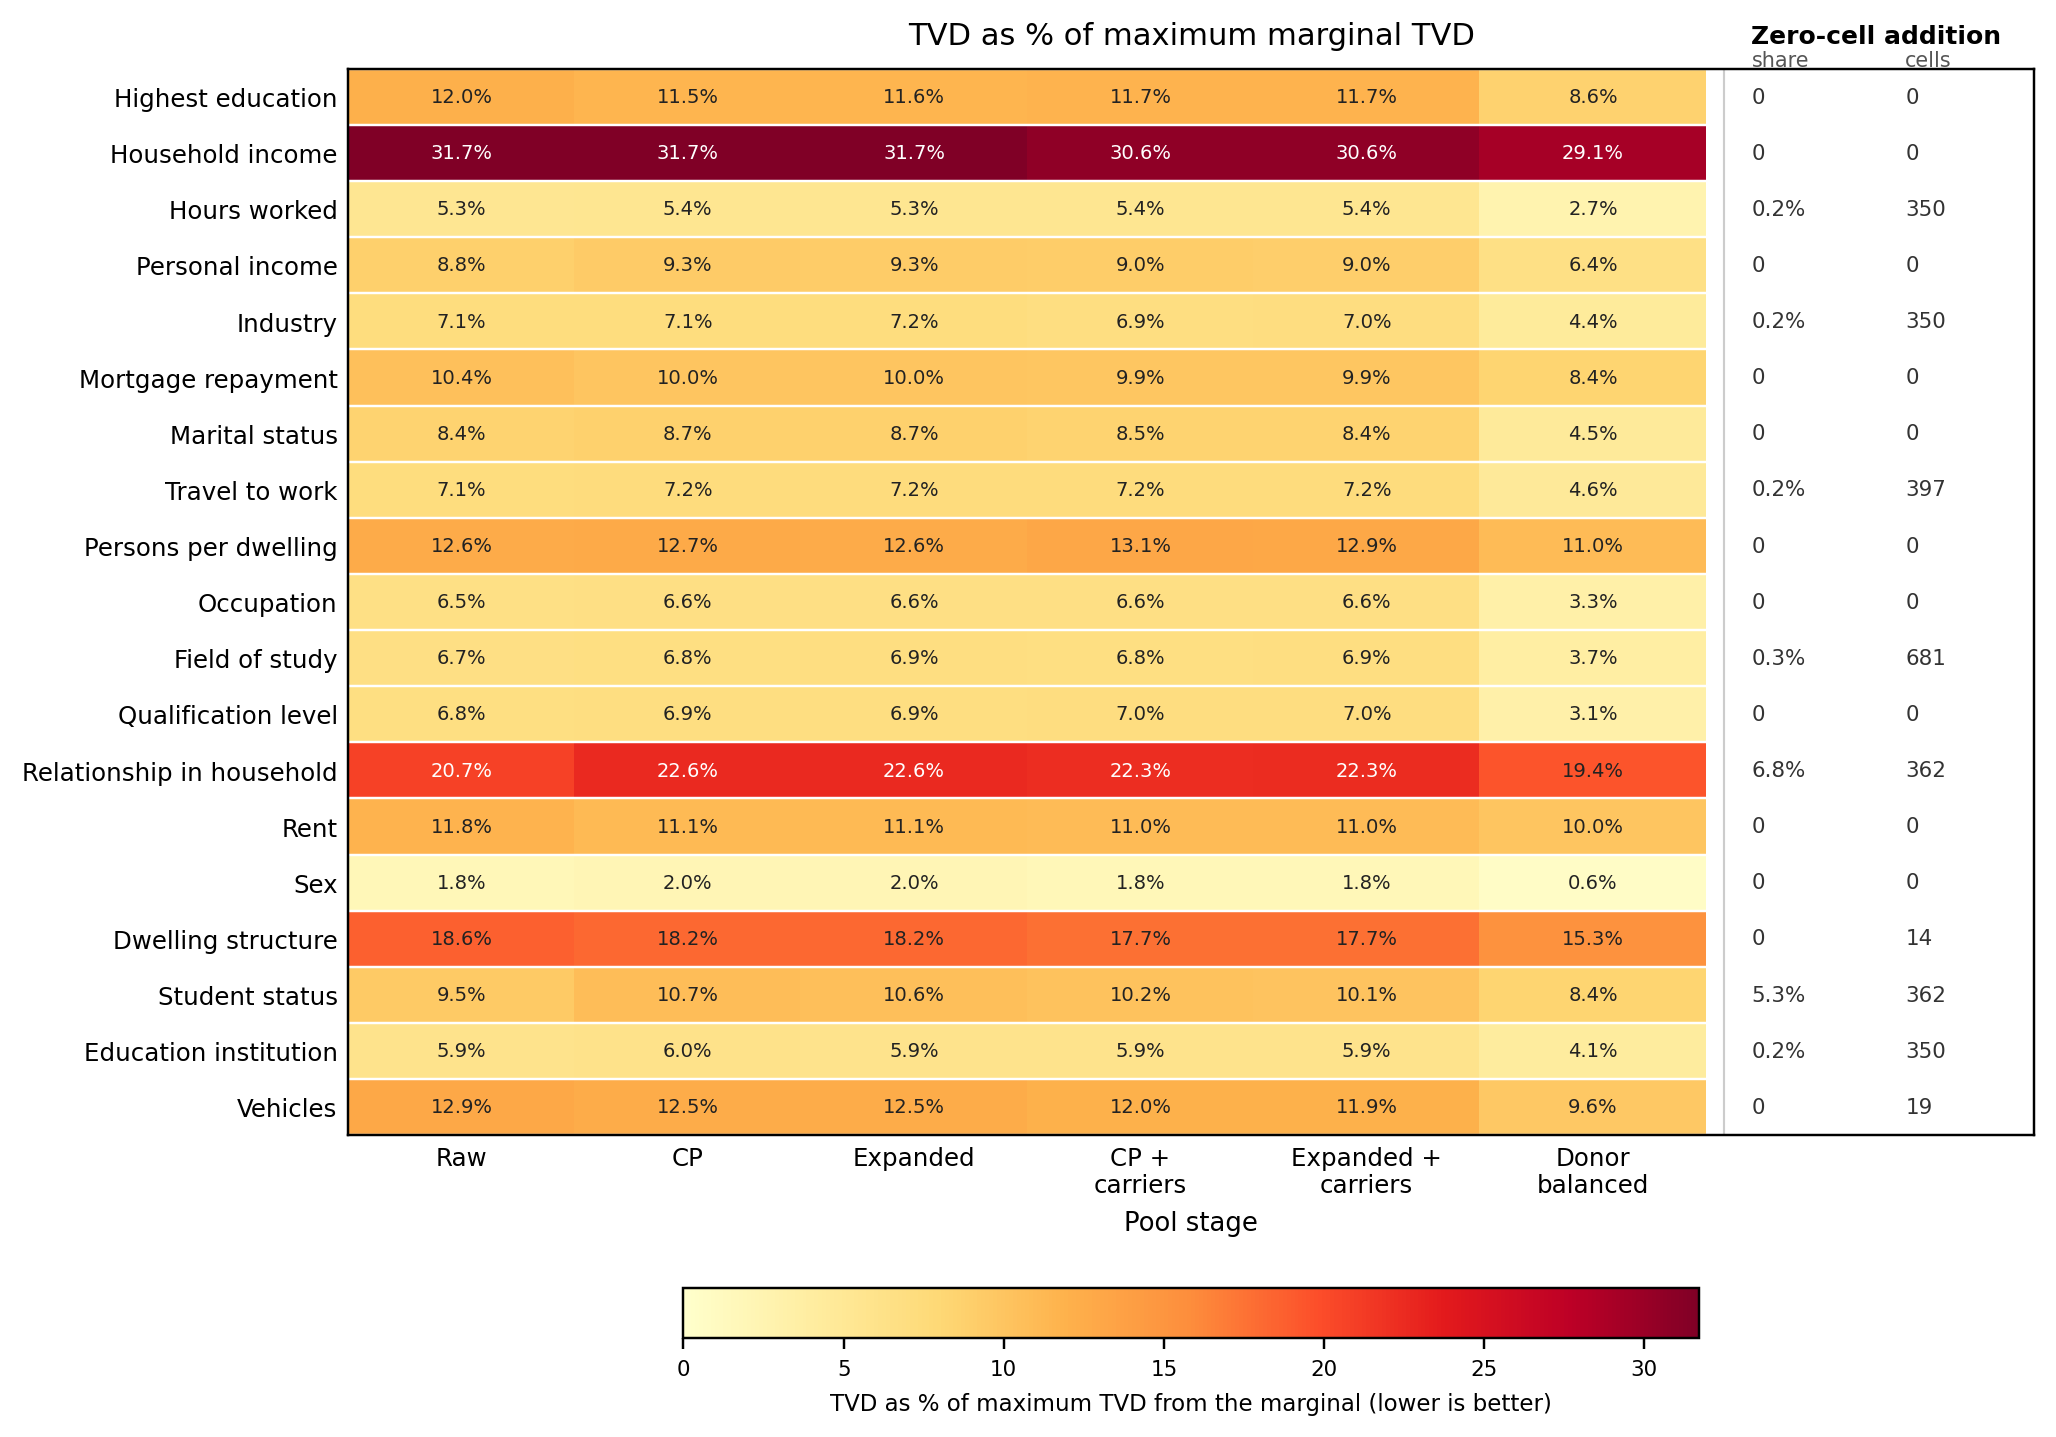
\includegraphics[width=\textwidth]{fig_pool_stage_heatmap.png}
\caption{Mean total-variation distance between each pool stage and the census
marginal, by control table, averaged over the 362 fitted zones and shown for
all 19 control tables. Cell values are the stage TVD as a percentage of the
maximum TVD attainable against that table's census marginal,
$100\times \mathrm{TVD}/(1-\min_m q_{z,k,m})$, averaged over zones: 0\% is a
perfect fit and 100\% is the worst possible fit for that marginal. Lower is
better. The right-hand columns give the share of the table's census target that
sits in zero-capacity cells---the part the carrier stage has to add rather than
reweight---and the number of such cells. The final column is the donor-balanced
pool: whole census households scored by their net reduction in the final
weighted marginal deviation and added iteratively in 5\% batches up to a 100\%
person budget. It lowers the relative TVD for every table, with the largest
gains in highest education, field of study, occupation, qualification level and
hours worked.}
\label{fig:pool_stage_heatmap}
\end{figure}

\Cref{fig:pool_stage_raw_delta} rescales the same values to the raw
microdata, so the total change from the raw category is visible for every table.

\begin{figure}[H]
\centering
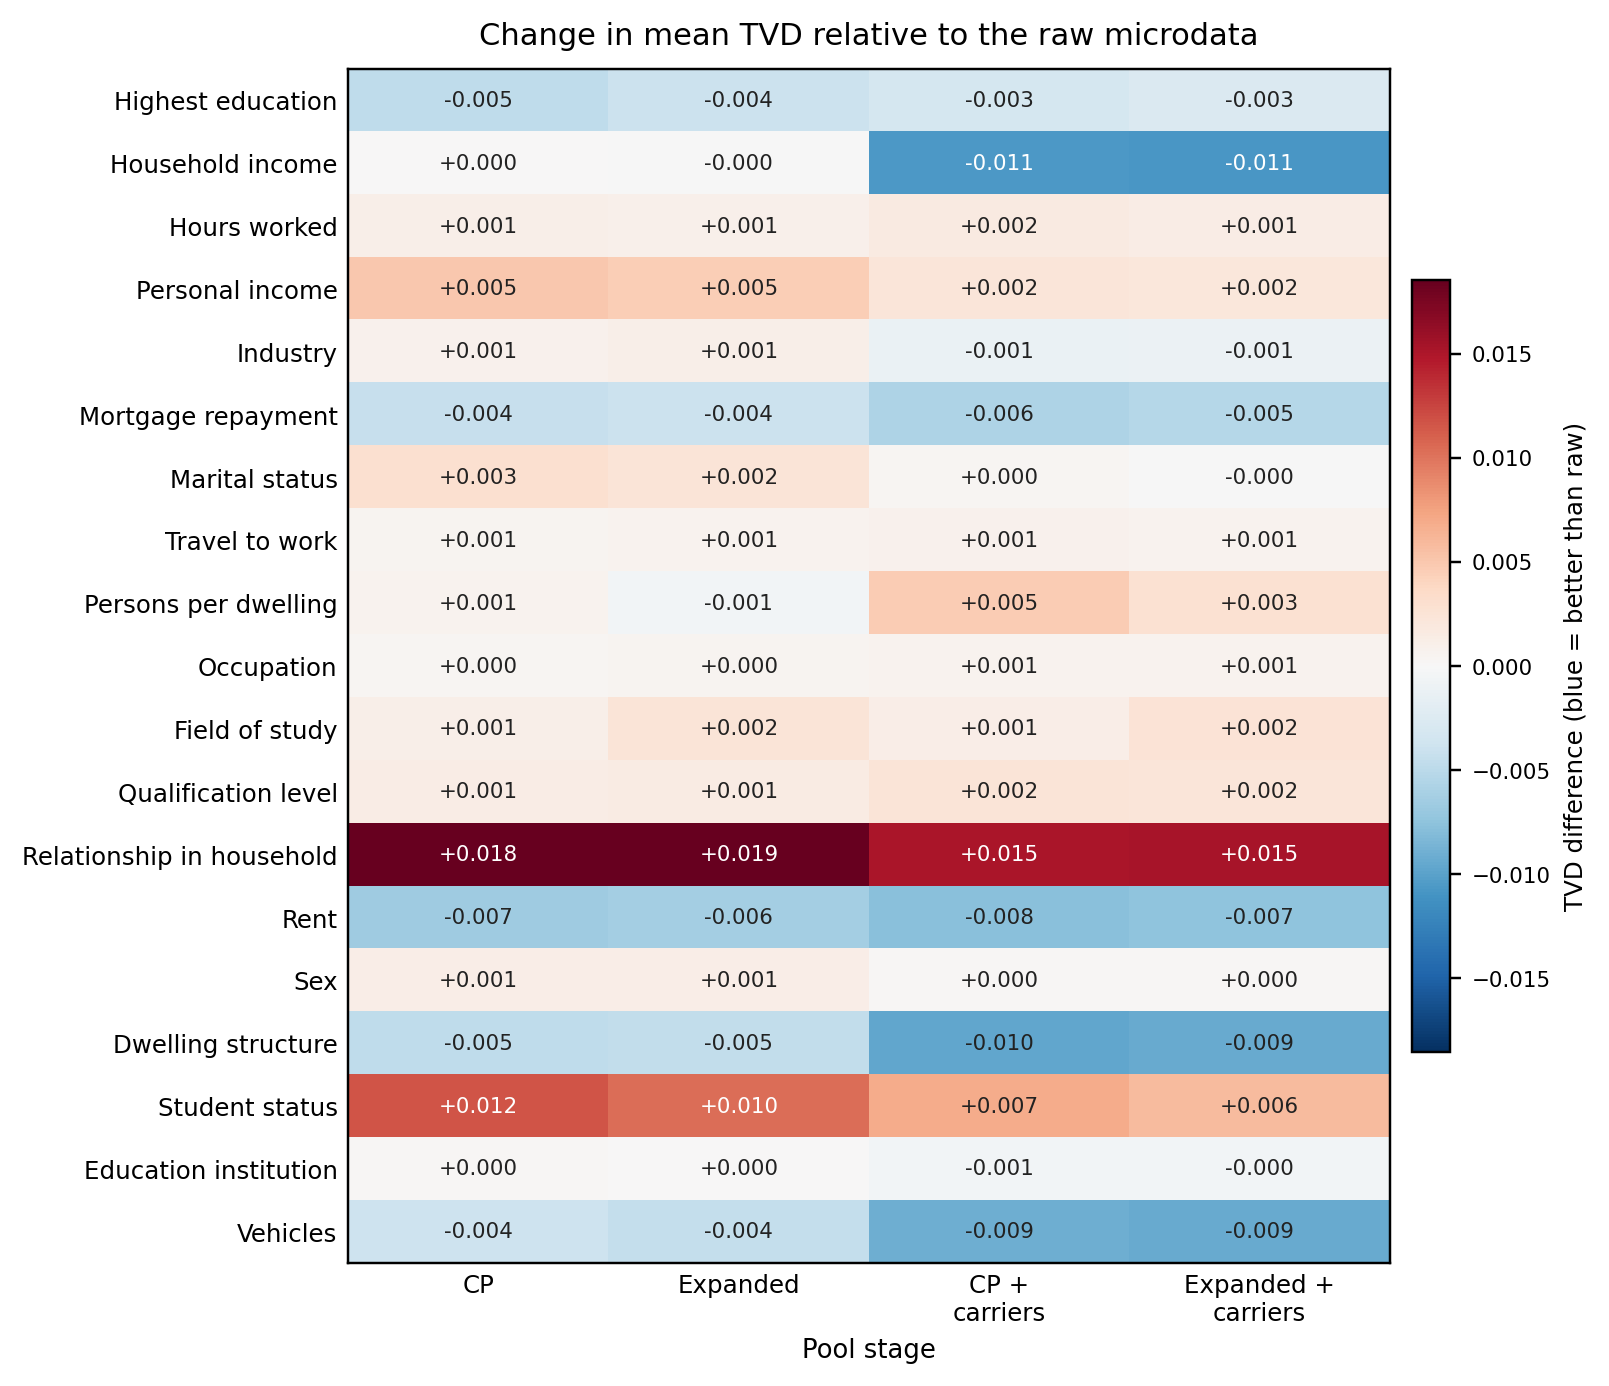
\includegraphics[width=0.78\textwidth]{fig_pool_stage_raw_delta.png}
\caption{Change in mean TVD relative to the raw microdata, by control table and
pool stage, for all 19 control tables. Blue = better than raw, red = worse. The
final column is the pool with constructed carriers.}
\label{fig:pool_stage_raw_delta}
\end{figure}

\Cref{tab:zone_marginal} and
\cref{fig:zone_progression_all,fig:pool_progression_by_size} give the category
detail behind the cohort summary. \Cref{fig:zone_progression_all} traces the
mean per-zone category gap from the raw slice through the CP and expanded pools
to the fitted population. Expansion is coverage-driven rather than a
marginal-rebalancing step, so some pool-stage gaps widen; the fitted column is
where the fitting method pulls the marginals back.
\Cref{fig:pool_progression_by_size} shows the same path for five representative
zones and makes the rebalancing visible at the zone level. The constructed
pools are closer for most small categories, while the large categories are
already within the $\pm0.2$ pp band in the raw slice.

\subsection{Coverage quality}
\label{sec:pool_growth}
\cref{tab:pool_growth} isolates the effect of pool construction independently of any fitted solution. Relative to the raw extract, CP construction increases the number of persons, households, and distinct tuples. The observed-donor expansion contributes comparatively few additional persons because it is driven by sourceable coverage deficits rather than pool size, and introduces only a modest number of new tuples. The second stage adds many more, because it constructs a carrier for every deficit cell rather than only the cells a census donor can source. The resulting pool is therefore richer in the dimension that matters downstream, namely support for previously uncovered control cells, without changing any fitting targets. The ``Covered at $\nu_c$'' column reports the sample-zero cells supplied by expansion. For a cell with census target \(E_{z,k,m}\), the carrier requirement \[ \nu_c=\left\lceil \frac{E_{z,k,m}}{r_{\max}} \right\rceil \] is the minimum number of carrier households needed to reach the target under the replication cap \(r_{\max}\). Expansion writes \(\nu_c\) carrier households for every sourceable sample-zero cell, covering 383 of the 2{,}890 such cells; the second stage constructs carriers for the remaining 2{,}507, so the final pool covers all 2{,}890. The residual column is 2{,}890 in the CP pool, 2{,}507 after donor expansion, and 0 after carrier construction.
\begin{table}[H]
\centering
\caption{Person and household counts.}
\label{tab:pool_growth}
\footnotesize
\setlength{\tabcolsep}{4pt}
\begin{tabular}{@{}lrrrrrr@{}}
\toprule
Stage & Persons & Households & Distinct tuples & Zero-capacity & Covered at \(\nu_c\) & Residual zero cells \\
\midrule
Raw census        & 1{,}252{,}479 & 488{,}717 & 1{,}028{,}656 & n/a & n/a & n/a \\
CP feasible pool  & 1{,}396{,}342 & 549{,}699 & 1{,}165{,}391 & 2{,}890 & 0 & 2{,}890 \\
CP + donor expansion & 1{,}399{,}373 & 551{,}235 & 1{,}165{,}540 & 2{,}890 & 383 & 2{,}507 \\
CP + donor + carriers & 1{,}741{,}952 & 768{,}581 & 1{,}179{,}772 & 2{,}890 & 2{,}890 & 0 \\
\bottomrule
\end{tabular}
\end{table}

{\footnotesize\textit{Note:} persons and households are pool-level counts. The
zero-capacity, coverage and residual columns are for the 362-zone fitted cohort;
the final row adds the full 367-zone carrier set (217{,}346 households,
342{,}579 persons). The 362-zone carrier set is 216{,}196 households and
340{,}927 persons.}
\Cref{tab:mip_objective} separates the support program's objective from its
coverage outcome.
\begin{table}[H]
\centering
\caption{Objective terms and coverage outcome of the support program on the
362-zone cohort. The reported run uses
$\lambda_0\sum_c e_c+\lambda_c\sum_{k,m}w_{k,m}d_{k,m}+\lambda_1\sum_j y_j$
with $\lambda_0=10^5$, $\lambda_c=1$ and $\lambda_1=10^{-2}$; the lower block
reports coverage.}
\label{tab:mip_objective}
\footnotesize
\setlength{\tabcolsep}{4pt}
\begin{tabular}{@{}lr@{}}
\toprule
Term or outcome & Value \\
\midrule
Coverage penalty $\lambda_0\sum_c e_c$ & 1{,}394{,}200{,}000 \\
Marginal deviation $\sum w d$ & 81.66 \\
Parsimony $\lambda_1\sum_j y_j$ & 3.87 \\
Objective, sum over zones & 1{,}394{,}200{,}086 \\
Objective per zone, median (range) & 3{,}400{,}000 (0--15{,}200{,}000) \\
\midrule
\multicolumn{2}{@{}l}{\emph{Coverage outcome}} \\
Zero-capacity cells & 2{,}890 \\
Covered at $\nu_c$ (zero cells) & 383 (13.3\%) \\
Residual (uncovered zero cells) & 2{,}507 \\
Coverage set & 387 households (768 persons) \\
Whole-build addition & 1{,}536 households (3{,}031 persons) \\
\bottomrule
\end{tabular}
\end{table}

{\footnotesize\textit{Note:} a zero-capacity cell has a positive census target
$E_{z,k,m}>0$ and no carrier in the zone's CP pool. ``Covered at $\nu_c$'' means
the expanded pool supplies at least
$\nu_c=\lceil E_{z,k,m}/r_{\max}\rceil$ carriers for the cell. ``Residual'' is
the count of zero-capacity cells that still have no carrier after expansion; it
is a support gap reported by the audit, not a cell the fitting method failed to
match, and it excludes structural zeros ($E_{z,k,m}=0$), which are fixed at zero
by construction. The coverage set is the subset of added households selected to
certify coverage; the whole-build addition is every donor--shell household
appended to the pool.}

The support program is only the first expansion stage. Of its 2{,}507 residual
cells, a subset cannot be sourced from any census donor at all --- the control
category has no ancestor in the microdata, so no donor--shell construction
exists for it. A second, deficit-driven stage constructs those carriers
directly, patching the target attribute onto a rule-valid household from the
zone's SA4 slice and tagging the result to the SA2. \Cref{tab:expansion_drivers}
lists the largest cells it supplies. The two stages are separate in the
pipeline: the first restores coverage the census can support, the second
supplies the categories it cannot, and the fitted arms are labelled accordingly
in \cref{tab:strategy_roles}. Together they cover all 2{,}890 zero-capacity
cells: 383 from donor--shell expansion and 2{,}507 from constructed carriers.
Expansion adds candidates only where the pool lacks a carrier, so the constructed
set is sized by the deficit rather than by a fixed sample.

\input{files/zone_marginal_progression.tex}

\begin{figure}[H]
\centering
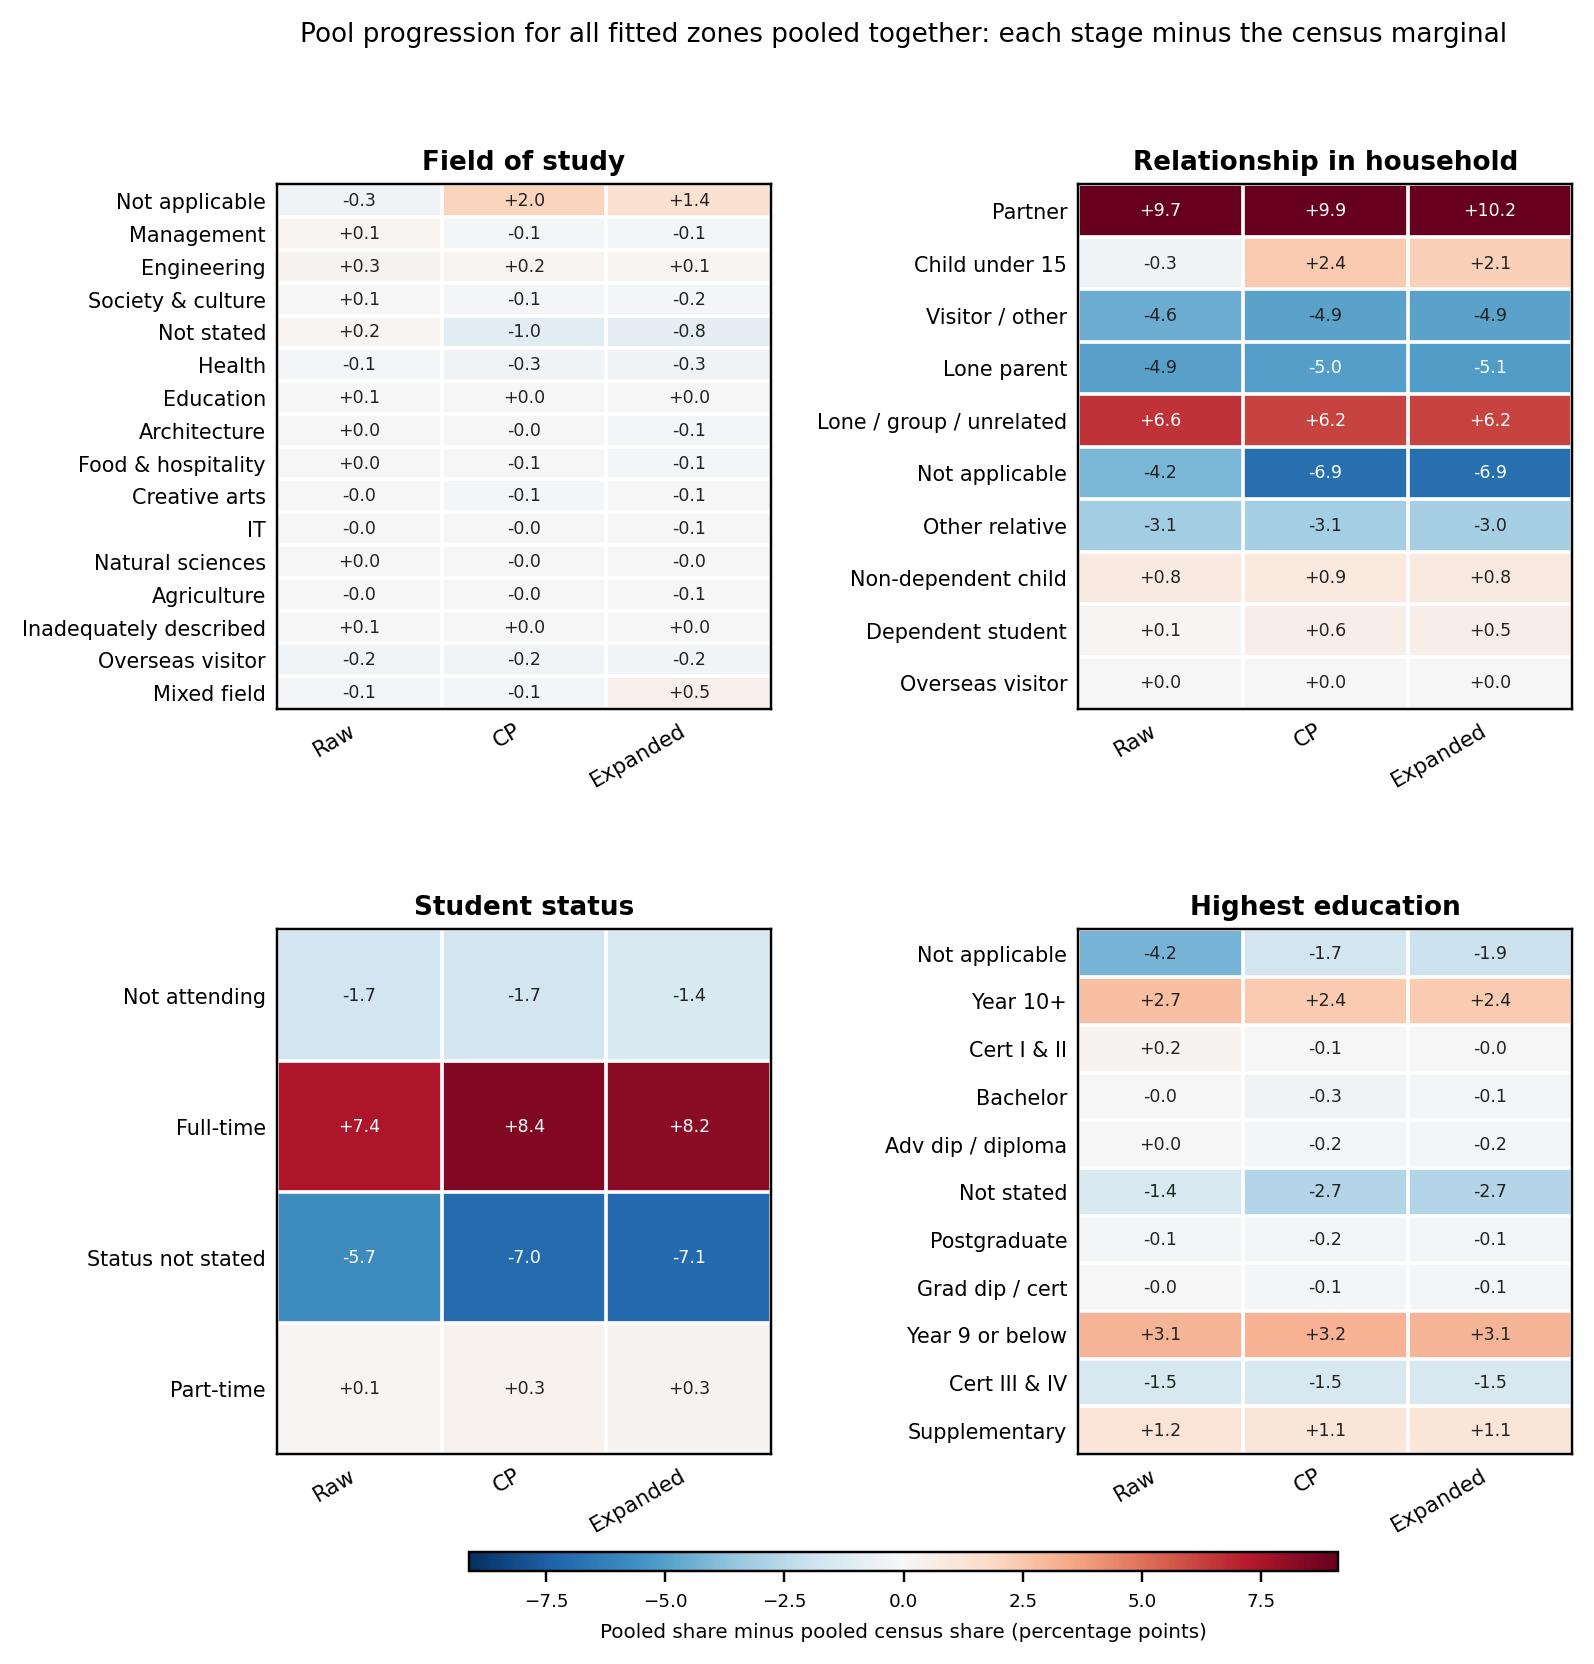
\includegraphics[width=\textwidth]{fig_zone_progression_all.png}
\caption{Mean per-zone progression from the raw slice to the fitted population
across all 362 fitted zones and four control tables. Each row is a category and
each column a stage---raw SA4 slice, CP pool, expanded pool and fitted
population. The cell is the mean, over the 362 zones, of the zone's stage share
minus the zone's census share in percentage points. Blue = close to the census
share, red = a large gap in either direction; the sign is printed in each cell
(positive = over-representation, negative = under-representation). The fitted
column is the expanded population after carriers and zone fitting.}
\label{fig:zone_progression_all}
\end{figure}

\begin{figure}[H]
\centering
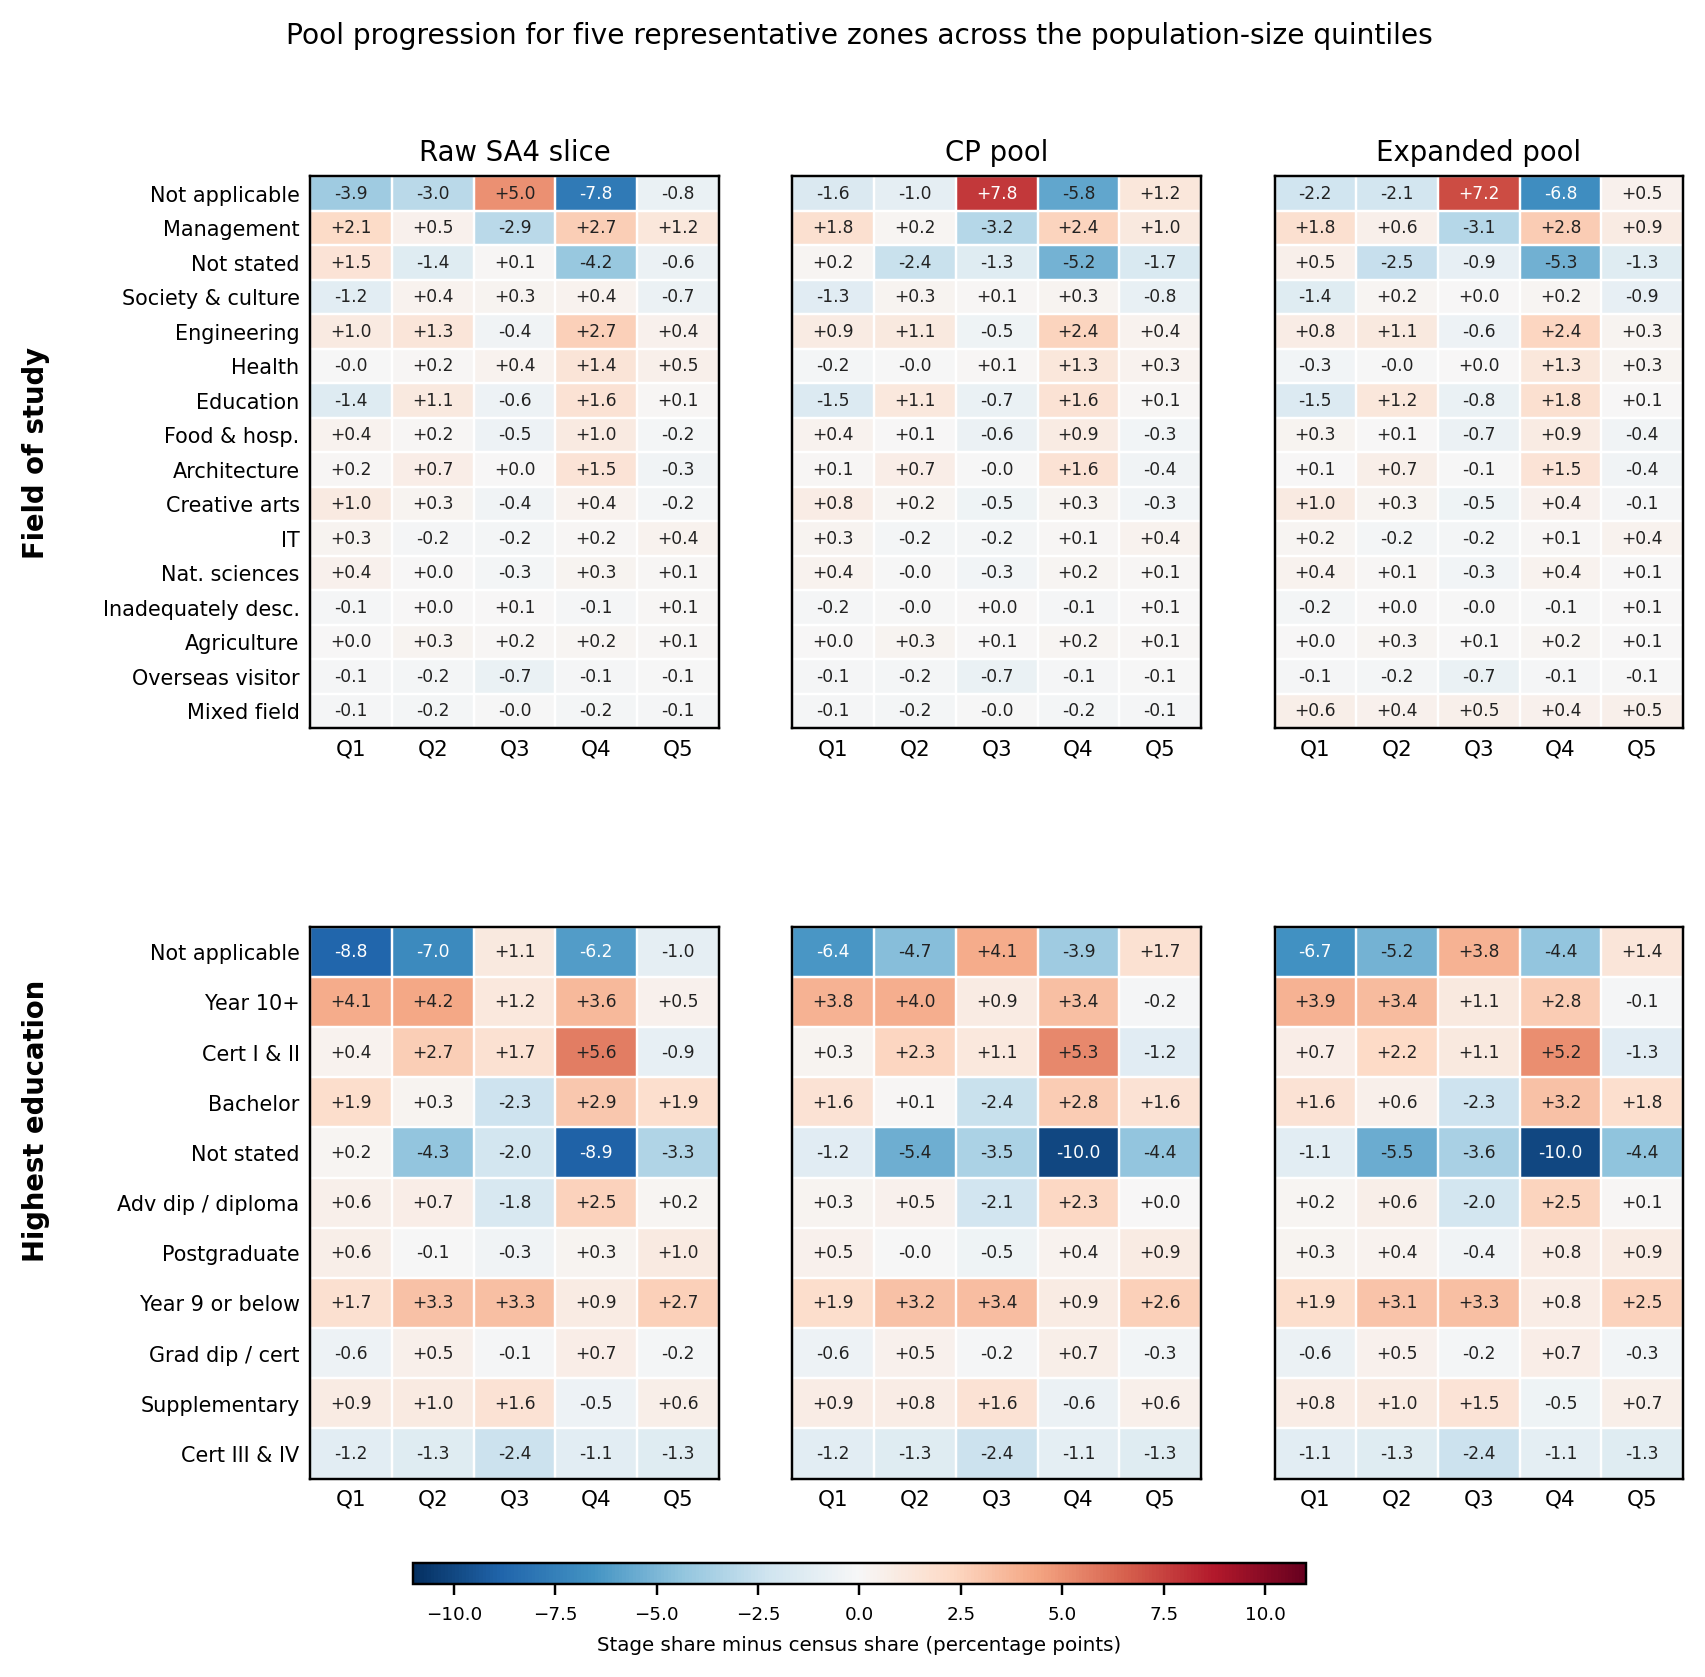
\includegraphics[width=\textwidth]{fig_pool_progression_by_size.png}
\caption{Pool progression for five representative zones spanning the
population-size quintiles (Q1 smallest to Q5 largest). Rows are categories;
columns are zones; the three panels are the raw SA4 slice, the CP pool and the
fitted population from the expanded pool. Each cell is the stage share minus the
census share in percentage points. Blue = close to the census share, red = a
large gap in either direction; the sign is printed in each cell (positive =
over-representation, negative = under-representation). The fitted panel is the
expanded population after carriers and zone fitting and shows the rebalancing
that the fitting stage provides.}
\label{fig:pool_progression_by_size}
\end{figure}

\input{files/expansion_added.tex}

\Cref{fig:zero_coverage_heatmap} shows the same coverage in terms of the
zero-capacity cells: it gives the cap-adjusted deficit coverage by control table
and zone population quintile. Most tables reach 100\% in every quintile;
relationship in household falls from 98.2\% in the smallest zones to 51.7\% in
the largest, and student status falls to 81.3\% in the largest.

\begin{figure}[H]
\centering
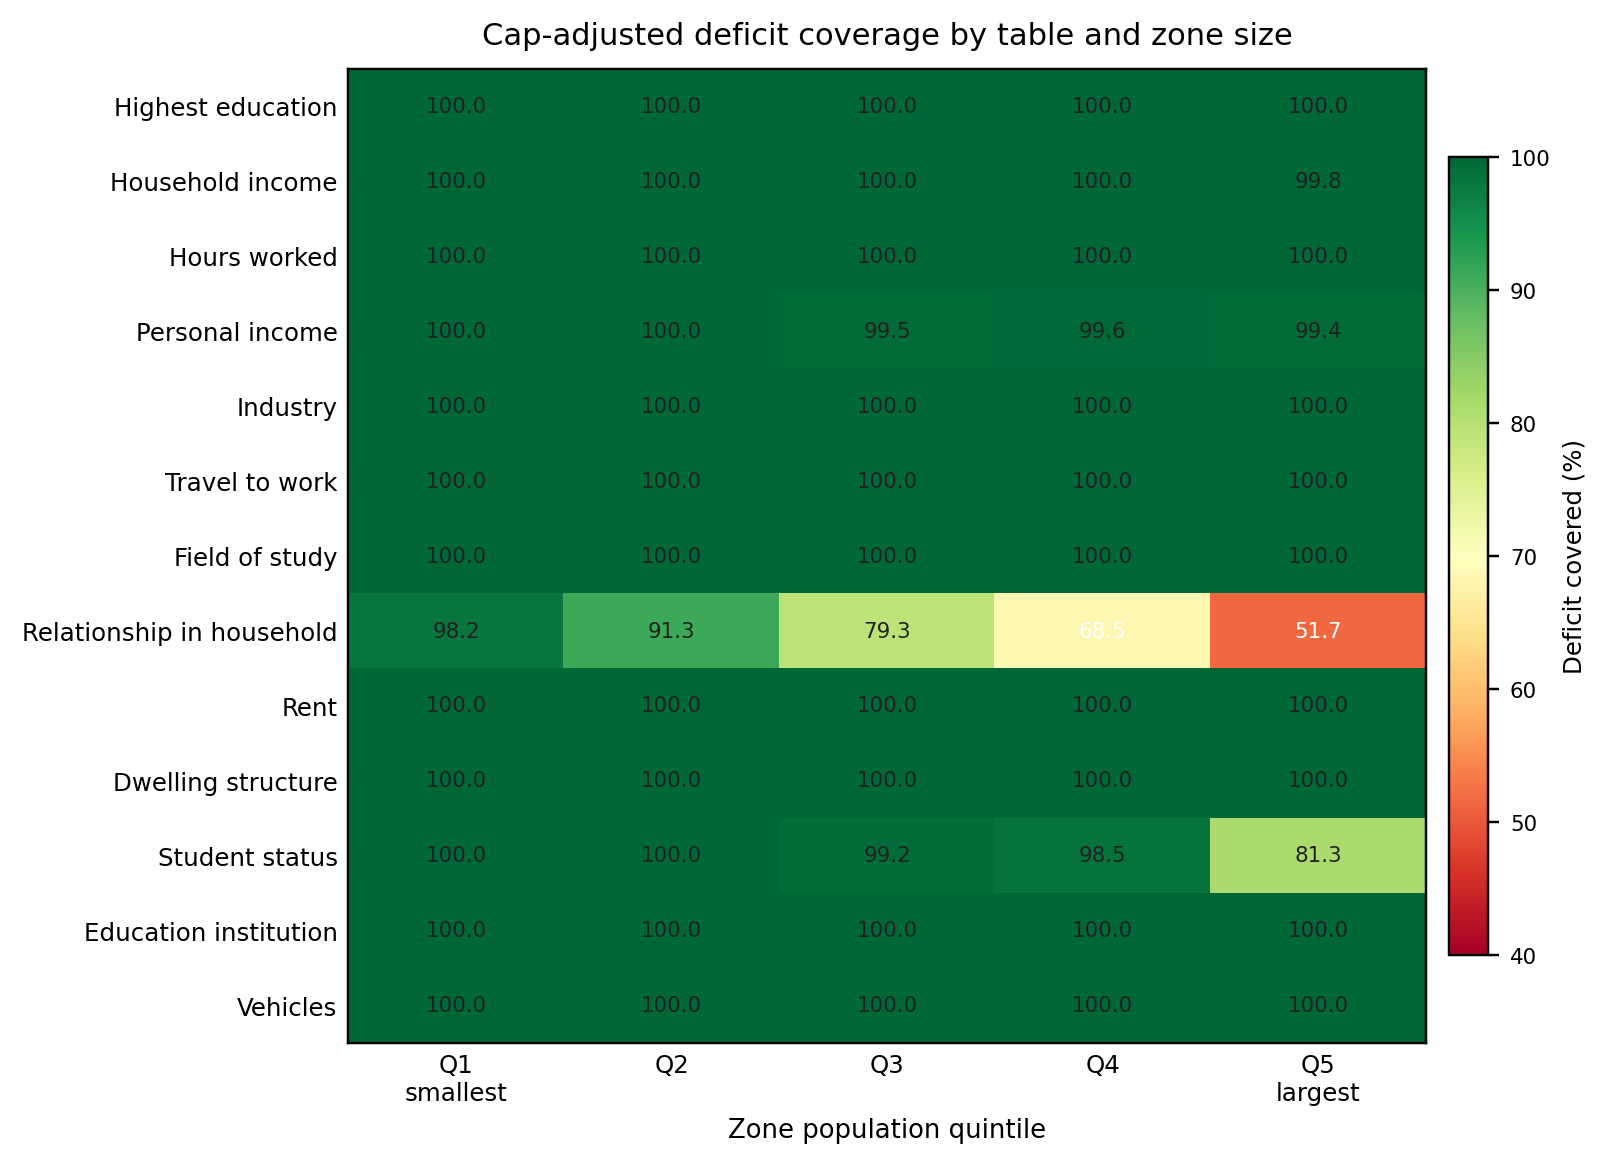
\includegraphics[width=0.86\textwidth]{fig_zero_coverage_heatmap.png}
\caption{Cap-adjusted deficit coverage of zero-capacity cells by control table
and zone population quintile. The value is the mean share of the cap-adjusted
deficit supplied by constructed carriers; 100\% means the deficit is reachable
at the replication cap. Lower values indicate cells where the carrier set is
short.}
\label{fig:zero_coverage_heatmap}
\end{figure}

\Cref{fig:zero_cell_status} turns the same audit into counts: each bar is the
number of zero-capacity cells in a table, green where the carrier set reaches
the deficit at the cap and red where it does not. The number in parentheses is
the count of cells with zero CP-pool capacity, i.e.\ no census donor.

\begin{figure}[H]
\centering
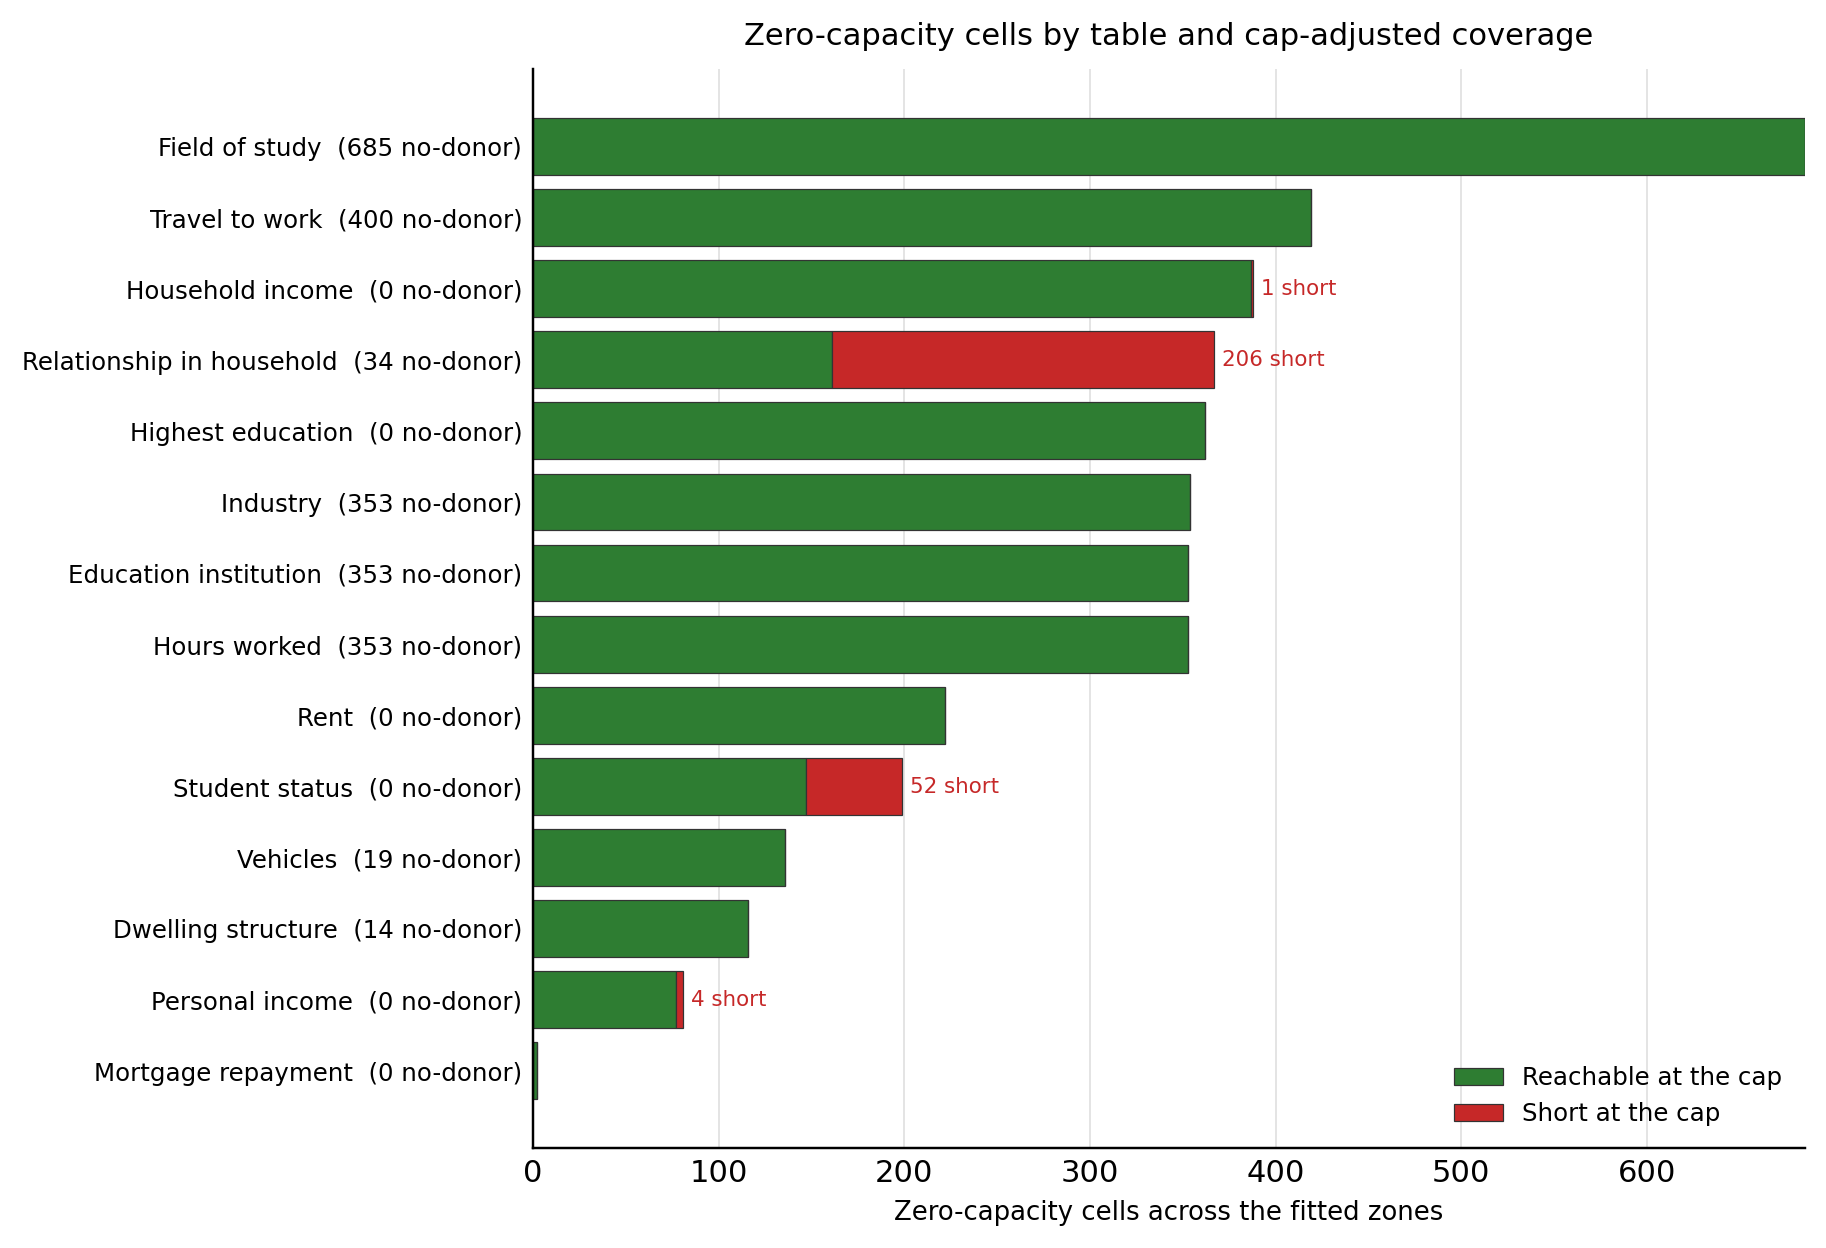
\includegraphics[width=0.9\textwidth]{fig_zero_cell_status.png}
\caption{Zero-capacity cells by control table and cap-adjusted coverage. Green
= the carrier set reaches the deficit at the replication cap; red = it does
not. The number in parentheses is the count of cells with zero CP-pool capacity
(no donor).}
\label{fig:zero_cell_status}
\end{figure}



\Cref{fig:pool_score_summary} reduces the pool stage to three summary scores:
the mean marginal distance, the share of zero-capacity cells with a carrier,
and an equal-weight composite of the two. Construction alone is marginally
neutral, expansion covers 13.3\% of the zero cells, and the constructed carriers
cover all
of them at no marginal cost. The composite is illustrative rather than a formal
utility; it makes the support--marginal trade-off visible in one place.

\begin{figure}[H]
\centering
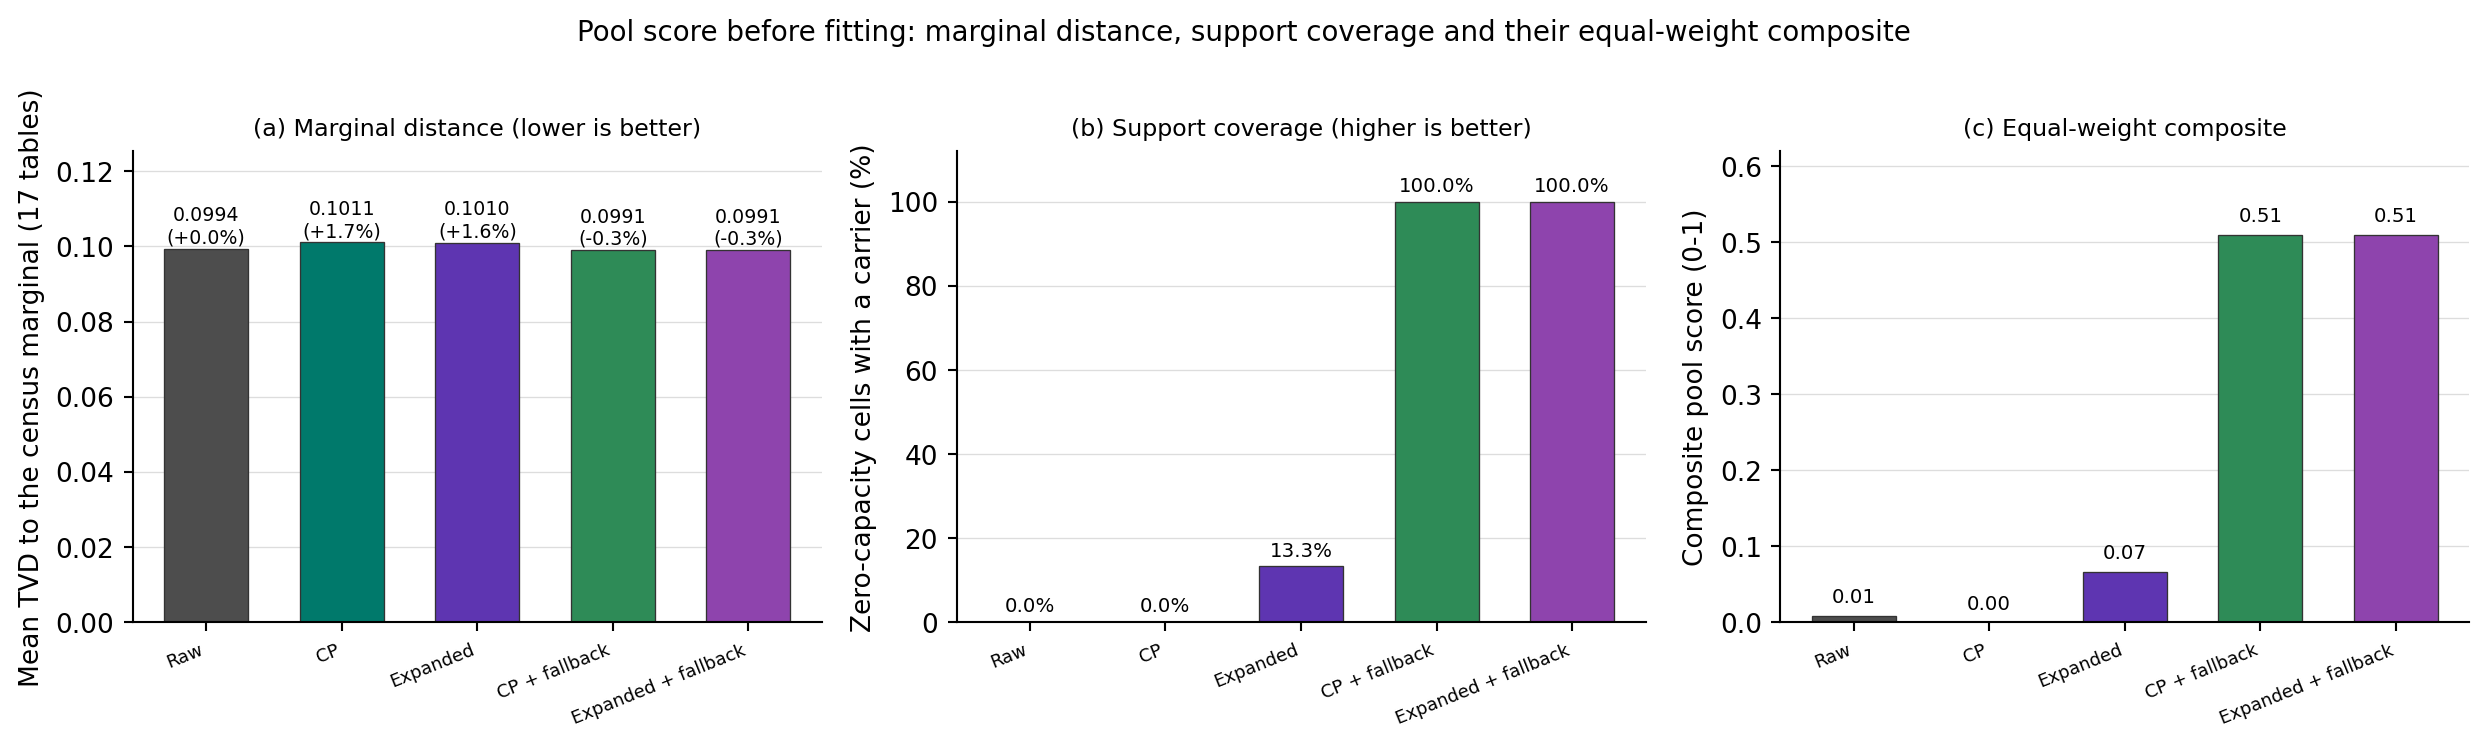
\includegraphics[width=\textwidth]{fig_pool_score_summary.png}
\caption{Pool score before fitting. (a) Mean TVD to the census marginal over
all 19 control tables. (b) Share of the 2{,}890 zero-capacity cells that have a
carrier. (c) Equal-weight composite of the normalized marginal score and
coverage.}
\label{fig:pool_score_summary}
\end{figure}

\subsection{Fit quality}
\label{sec:benchmark}

\cref{fig:rssz_by_arm} shows the full per-zone 19-table RSSZ distribution
for the base microdata, the two pools and four fitting methods.

The candidate set for each zone is thinned before the program is built.  The
donor block carries thousands of visitors-only or non-classifiable dwellings
(NPRD${}=7$), whereas the census marginal asks for only a trace number.  Left
uncapped, the integer program uses them as cheap carriers of visitor
relationship codes and the dwelling-size table absorbs the error.  The fit
therefore keeps at most $\max(20, 3\hat n_{\mathrm{NPRD}=7})$ such dwellings
per zone: enough to meet the target with replication and a margin, but not
enough to dominate the solution.

\input{files/fit_quality.tex}

\input{files/fit_repair.tex}

\begin{figure}[H]
\centering
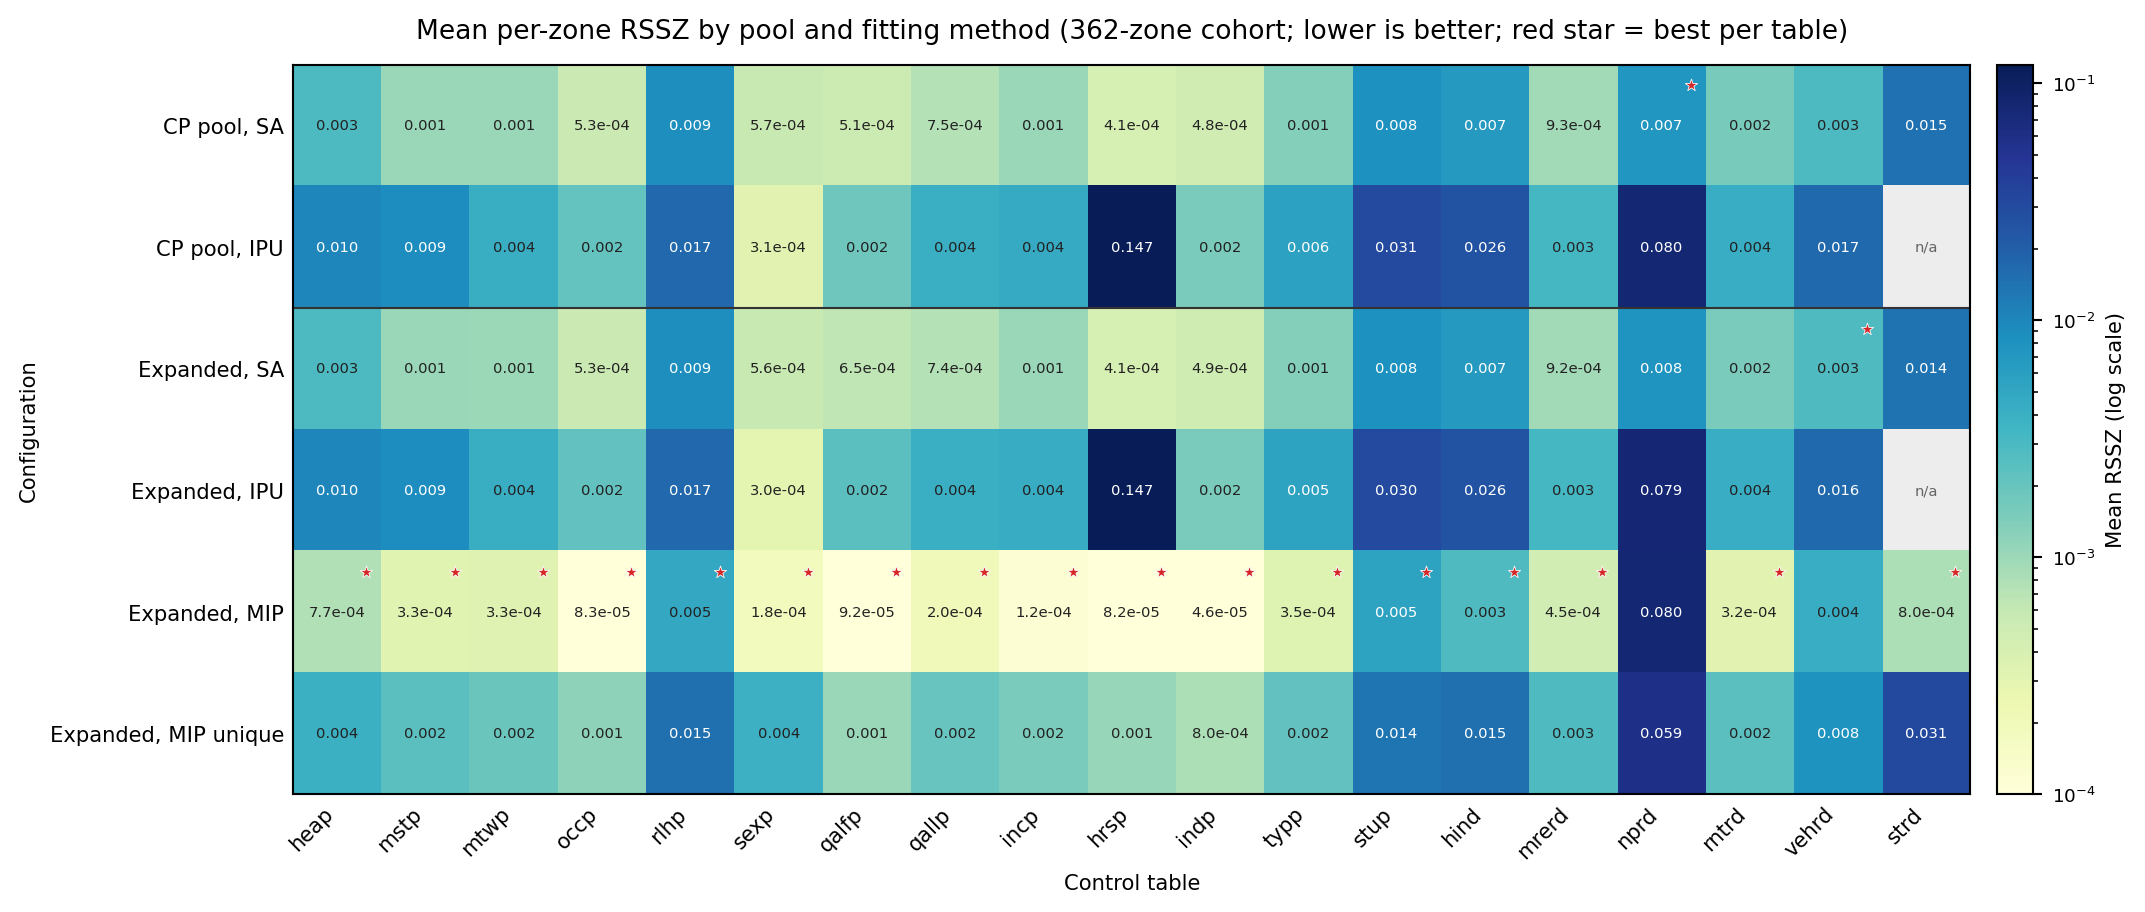
\includegraphics[width=\textwidth]{fig_method_table_heatmap.png}
\caption{Mean per-zone RSSZ by base microdata, configuration and control table
(log colour scale; lower is better). Rows are the base microdata fitted by SA
and IPU and the six configurations; columns are the 19 fitting tables. The red
star marks the lowest mean in each column. Base SA covers 325 of the 362
cohort zones and base IPU covers 362; the six fitted configurations cover 362.}
\label{fig:method_table_heatmap}
\end{figure}

\begin{figure}[H]
\centering
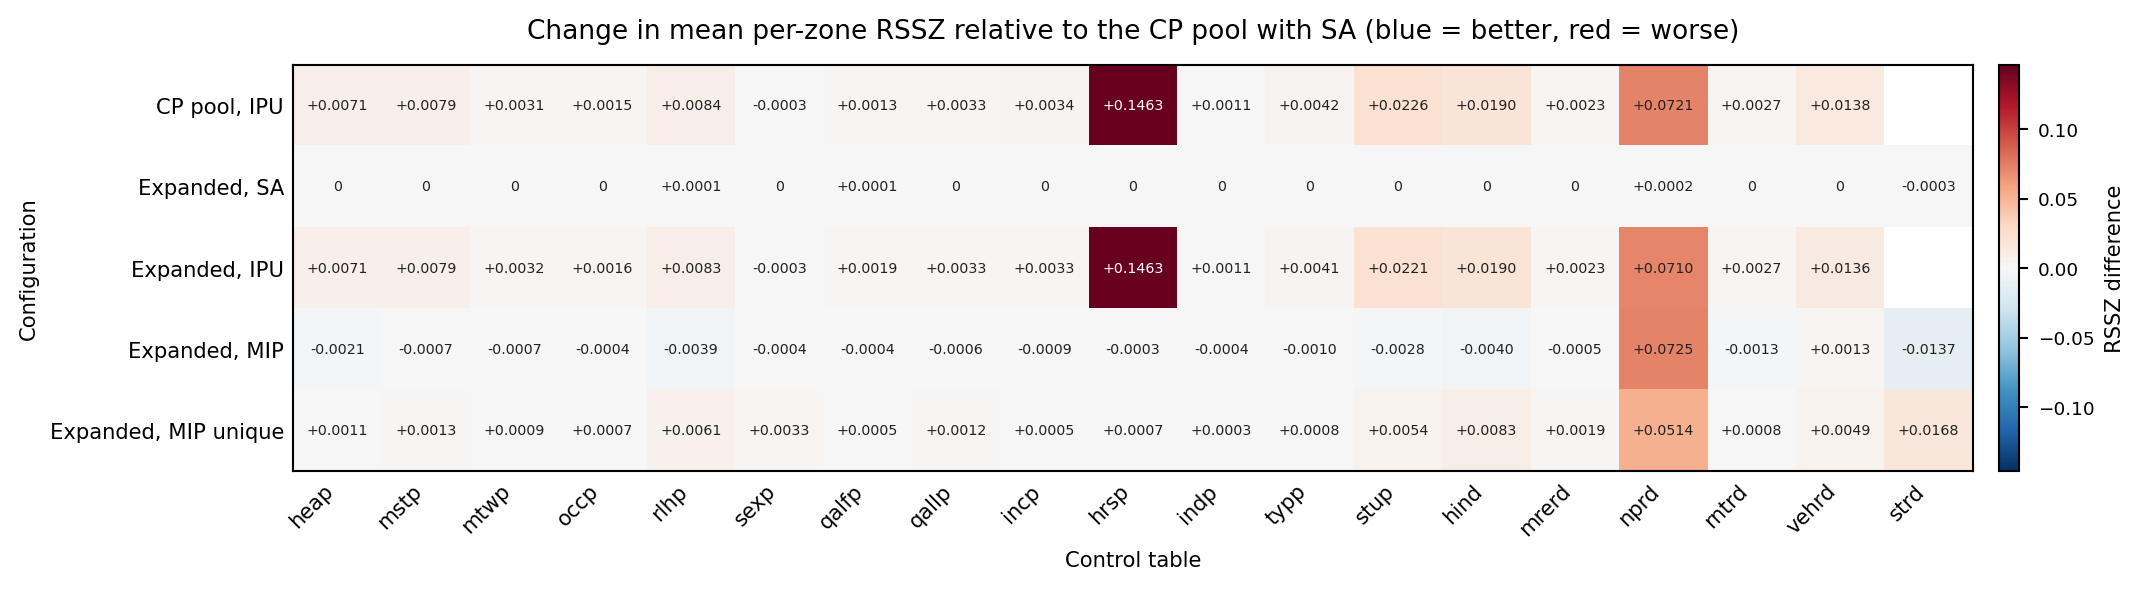
\includegraphics[width=\textwidth]{fig_table_delta_heatmap.png}
\caption{Change in mean per-zone RSSZ relative to the CP pool with SA for the
base microdata and the other five configurations (blue = better, red = worse).
The base rows show the raw microdata relative to the CP pool; the fitted rows
are the block ablations.}
\label{fig:table_delta_heatmap}
\end{figure}



\begin{figure}[H]
\centering
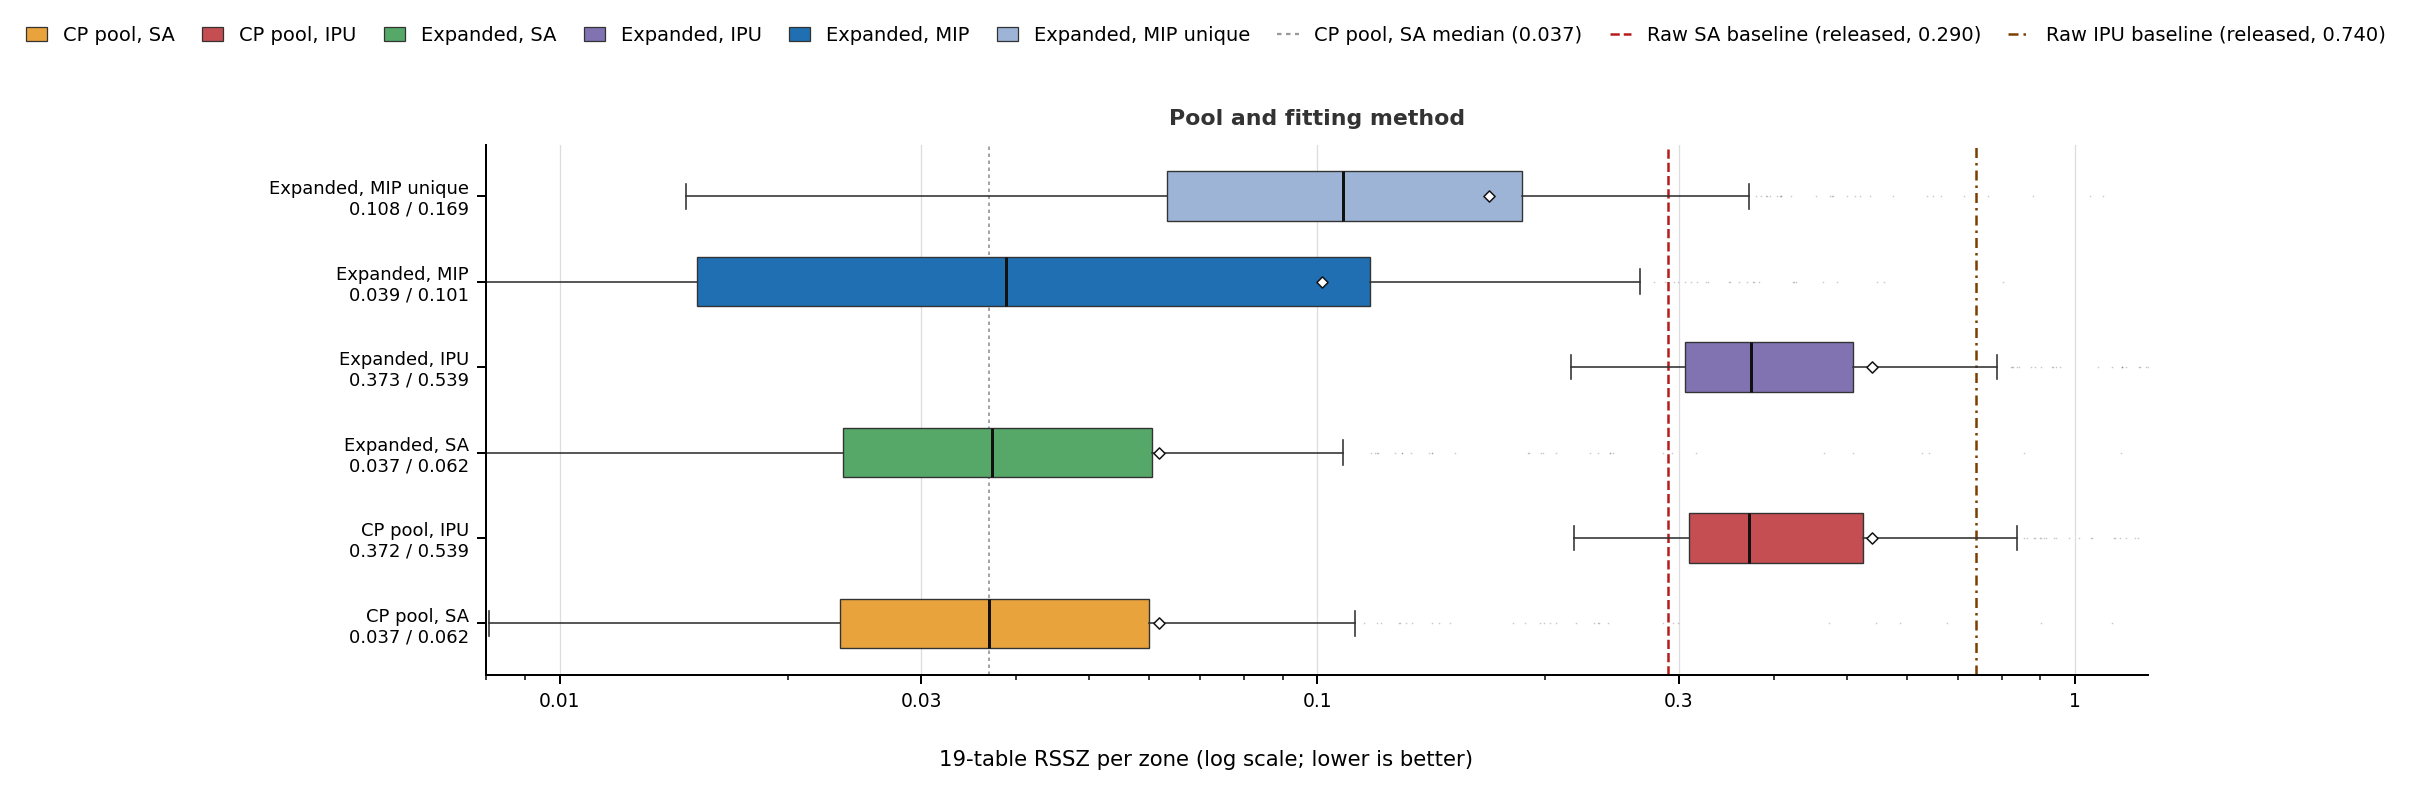
\includegraphics[width=\textwidth]{fig_rssz_by_arm.png}
\caption{Per-zone 19-table RSSZ across the 362 fitted zones for the base
microdata, the two pools and four fitting methods. Each row gives the
configuration and its median / mean RSSZ; the box shows the quartiles, the
black line the median, and the white diamond the mean. Base SA covers 325
zones and base IPU 362. The dotted line marks the CP pool with SA median
(0.037), the red dashed line the corrected-control raw-SA median (0.202,
325 zones), and the brown dash-dot line the corrected-control raw-IPU median
(0.525). Lower is better.}
\label{fig:rssz_by_arm}
\end{figure}







%\subsection{What the pool adds over the microdata}
%\label{sec:pool_delta}
%The comparison so far is between pools. \cref{tab:pool_delta} restates the
%same runs as a difference from the microdata, which is the state a zone
%synthesiser starts from: for each fitter the columns move from the raw extract,
%to the CP feasible pool, to the pool with the MIP expansion, so a metric family
%is read along a row rather than within one strategy. The pool changes three things
%and they do not move together.
%
%\textbf{Marginal fit.} Both fitters improve, on both bases. The 19-table median
%falls from 0.290 to 0.239 under SA and from 0.740 to 0.445 under IPU, and the
%11-table median from 0.233 to 0.163 and from 0.274 to 0.193. Part of that gain is
%household structure imposed at construction: the raw strategies select and reweight
%persons, so their household tables carry the drift documented in
%\cref{tab:hh_handling}, while a pool strategy selects whole households that were
%assembled under the eleven rules. Part of it is coverage, quantified below.
%Neither part requires a learned joint model, which is the point of the
%comparison.
%
%\textbf{Pooled shares say the opposite, and both readings are reported.}
%\cref{fig:categories_by_arm} pools every zone and compares each category
%share with the census. There the pool barely moves the aggregate: mean TVD over
%the eleven tables is 0.087 for SA-Only against 0.088 for CP-only + SA, and 0.106
%against 0.118 for IPU, the pool being worse on the two household tables it is
%meant to help (\texttt{nprd} 0.151 to 0.187, \texttt{vehrd} 0.088 to 0.105). The
%improvement in \cref{tab:pool_delta} is therefore a per-zone gain rather
%than a cohort-share gain: the pool fixes the composition of each zone's
%population, and zone-level errors of opposite sign cancel when the zones are
%pooled. A method read only on pooled shares would score the pool as neutral; a
%method read only on per-zone RSSZ would score it as uniformly better. Neither
%reading is reported alone.

%\textbf{Joint structure and diversity.} The marginal gain is not matched by a
%joint gain, and the direction depends on the fitter. Against the raw microdata
%the expanded pool moves the mean joint TVD from 0.051 to 0.099 under SA and from
%0.136 to 0.121 under IPU, raises the identical-person share from 3.8\% to 14.0\%
%under SA and lowers it from 6.5\% to 2.7\% under IPU, and leaves cross-zone
%cloning at 100.0\% under SA while lowering it from 98.7\% to 56.6\% under IPU.
%The pool therefore buys marginals, not association: under SA it buys them with
%repeated whole households, and under IPU with a reweighted but smaller distinct
%tuple set. The CP-only pair is marked --- because the joint audit was run on the
%published build and not re-run for it, so the pool's joint effect is measured
%only through the expanded pool and is stated as such rather than inferred.

%\textbf{Coverage, and what it costs.} The pool's addition to the microdata is
%concrete and countable: over the 362 fitted zones the expansion step addresses
%2{,}885 zero-capacity cells, covers 2{,}502 of them at their carrier requirement
%(87\%), and leaves 383 that its own ledger names --- 350 \texttt{qalfp:16}, the
%overseas-visitor supplementary code the fused qualification column does not
%carry, plus 19 \texttt{vehrd:6} and 14 \texttt{strd:6} cells with no
%rule-feasible donor--shell construction. Paying for that coverage costs
%5{,}592 households and 19{,}958 persons appended to the pool, and it costs
%replication at fit time, which is the trade the one-MIP pair isolates: the
%rep-1 adult-unique variant gives up 0.146 of the 19-table mean (0.076 to 0.222)
%to remove within-zone repeats, so the replication column of








%%%\textbf{The one-MIP strategies.} CP-MIP replaces the selection/weighting fitter with one integer program per zone. It chooses an integer replication count for every candidate household in the zone's SA4 slice, minimising missed control cells first and table deviations second, with a pool-anchored soft block for joint and uncontrolled attributes. \cref{tab:pool_fitter_matrix} shows that on both bases it has the lowest mean and median of any strategy: the sweep-winner setting (REP\_MAX~4, $\lambda_{\mathrm{joint}}$~20) is reported. The two zones that dominated earlier drafts no longer carve the mean: 302031036 is excluded with the non-residential group (\cref{tab:pathological_zones}), and 316071546's \texttt{nprd} collision no longer dominates its fit (0.078 in the refit); the largest remaining zone is 313021367 at 2.05, and excluding it moves the fitting mean only from 0.076 to 0.070, so the median is reported beside the mean and the mean is not read as the
%%%typical zone. Uniqueness costs fit: the rep-1 adult-unique variant raises the 19-table median from 0.053 to 0.156 and the mean to 0.222 while keeping every adult tuple distinct inside its zone, so replication is quantifiably what buys the marginal fit. \cref{tab:full_audit} shows the audit-level cost on the earlier build, with the highest within-zone duplication and joint TVD of its cohort; the re-audit of the refit and unique populations is a released script and is listed as pending. The released sweep summary reports the grid, where the identical-person share falls monotonically as the replication cap is lowered. The duplicate-penalty formulation is implemented in the released solver ($\lambda_{\mathrm{dup}}$, with a penalty term duplicating each selected tuple beyond its first use) and penalising duplicate tuples directly in the objective on the fitting basis remains future work.

%The construction and expansion stages do not reproduce zone totals: the pool is
%built once over the whole census, and the expansion step only restores cells
%that a zone's slice cannot supply, using the zone's marginal shares only to
%choose among coverage-equivalent sets. Zone totals enter at fitting, and in the
%one-MIP strategy they enter as explicit constraints over every candidate household,
%with missed cells counted and penalised ahead of deviation. The division is
%deliberate: putting 362 different zone targets into a pool built once would make
%the pool zone-specific and duplicate the fitter. Where the pool cannot source a
%cell, the miss count in the released CP-MIP summary records it, and those
%misses concentrate in the zones with the thinnest dwelling coverage.

%\cref{tab:pathological_zones} isolates the zones that stressed the constructed-pool fitters. In 302031036 the pool lacks the dwelling records needed for \texttt{rntrd}, \texttt{mrerd} and \texttt{vehrd}, and its person tables disagree on the universe (seven total 125--128, six total 837--851); it is a genuine data defect and is excluded with the five non-residential zones (\cref{tab:cohorts}). In 112011237 the earlier failure was the household-size trade-off from the non-private donors, which the corrected pool removes --- its MIP+SA drops from 3.64 to 0.15 --- so on the corrected pool only MIP+IPU stays mildly elevated (1.55); it stays in the cohort means. Neither is evidence about the fitter.
%
%\begin{table}[h!]
\centering
\caption{Zones where both fitters fail on the current MIP-expanded pool.
Entries are 11-table RSSZ on the 367-zone basis; SA-Only is shown for
reference. 302031036 also has internally inconsistent person-table totals (in
the 19-table fitting set, seven total 125--128 and six total 837--851); both
zones are treated as data or pool defects, not as fitter failures.}
\label{tab:pathological_zones}
\footnotesize
\begin{tabular}{@{}lrrr@{}}
\toprule
Zone & MIP+SA & MIP+IPU & SA-Only \\
\midrule
302031036 & 13.45 & 27.57 & 0.016 \\
112011237 & 3.64 & 1.65 & 0.237 \\
\bottomrule
\end{tabular}
\end{table}


%\cref{tab:cp_sa_tail} is the earlier diagnostic of the uncorrected-build MIP+SA tail, retained because it is how the problem was first localised: a longer seeded search improved four of the five worst zones, which already pointed to pool composition rather than search budget as the binding constraint. The corrected donor universe resolves all four of those directly --- on the corrected pool 112011237 falls from 3.64 to 0.15, 309071256 from 4.46 to 0.14, 314011386 from 3.67 to 0.24 and 303051073 from 2.92 to 0.78 on the 11-table basis --- confirming the tail was the non-private-dwelling donors, not the annealer. The fifth, 302031036, remains a data defect: its control tables disagree on the person universe (seven person tables total 125--128, six total 837--851), so no population can satisfy them and it is excluded from the fitted cohort.
%
%\begin{table}[h!]
\centering
\caption{Tail diagnostic on the five worst MIP+SA zones: the released
1{,}000-iteration run versus 5{,}000 iterations seeded from the MIP+IPU
allocation. Entries are 11-table RSSZ on the 367-zone basis. The MIP+IPU
value is shown for reference. Zone 302031036 is retained in the fixed cohort,
but its control tables disagree on the person universe: in the 19-table
fitting set, seven person tables total 125--128 and six total 837--851, so no
population can satisfy them all. Its
seeded row measures that data defect, not an iteration-budget effect; the other
four rows are the budget test.}
\label{tab:cp_sa_tail}
\footnotesize
\begin{tabular}{@{}lrrr@{}}
\toprule
Zone & MIP+SA 1{,}000 & MIP+SA 5{,}000 + seed & MIP+IPU \\
\midrule
302031036 & 13.45 & 18.31 & 27.57 \\
112011237 & 3.64 & 1.62 & 1.65 \\
309071256 & 4.46 & 1.05 & 1.12 \\
314011386 & 3.67 & 1.06 & 0.63 \\
303051073 & 2.92 & 0.64 & 0.68 \\
\bottomrule
\end{tabular}
\end{table}


\cref{fig:zone_size}
shows the share of zones with 19-table RSSZ above 1 by size quintile. The SA
and MIP fits stay at or below 3\% in every class, so they do not concentrate
poor fits in large zones. The IPU fits are higher---about 9--11\% in Q1 and
Q5---which is the same fitting-method gap the fit table reports. The differences
among the SA and MIP fits are small enough that the typical zone, not the tail,
is the object of the fit table.

\begin{figure}[H]
\centering
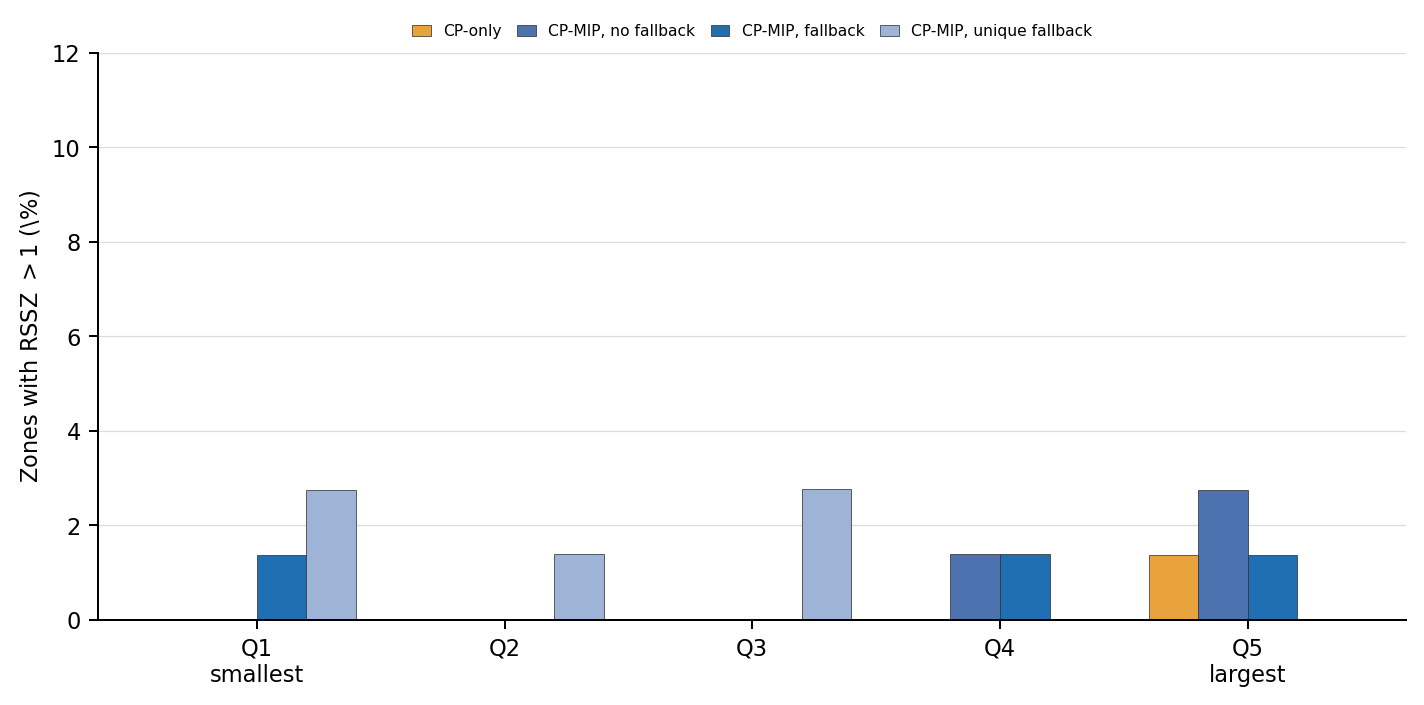
\includegraphics[width=0.78\textwidth]{fig_zone_size.png}
\caption{Share of poorly fitted zones (19-table RSSZ above 1) by census-population quintile, smallest (Q1) to largest (Q5). Lower is better.}
\label{fig:zone_size}
\end{figure}



\FloatBarrier

The worked example in \cref{fig:fit_example} shows one zone's per-table
residuals.

\begin{figure}[H]
\centering
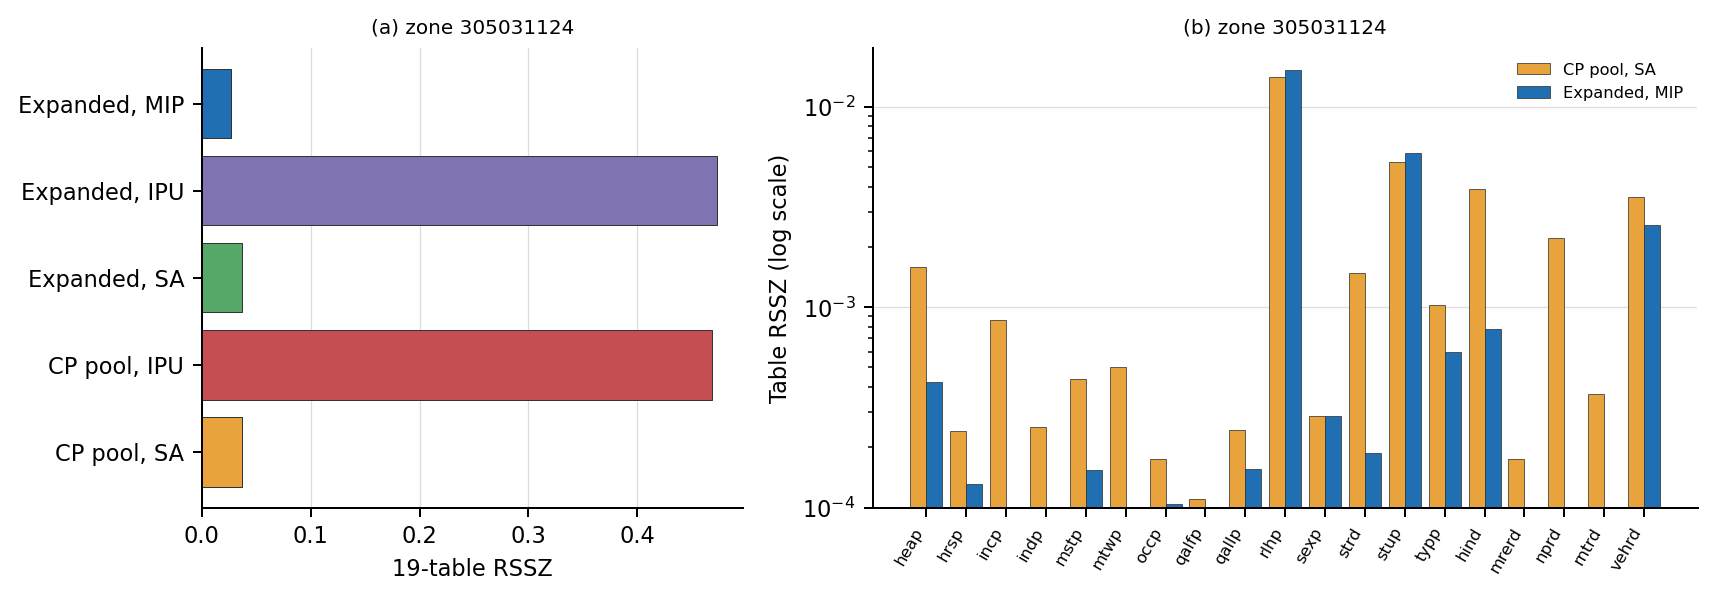
\includegraphics[width=\textwidth]{fig_fit_example.png}
\caption{Worked example for SA2 zone 305031124, at the CP pool with SA median.
(a) 19-table RSSZ by configuration, grouped by pool. (b) Per-table residuals
for the CP pool with SA and the expanded pool with MIP (log scale; values below
$10^{-4}$ at the axis floor).}
\label{fig:fit_example}
\end{figure}

\subsubsection{Held-out fit quality}
\label{sec:appendix_available_validation}
The fit optimises nineteen control tables. A further seven control tables are
held out of the fit entirely and never optimised. This section reports that
held-out validation: \cref{tab:heldout_rssz} for the base microdata, the two
pools and four fitting methods, and \cref{fig:heldout_tvd} for the paired-TVD
distances.
\Cref{tab:heldout_rssz} uses the RSSZ normalisation of the fitting objective;
\cref{fig:heldout_tvd} uses the total-variation share distance, so the two are
not comparable in level.

The held-out tables are never optimised, so they show what each configuration
carries into a margin it was not asked to match. The base microdata means are
0.101 (SA) and 0.139 (IPU). The expanded pool with SA gives the lowest held-out
mean (0.099), the CP pool with SA is 0.104, and the expanded pool with MIP is
0.190. The MIP fit is therefore the best on pooled marginal distance but not on
held-out error; the SA fit generalises better, and construction does not
improve held-out accuracy over the raw microdata.  With the structural
relationship repair and the visitors-only cap, held-out error falls further:
0.0436 for the CP pool and 0.0420 for the donor-balanced pool
(\cref{tab:fit_repair}), below every six-configuration row of
\cref{tab:fit_quality}.  The repair therefore improves held-out accuracy as
well as marginal fit.



\begin{table}[h!]
\centering
\caption{Held-out RSSZ by table for the completed arms on the 367-zone fitted
cohort. Entries are mean per-zone RSSZ with the median in parentheses; lower is
better. Each cell uses the zones where that table is defined for both the arm
and the census. The seven tables were excluded from the fitting basis.
\texttt{lfsp} is scored on 258 zones for RSSZ; \texttt{hcfmf} needs
\texttt{families\_in\_household}, which the two raw arms do not carry.}
\label{tab:heldout_rssz}
\footnotesize
\setlength{\tabcolsep}{3pt}
\resizebox{\textwidth}{!}{%
\begin{tabular}{@{}lrrrrrrr@{}}
\toprule
Held-out table & SA-Only & IPU-Only & CP-SA & CP-IPU & Comp-SA & Comp-IPU & CP-MIP \\
\midrule
age5p (age by 5-year group) & 0.012 (0.002) & 0.016 (0.003) & 0.008 (0.002) & 0.009 (0.003) & 0.007 (0.002) & 0.010 (0.004) & 0.007 (0.002) \\
assnp (need for assistance) & 0.186 (0.002) & 0.257 (0.002) & 0.194 (0.001) & 0.221 (0.001) & 0.262 (0.013) & 0.273 (0.011) & 0.050 (0.001) \\
bedrd (bedrooms)            & 0.174 (0.023) & 0.042 (0.018) & 0.057 (0.021) & 0.037 (0.017) & 0.059 (0.021) & 0.037 (0.018) & 0.032 (0.015) \\
hcfmf (family composition)  & n/a & n/a & 0.045 (0.043) & 0.067 (0.064) & 0.698 (0.386) & 0.579 (0.311) & 0.062 (0.057) \\
hhcd (household composition)& 0.095 (0.012) & 0.023 (0.014) & 0.018 (0.011) & 0.018 (0.013) & 0.019 (0.012) & 0.022 (0.017) & 0.020 (0.011) \\
lfsp (labour force status)  & 0.177 (0.037) & 0.263 (0.042) & 0.247 (0.038) & 0.256 (0.041) & 0.271 (0.042) & 0.280 (0.044) & 0.079 (0.038) \\
tenlld (landlord type)      & 1.097 (0.021) & 0.198 (0.015) & 0.203 (0.018) & 0.222 (0.013) & 0.125 (0.012) & 0.100 (0.011) & 0.959 (0.012) \\
\bottomrule
\end{tabular}%
}

\par\smallskip
{\footnotesize\textit{Note:} the RSSZ and TVD held-out tables differ by one
\texttt{lfsp} zone (258 here, 259 in Table~\ref{tab:heldout}) because RSSZ
requires a positive expected count in every cell. Several means are
heavy-tailed. Zone 302031036 is a non-private-dwelling SA2 whose household
controls carry at most 35 households, while every arm emits several hundred
households there, and whose person tables disagree on the universe (in the
19-table fitting set, seven total 125--128 and six total 837--851). It alone
accounts for most of the SA-Only means on
\texttt{assnp}, \texttt{hhcd}, \texttt{lfsp}, \texttt{tenlld} and
\texttt{age5p}, and for a large part of the \texttt{tenlld} mean of every arm.
The median in parentheses is the robust comparison; the mean is retained for
comparability with the main tables.
}
\end{table}


The held-out aggregate is dominated by landlord type. For the MIP fit its mean
RSSZ is 0.969, against 0.017 for the CP pool with SA and 0.017 for the expanded
pool with SA; the other six tables are closer. The held-out comparison therefore
separates the fit metrics: MIP buys pooled marginal fidelity, SA buys held-out
robustness.

\begin{figure}[H]
\centering
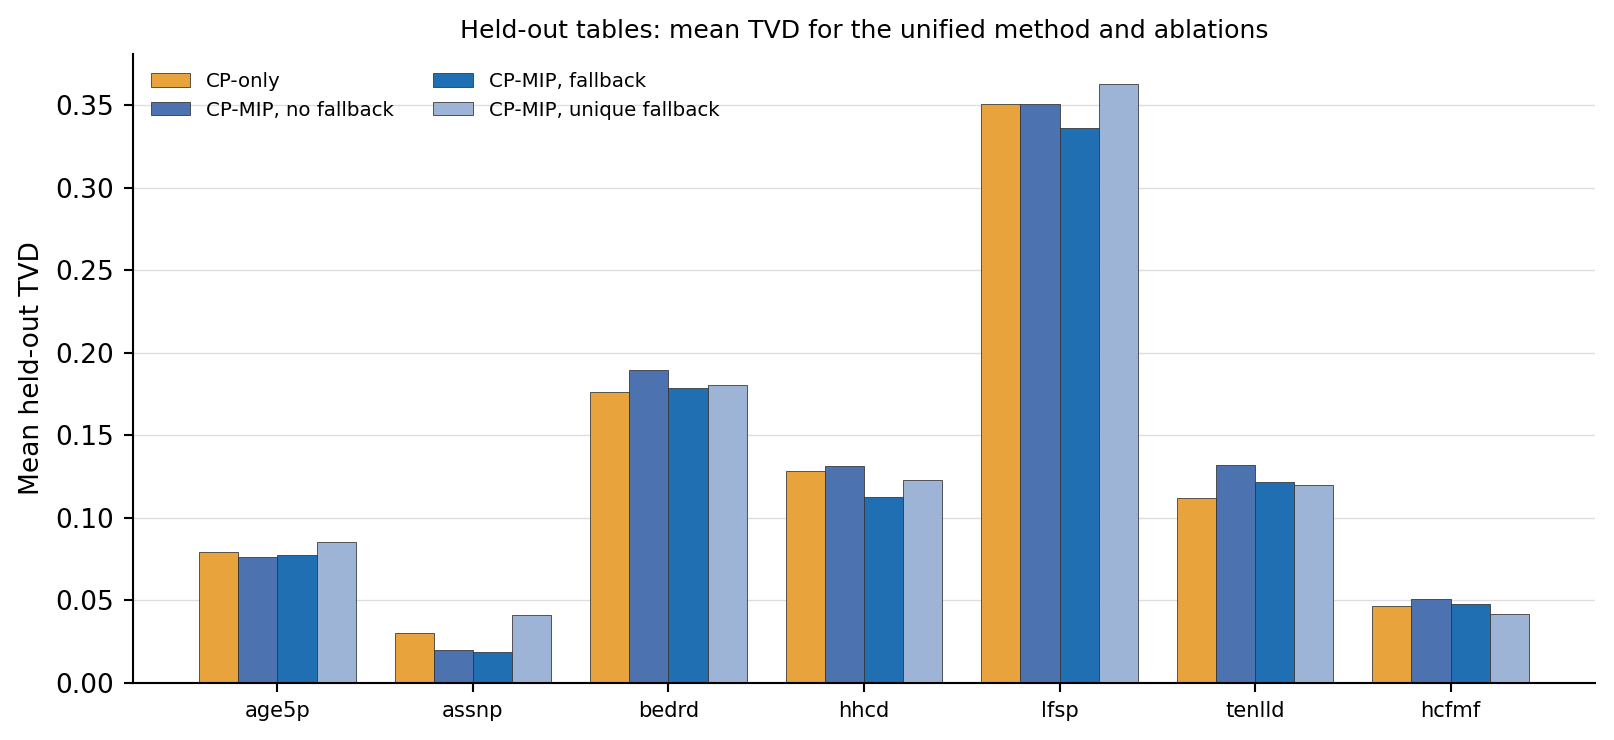
\includegraphics[width=\textwidth]{fig_heldout_tvd.png}
\caption{Mean held-out TVD for the seven held-out control tables across the six
fitted configurations. The base microdata held-out RSSZ is reported in
\cref{tab:heldout_rssz}; the TVD figure uses the paired-share distance and is
not computed for the base arms.}
\label{fig:heldout_tvd}
\end{figure}



\FloatBarrier



\clearpage
\subsubsection{Household travel survey attributes}
\label{sec:hhts_validation}
The 19 census control tables do not include the household travel survey
variables used by the ABM. The fused microdata carries observed Queensland
Travel Survey values for household bicycles, e-bikes and e-scooters and for
person car and motorcycle licences. Household variables are attached by
predictive-mean matching; person licences are attached by hot-deck within
five-year age band and sex using the person identifier. The CP/MIP pool
carries the attached columns, and the fit selects whole households and
persons, so the fitted population inherits them. The released population
applies this person-level attachment; the census-control fit tables are
unaffected because licences are not control variables.

\Cref{tab:hhts_validation} compares the fitted population with the attached
pool. The household bicycle distribution is close (no bicycle 53.5\% against
52.7\%, three or more 18.3\% against 20.4\%), and the fitted population
reproduces bicycle ownership by household size
(\cref{fig:hhts_validation}b). Car and motorcycle licence shares are 89.0\%
and 6.6\% among persons aged 15 and over, against 88.3\% and 6.6\% in the
attached pool and 88.2\% and 6.5\% in the survey. The age profile is also
reproduced (\cref{fig:hhts_validation}c): car licence rises from 67.2\% at
15--24 to 96.3\% at 35--44 and 85.4\% at 65 and over, against 65.6\%,
96.3\% and 83.9\% in the pool. The composition and cross-age matrices
(\cref{fig:hhts_validation}a,d) locate the remaining differences: one-family
and lone-person households are within about half a point of the pool, while
visitors-only households differ by up to 9.7 points and the 45--64
reference-person/45--64-member cell by 3.6 points. The cross-age matrix counts
each household member once against the household's reference person, so its
diagonal is the same-age block.

\begin{table}[H]
\centering
\caption{Household travel survey attributes in the fitted population and in
the attached pool. Car and motorcycle licences are computed over persons aged
15 and over.}
\label{tab:hhts_validation}
\begin{tabular}{lccc}
\toprule
Attribute & Fitted (\%) & Attached pool (\%) & Difference (pp) \\
\midrule
Bicycles: none            & 53.5 & 52.7 & $+0.8$ \\
Bicycles: one             & 11.8 & 11.2 & $+0.6$ \\
Bicycles: two             & 16.4 & 15.8 & $+0.7$ \\
Bicycles: three or more   & 18.3 & 20.4 & $-2.1$ \\
E-bike: one or more       &  1.8 &  2.4 & $-0.6$ \\
E-scooter: one or more    &  6.3 &  6.4 & $-0.1$ \\
Car licence (15+)         & 89.0 & 88.3 & $+0.7$ \\
Motorcycle licence (15+)  &  6.6 &  6.6 & $0.0$ \\
\bottomrule
\end{tabular}
\end{table}

The remaining gaps are e-bike ownership, households with three or more
bicycles, and some spatial variation (\cref{fig:hhts_spatial}). Apart from
the three-or-more-bicycle cells in Brisbane West ($+2.9$ points) and
Brisbane Inner City ($-4.0$ points), every SA4 cell is within $\pm2$
percentage points. Across zone-size quintiles, the three-or-more-bicycle
shortfall reaches $-2.4$ points in the fourth quintile and $-2.1$ points in
the largest, while licence differences remain within 1.2 percentage points.

\Cref{fig:hhts_validation} follows the carried attributes from the attached
pool, the pre-fit donor-attached state, to the fitted population, the expanded
state. Each cell therefore isolates what the fitting stage changes relative to
the raw donor-attached pool rather than mixing that change with the attachment
step itself.

\begin{figure}[H]
\centering
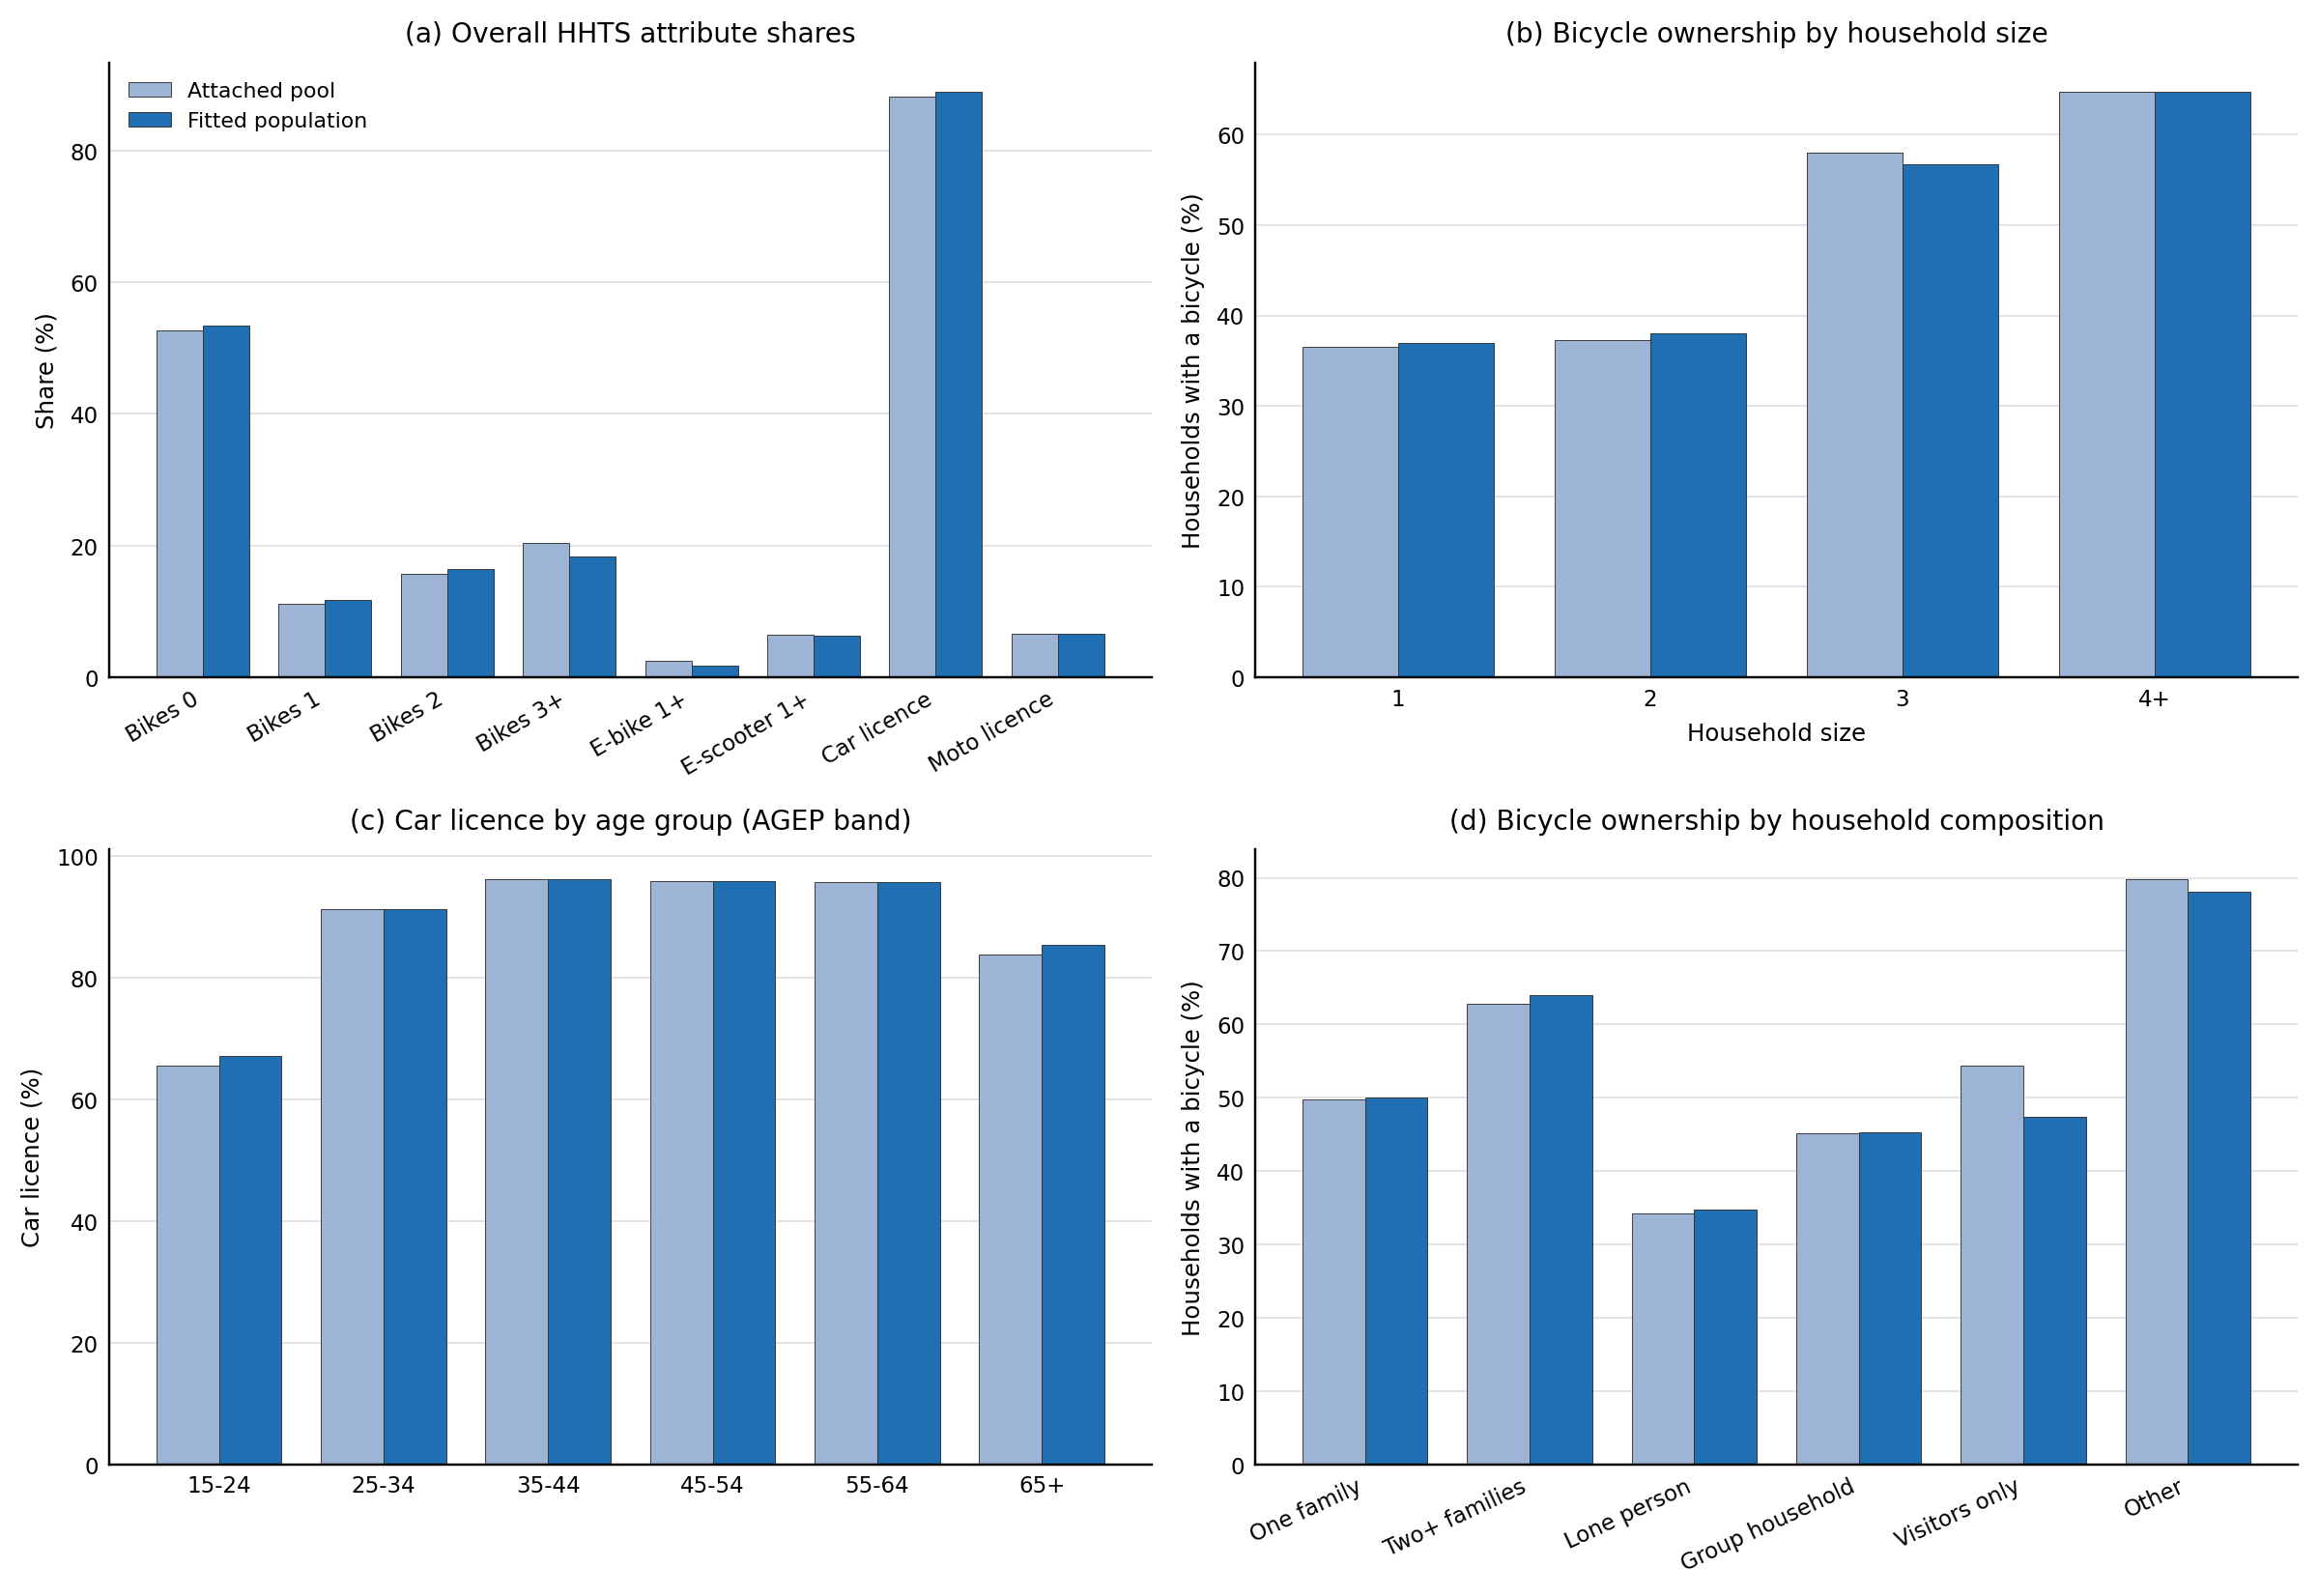
\includegraphics[width=\textwidth]{fig_hhts_validation.png}
\caption{Household travel survey attributes carried from the attached pre-fit
pool into the fitted, expanded population. (a) Household composition $\times$
bicycle count. (b) Household size $\times$ bicycle count. (c) Age band $\times$
licence. (d) Reference-person age $\times$ household-member age. Cells are
fitted minus attached-pool shares in percentage points: the attached pool is the
pre-fit state in which each census household already carries its HHTS donor
attributes, and the fitted population is the expanded state after zone fitting.
Blue = the fitted population under-represents the cell relative to the pre-fit
state, red = over-represents it. Each panel uses its own symmetric colour
scale.}
\label{fig:hhts_validation}
\end{figure}

\begin{figure}[H]
\centering
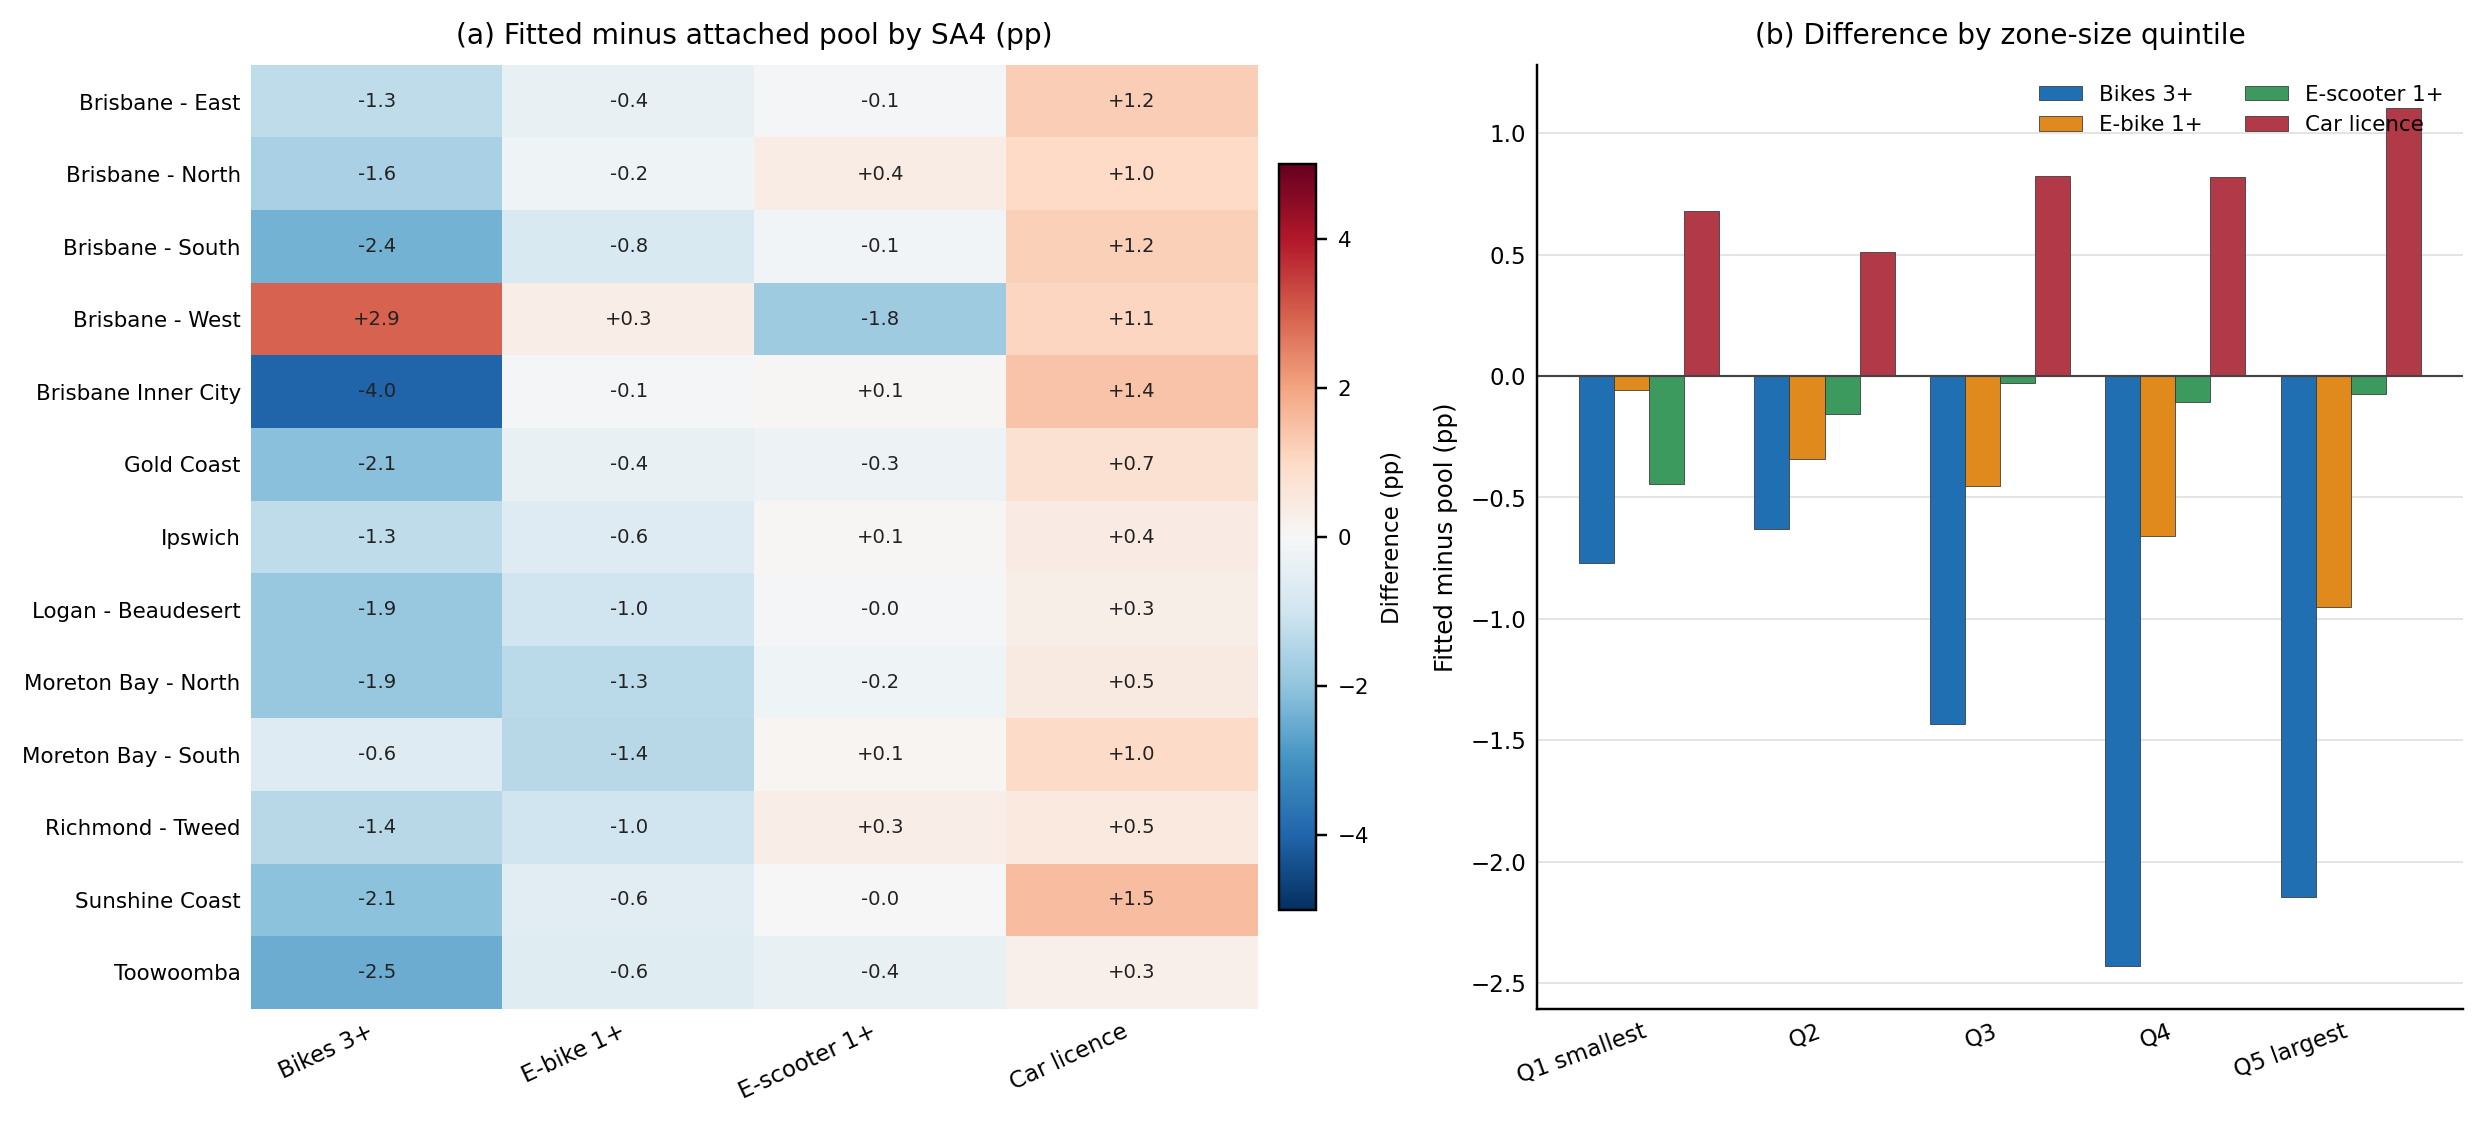
\includegraphics[width=\textwidth]{fig_hhts_spatial.png}
\caption{Household travel survey attributes by SA4 and zone-size quintile.
(a) Fitted minus attached-pool difference in percentage points by SA4.
(b) The same difference by zone-size quintile.}
\label{fig:hhts_spatial}
\end{figure}

Every one of the 362 zones draws on observed HHTS households
(\cref{fig:hhts_coverage}). The donor pool supplies between 4.8 and 13.2
observed households per 100 target households, so the fitted population
replicates observed donors rather than imputing household travel attributes.

\begin{figure}[H]
\centering
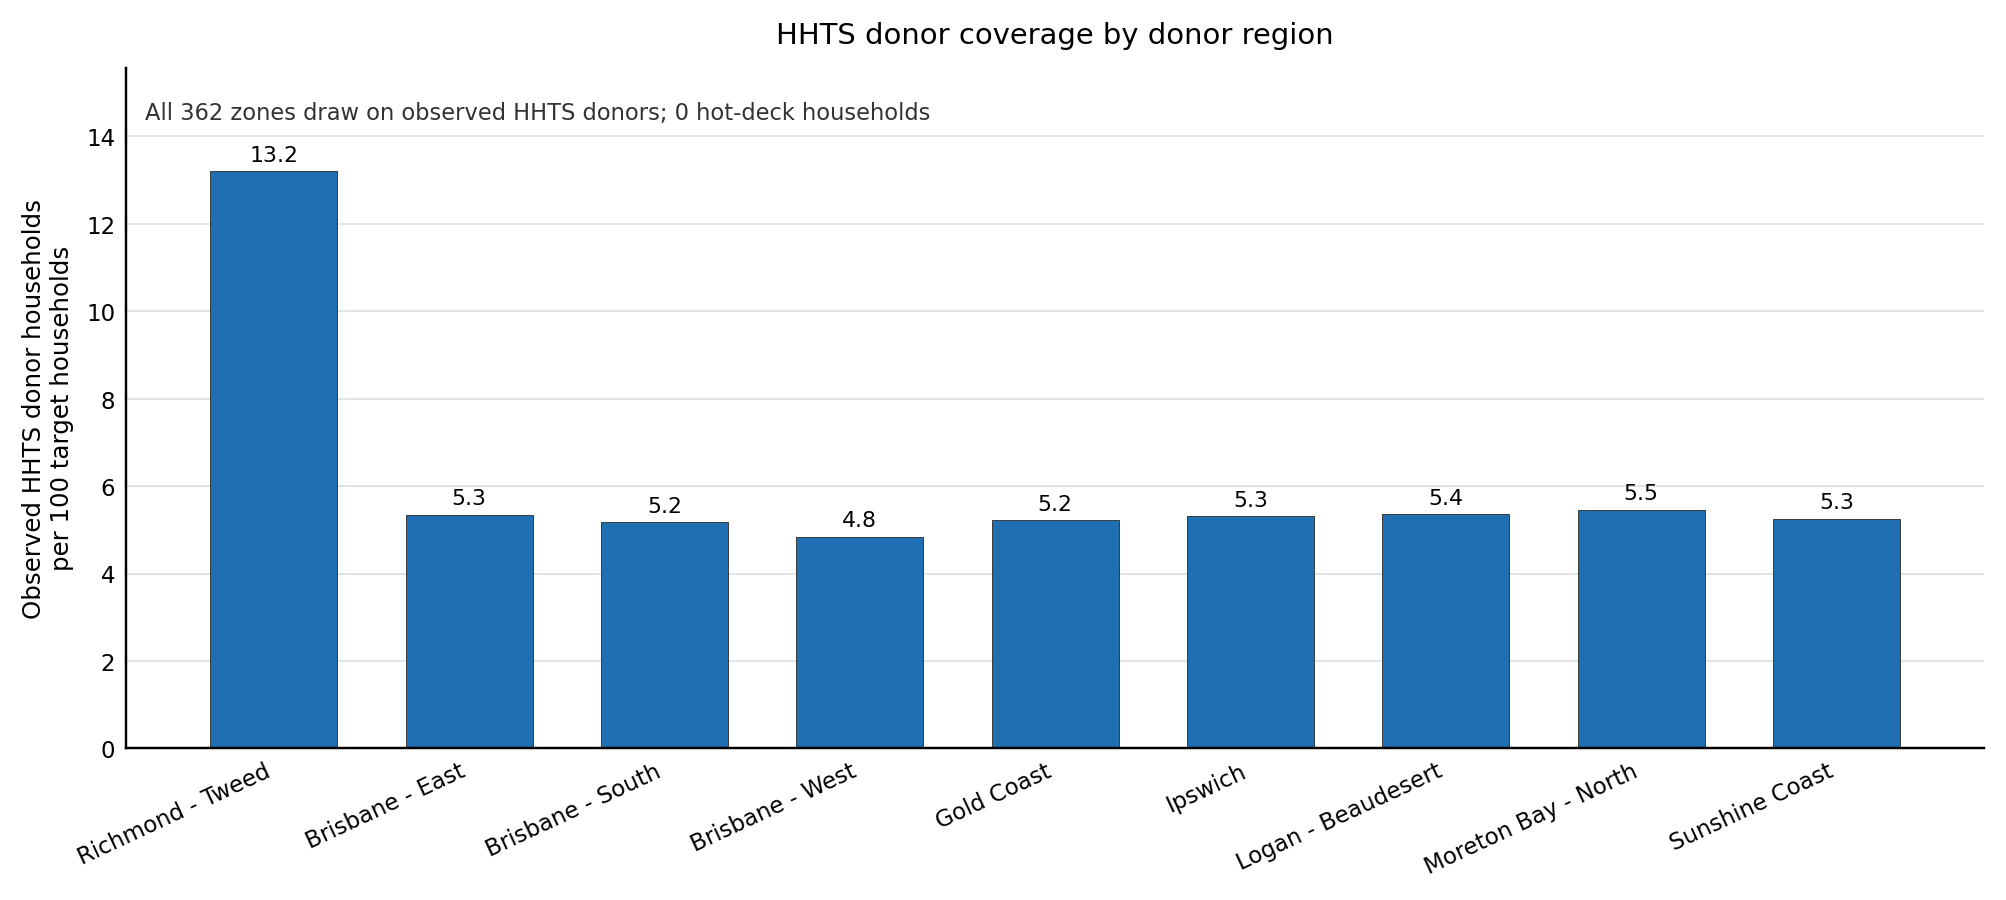
\includegraphics[width=0.92\textwidth]{fig_hhts_coverage.png}
\caption{Observed HHTS donor households per 100 target households by donor
region. All 362 zones have at least one observed donor household.}
\label{fig:hhts_coverage}
\end{figure}

The fitted population's spatial age structure follows the settlement pattern
(\cref{fig:age_spatial}). Children aged 0--14 and adults aged 25--44 are
concentrated in the outer suburban SA2s, people aged 15--24 in the inner city
and university catchments, and people aged 65 and over in the coastal and
rural SA4s. The total-population panel reproduces the settlement footprint of
the census controls. The SA2 boundary file used for the maps is released with
the paper.

\begin{figure}[H]
\centering
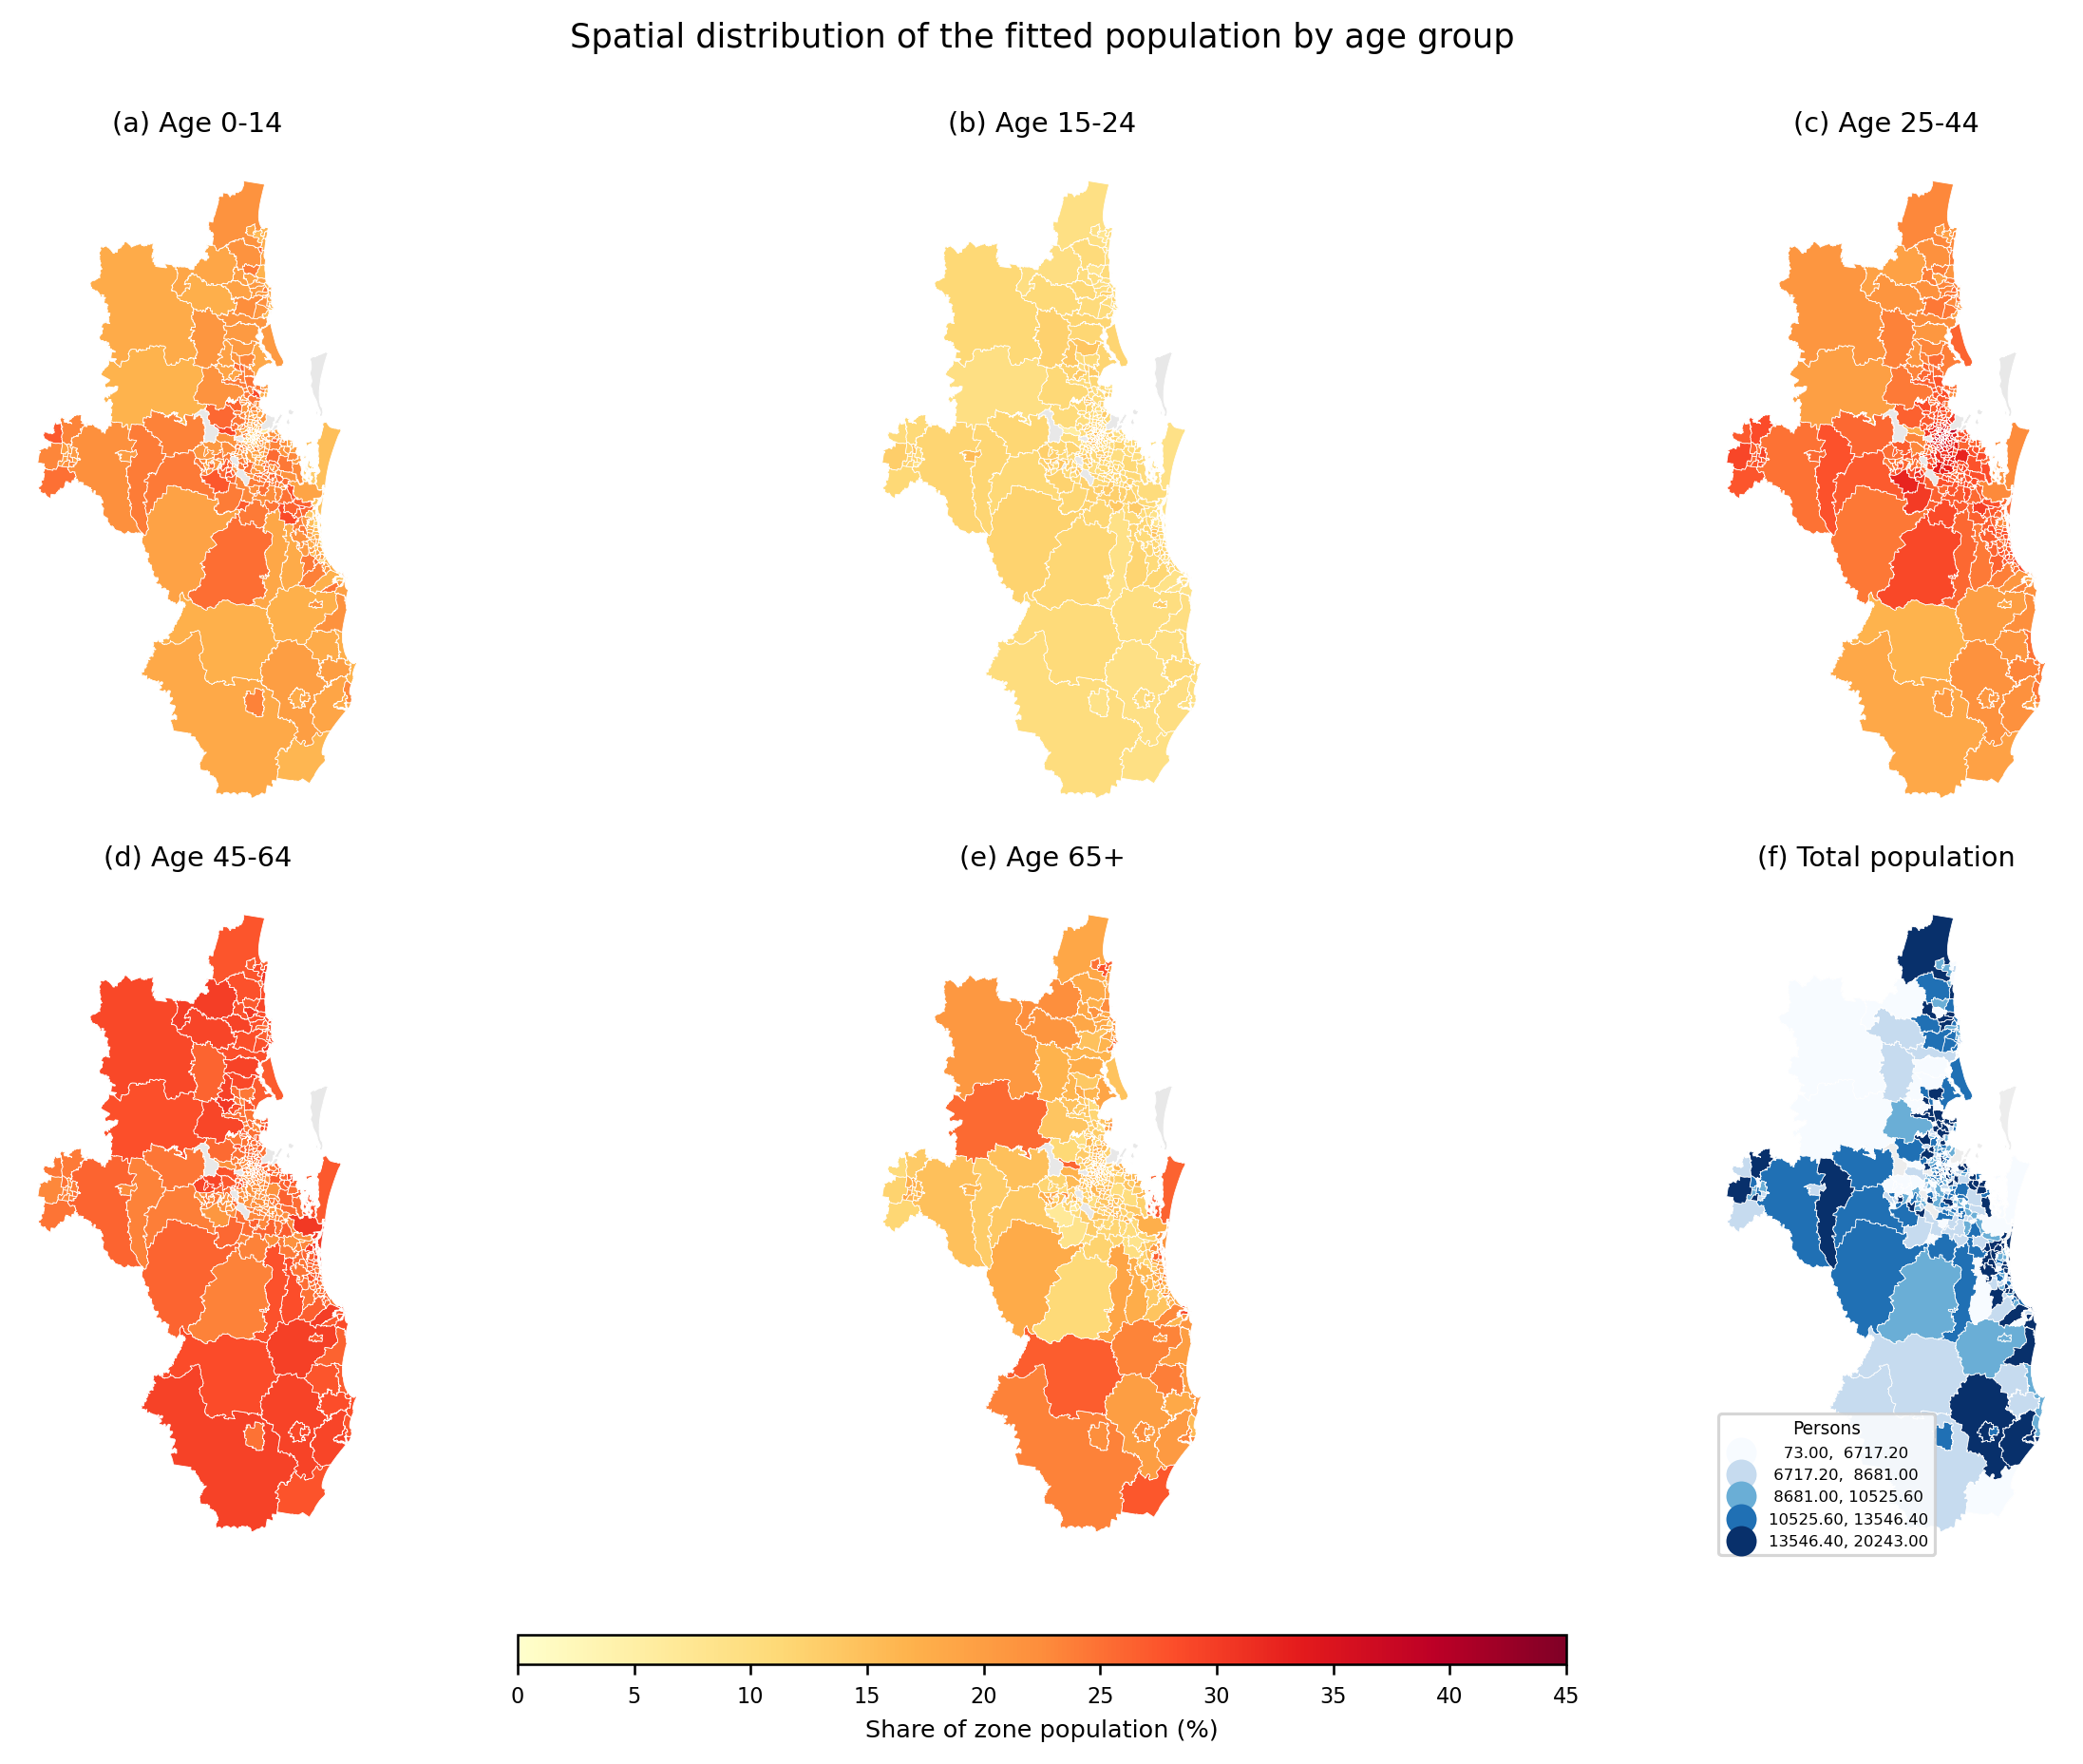
\includegraphics[width=0.92\textwidth]{fig_age_spatial.png}
\caption{Share of the fitted population in each age group across the 362 SA2s.
(a) 0--14, (b) 15--24, (c) 25--44, (d) 45--64, (e) 65 and over, and (f) total
population. Grey areas are SA2s outside the fitted cohort; boundaries are the
2021 ABS SA2s, released as \texttt{seq\_sa2\_2021.geojson}.}
\label{fig:age_spatial}
\end{figure}

The carried attributes are not part of the 19-table objective, so the fit has
no direct incentive to preserve their marginals. The fitting MIP therefore
accepts a soft block. For each attached attribute value $s$, a deviation
variable $g_s$ satisfies
\begin{equation}
g_s \;\ge\; \left|\sum_j B_{js} n_j - U_s\right|,
\end{equation}
where $B_{js}$ is the incidence of value $s$ in candidate household $j$,
weighted by the type's raw pool multiplicity, $U_s$ is the pool share times
the zone target, and the term enters the objective with weight
$\lambda_{\mathrm{joint}}/\max(U_s,1)$. Person licences enter through the
number of licensed persons in each candidate household. The block covers
bicycles, e-bikes, e-scooters, car and motorcycle licences, and the
household-composition-by-bicycle joint. The block is part of the released
fitting program; the fixed-edit tables in this paper use the
carried-attribute setting so that every configuration is compared on the same
19-table objective, and the soft block is reported separately because it
changes that objective.

\subsubsection{Downstream demand-model benchmark}
\label{sec:abm_validation}
The released population was passed through the stage 5/6 tour model and
compared with the weighted Queensland Travel Survey trip file
(\cref{tab:abm_validation}). The model produces 3.06 trips per person against
3.42 in the survey, and a mean trip length of 8.50 km against 7.75 km; the
trip-length distribution differs by 0.17 in total variation. The trip-rate
gap is model-side rather than population-side: applying the survey's segment
trip rates (3.53 for licensed and 3.14 for unlicensed persons) to the fitted
population's licence shares gives 3.42 trips per person, matching the survey
total. Mode shares are not yet reproduced: the stage model assigns 29.7\% of
trips to transit against 14.0\% in the survey, and 31.7\% to drive alone
against 52.9\%. Part of this gap is population-side: the stage-model run used
the earlier licence attachment, which under-represented car-licence holders.
The current release restores the licence marginal, and the remaining gap is a
property of the stage-model mode-choice calibration. We therefore use the
benchmark as an end-to-end check of population scale and trip length, and
treat mode-choice calibration as a separate model-development task.

\begin{table}[H]
\centering
\caption{Downstream demand benchmark: stage-model output against the weighted
Queensland Travel Survey trip file. The stage-model run uses the
pre-correction licence attachment described in the text.}
\label{tab:abm_validation}
\begin{tabular}{lccc}
\toprule
Benchmark & Model & Survey & Difference \\
\midrule
Trips per person            & 3.06  & 3.42  & $-0.36$ \\
Mean trip length (km)       & 8.50  & 7.75  & $+0.75$ \\
Drive alone (\%)            & 31.7  & 52.9  & $-21.2$ \\
Shared ride (\%)            & 30.2  & 23.4  & $+6.8$ \\
Transit (\%)                & 29.7  & 14.0  & $+15.6$ \\
Walk (\%)                   &  7.9  &  8.1  & $-0.2$ \\
Bicycle (\%)                &  0.5  &  1.5  & $-0.9$ \\
\bottomrule
\end{tabular}
\end{table}

\subsection{Joint-distribution quality}
\label{sec:extval}
This section asks whether the fitted population preserves associations and
avoids duplication. \Cref{tab:full_audit} is the joint audit, and the MIP fit's
joint cost is stated as a finding rather than a caveat.

\input{files/joint_quality.tex}







%\subsection{Population Diversity and Uniqueness}
%\label{sec:diversity}
%Three diversity measures answer different questions and are easily conflated. \textbf{Within-zone uniqueness} (proportion of a zone's individuals whose attribute combination is not shared by another individual in the same zone) saturates near 100\% for any method drawing from a pool much larger than one zone and therefore separates the approaches only slightly. \textbf{Cross-zone cloning} (proportion of an strategy's distinct attribute combinations that also appear in another zone) measures reuse of the same content across geographies; the census seed spreads its records over more distinct attribute combinations than the constructed pool does, so a population drawn from a smaller, denser pool necessarily reuses each combination across more zones. Cloning therefore ranks donor diversity rather than synthesis quality. \textbf{The unseen share} (proportion of individuals whose attribute combination appears in no microdata record) is the measure that separates construction routes, and it is a property of construction: an observed census row is 0\% by definition, whereas a record assembled from observed conditionals can carry a combination the sample does not contain.
%
%Care is needed about what the unseen share proves. An unseen combination is not automatically realistic \citep{Kim2023ASynthesis}. The relevant assurance for this pipeline is stronger than for a repaired generative pool: every record in the constructed pool and every record added by expansion satisfies the eleven consistency rules \emph{at construction}, so the unseen share reflects feasible combinations that the microsample simply did not capture, not arbitrary recombinations that a later stage had to correct. Appendix~\ref{sec:pool_expansion_audit} reports the operational pool-expansion audit, which states per zone how many zero-capacity cells were filled, with how many records, and which cells could not be sourced.


\section{Conclusion}




The study demonstrates that candidate-pool support is a first-order determinant of synthetic-population quality. Constructing a cell-complete pool is not sufficient if zone-specific targets remain unreachable. By explicitly auditing support deficits and repairing them before fitting, the proposed framework converts previously unattainable census targets into selectable alternatives, improving marginal fidelity while exposing a measurable trade-off with joint structure preservation. The unified CP--MIP method implements that sequence: constraint-guided construction, mixed-integer expansion, and a zone-level fitting MIP, solved in order on a common 362-zone cohort so that support is established before any fitting begins.

The six-configuration comparison has a 19-table median of 0.0388 and a
held-out mean of 0.190 for the expanded pool with the MIP fit; the SA fit
remains the best on held-out error (0.099), so those fit metrics are reported
as a profile rather than a single ranking.  With the structural relationship
repair and the visitors-only cap, the donor-balanced pool reaches a median of
0.0106, a mean of 0.0151, a pooled TVD of 0.0170 and a held-out mean of 0.0420
(\cref{tab:fit_repair}), at a joint TVD of 0.2346 against 0.2317 for the CP
pool.  That joint cost is larger than the expanded MIP's 0.216
(\cref{tab:full_audit}), so the repair-stage fit is a marginal-fidelity
choice, not a joint-structure improvement.  The repair-stage fit is therefore
the best marginal profile in the study, but it is reported separately because
it also changes candidate preparation and uses the corrected controls.

Support restoration is achieved without abandoning explicit feasibility. All constructed and expanded households satisfy the census rule set, structural zeros remain fixed at zero, and unsupported cells are reported rather than fabricated. The expansion process therefore acts as a controlled mechanism for increasing support while preserving household structure and making residual limitations visible to the modeller.

The method has two reported modes. The replication mode pays for its marginal accuracy with 72.9\% within-zone duplication; the unique mode fixes replication at one and enforces adult uniqueness, giving up marginal fit for non-duplication (19-table median 0.1082). The unique mode is the one propagated to the ABM, because it carries the expanded pool without repeated persons. The results therefore suggest that a synthetic-population evaluation should report fit, duplication and held-out error separately rather than as a single ranking, and that support limitations should be treated as a distinct source of synthesis error. Future work should focus on richer pool-construction strategies, improved support restoration for unsourceable cells, and the extension of these methods to evolving populations.



%
%What is reported here is a constraint-first, integrated pipeline for synthetic population generation: a candidate pool constructed from census conditionals under eleven consistency rules, a mixed-integer expansion that restores zero-capacity cells with rule-feasible donor--shell households, household-atomic construction from donor households and census shells, and \gls{sa}/\gls{ipu} zone fitting, applied to a 371-zone case study in South-East Queensland and the Tweed of which 362 zones form the fitted cohort scored by every strategy, and released with code, data-preparation decisions, and job logs so that every reported number can be regenerated from a single run.
%
%Two substantive findings are reported. First, the pool sets the attainable fit for a weight-only fitter.
%Over the identical 362-zone cohort, the constructed feasible pool improves the weight-only fitter without any generative component, and it also lowers the SA mean (\cref{tab:pool_fitter_matrix}). The MIP expansion lowers the SA fit further still, below every other fitting strategy. A single integer-count program over the same pool improves the
%typical zone further and the held-out person-level marginals, but duplicates
%records and leaves a heavy tail where the pool or the time limit fails.
%\cref{tab:full_audit} reports the trade-off. A feasible, cell-complete candidate pool therefore improves the marginal fit attainable by a weight-only fitter without a learned generative component, which is what the construction-first argument predicts and what a repair-based pipeline cannot test. Second, the expansion mechanism removes the
%blockage it targets: it restores coverage of cells the sample cannot reach
%directly while holding structural zeros at zero, and every cell it leaves
%uncovered lies in a code the extract cannot source. The released audit reports
%the per-zone counts and confirms that no added household violates the
%structural rules.
%
%The result is an integration in which the candidate pool, not the fitter alone,
%sets the attainable marginal fit. The pool-side argument is measured for the
%CP-only and MIP strategies.
%
%Limitations. (i) The pool's household provenance, whole-household copies and
%donor--shell grafts of observed census households, is not validated against
%household-level ground truth beyond the census size distribution it inherits;
%this is the least controlled aspect of the construction. (ii) The CP-only+SA
%versus SA-Only comparison confounds feasibility with pool size and composition,
%so it identifies the constructed pool as a whole rather than the feasibility
%property alone; the clean pool effect is read from CP-only+IPU against
%IPU-Only. (iii) Cohort sizes and output caps differ by analysis:
%the fit table is fully matched on 362 zones, while the
%joint/diversity audit and the held-out validation ledger retain their earlier
%367-zone basis and are flagged wherever cited.
%(iv) The one-MIP strategy's remaining tail is
%zone 313021367. Zone 302031036 is excluded with the
%non-residential zones as a data defect, which is why the median is reported
%alongside the mean. (v) No external PopulationSim or POLARIS baseline is claimed: those
%runs were not completed on the Australian control schema, so the present pipeline
%is neither asserted to outperform nor to underperform any external method.





\section{Data Availability}
The data and code are available from \url{https://github.com/zahern/Pop_Synth_Cell}.
The SA2 boundary file used for the maps is included in the repository as
\texttt{seq\_sa2\_2021.geojson} and as a zipped shapefile. Correspondence:
\texttt{z.ahern@qut.edu.au}.
\newpage
\FloatBarrier

\bibliographystyle{elsarticle-harv}
\bibliography{references}
\newpage
\section*{Appendix}
\setcounter{section}{1}
\renewcommand{\thesection}{\Alph{section}}
\renewcommand{\thesubsection}{\thesection.\arabic{subsection}}

\subsection{Structural Rules as Construction Constraints}
\label{sec:consistency}
Ten of the eleven census-consistency rules of Appendix~\ref{sec:ref} are structural, in the sense that they encode impossibility rather than preference: a person under fifteen cannot hold an occupation, a dwelling cannot both rent and carry a mortgage. The eleventh (R10) is a conservative plausibility filter rather than an impossibility and is labelled as such in the appendix. In this pipeline all eleven are applied as predicates over the attribute domains when candidate records are constructed, so a candidate that fails them is never emitted and there is no repair stage whose function is to rewrite one. The same predicate set is used by the expansion program as forbidden-pair cuts, which is what makes the added households feasible by construction rather than by inspection.

% Appendix comparison framework. Numerical cells must be populated only after
% all methods are run on the same zones, controls, and evaluation protocol.

\subsection{Comparison with Established Population-Synthesis Methods}
\label{sec:known_methods_comparison}

The comparison below distinguishes the mechanisms being compared. It is not
an empirical ranking: performance values should only be added after each
method has been evaluated on the same reconciled household universe, zone
cohort, control tables, and output-size protocol.

\begin{table}[htbp]
\centering
\small
\caption{Conceptual comparison of candidate population-synthesis methods.}
\label{tab:known-methods-comparison}
\begin{tabular}{@{}p{0.16\textwidth}p{0.19\textwidth}p{0.20\textwidth}p{0.19\textwidth}p{0.16\textwidth}@{}}
\toprule
\textbf{Method} & \textbf{Candidate generation} & \textbf{How controls are fitted} &
\textbf{Joint-structure mechanism} & \textbf{Key limitation} \\
\midrule
IPU / iterative fitting &
Existing microdata &
Record weights are iteratively adjusted &
Inherited from observed records; no new support &
Cannot populate an absent joint cell \\
\addlinespace
Raking / IPF &
Existing microdata or contingency seed &
Alternating marginal projections &
Depends on seed-table support and structural zeros &
Sensitive to zero cells and incompatible margins \\
\addlinespace
BN + IPF &
Conditional sampling from a Bayesian network &
Raking or iterative marginal adjustment &
Conditional dependencies represented by the network &
Sensitive to network specification and parameter estimation \\
\addlinespace
CP / MIP &
Feasible records or household archetypes &
Integer or constraint-based selection &
Explicit feasibility and joint constraints &
Computational cost and possible infeasibility \\
\addlinespace
Generative augmentation + fitting &
Learned candidates plus retained microdata &
Method-specific weighting or heuristic selection &
Learned associations, then explicit marginal fitting &
Generated records can violate structural rules and need a repair pass \\
\addlinespace
PopGen / simPop-style &
Parametric or conditional sampling &
Method-specific weighting or calibration &
Model-based conditional structure &
Results depend on chosen model and calibration variables \\
\bottomrule
\end{tabular}
\end{table}

\paragraph{Matched empirical protocol.}
The empirical appendix should report every method on the same SA2 cohort and
with the same reconciled person and dwelling targets. At minimum, report
person marginal error, household marginal error, joint TVD, association error,
structural-violation rate, runtime, and the number of zones completed. For
stochastic methods, report repeated-seed means and uncertainty intervals.
Methods that cannot solve a zone should be counted and the infeasibility
reason reported rather than silently omitted.

\begin{table}[htbp]
\centering
\small
\caption{Empirical comparison template for the matched cohort.}
\label{tab:matched-method-results}
\begin{tabular}{@{}lrrrrrr@{}}
\toprule
\textbf{Method} & \textbf{Zones} & \textbf{Person TVD} &
\textbf{HH TVD} & \textbf{Joint TVD} & \textbf{$|\Delta V|$} &
\textbf{Violation rate} \\
\midrule
IPU / iterative fitting & -- & -- & -- & -- & -- & -- \\
Raking / IPF             & -- & -- & -- & -- & -- & -- \\
BN + IPF                & -- & -- & -- & -- & -- & -- \\
CP / MIP                & -- & -- & -- & -- & -- & -- \\
SA-Only                 & -- & -- & -- & -- & -- & -- \\
MIP-expanded pool + SA  & -- & -- & -- & -- & -- & -- \\
\bottomrule
\end{tabular}
\end{table}


\subsection{Mathematical Constraints for Allowable Values}
\label{sec:mathconstraints}
To ensure constructed records are consistent with observed data, an indicator matrix \( C_{i,k}\in\{0,1\} \) is defined where \( C_{i,k}=1 \) indicates a valid value for category \( k \) for individual \( i \). The set of allowable values for category \( k \) given attribute value \( a \) is
\[
A_k(a) = \{ k \mid C_{i,k}=1 \text{ for all } i \text{ with } \text{T}_{i,k}=a \}.
\]
For every individual \( i \) and category \( k \), the constructed value \( X_{i,k} \) must satisfy \( X_{i,k}\in A_k(\text{T}_i) \). The construction samplers draw only from \( A_k(\text{T}_i) \), and a cell with \( A_k(\text{T}_i)=\emptyset \) cannot be constructed at all and is reported as unsourceable rather than filled.

\subsection{Filtering Function as a Set of Rules}
\label{sec:ref}
The filtering function $f(I)$ used with \cref{eq:marginal_tolerance} determines whether an attribute combination satisfies the rule set $\mathcal{R}$:
\[
f(I) = \begin{cases} 1 & \text{if } \bigwedge_{j=1}^{m} R_j(I) \text{ is satisfied}, \\ 0 & \text{otherwise}, \end{cases}
\]
where $\mathcal{R}=\{R_1,\dots,R_m\}$ is the set of $m$ rules and each $R_j$ specifies a condition an individual with characteristics $I$ must satisfy. The following 11 consistency constraints constitute $\mathcal{R}$; ten are derived from the ABS Census Dictionary and R10 is the plausibility filter noted below.

\begin{enumerate}[label=\textbf{R\arabic*}, ref=R\arabic*, leftmargin=*]
    \item \textbf{Child employment:} if AGEP $<$ 15, EMPP must be ``not applicable'' or ``overseas visitor''.
    \item \textbf{Child labour-force participation:} if AGEP $<$ 15, LFSP must be ``not applicable'' or ``overseas visitor''.
    \item \textbf{Child income:} if AGEP $<$ 15, INCP must be ``not applicable'' or ``overseas visitor''.
    \item \textbf{Child occupation:} if AGEP $<$ 15, OCCP must be ``not applicable'' or ``overseas visitor''.
    \item \textbf{Child education:} if AGEP $<$ 15, HEAP must be ``not applicable'' or ``overseas visitor''.
    \item \textbf{Child qualification field:} if AGEP $<$ 15, QALFP must be ``not applicable'' or ``overseas visitor''.
    \item \textbf{Child qualification level:} if AGEP $<$ 15, QALLP must be ``not applicable'' or ``overseas visitor''.
    \item \textbf{Child marital status:} if AGEP $<$ 15, MSTP must be ``not applicable''.
    \item \textbf{Children exceed family size:} CACF $\le$ CPRF must hold, excluding the CACF residual code 7.
    \item \textbf{Negative income with mortgage (plausibility filter):} if HIND = 1, MRERD must be ``not applicable''.
    \item \textbf{Renter with mortgage:} RNTRD and MRERD cannot both be active.
\end{enumerate}

Ten of these rules are structural impossibilities. R10 is not: it is a
conservative plausibility filter. In the 1{,}252{,}479-record source extract,
468 of the 3{,}263 negative-income households (14.3\%) carry an active mortgage
repayment, so R10 excludes real census combinations rather than impossible
ones. It is retained because the released pool and every reported strategy were
built with it, and its effect is bounded by that 0.037\% share of records. The
other ten rules have zero violations in the same extract.

These rules are implemented once, as predicates, and applied at two points: when the feasible pool is constructed, and as forbidden-pair cuts in the expansion program. They encode \emph{structural impossibility} from the census dictionary, except for the R10 plausibility filter noted above; the distributional structure comes from the observed conditional distributions of the microdata, which the construction samplers preserve by drawing each attribute from its observed conditional given the shell's fixed terms.

\subsection{Household Assembly in the Pool}
\label{sec:household_appendix}
Every record in a reported pool carries a household identity before any fit
begins, and the zone fitting methods select whole households by that identity, so
household assembly is a property of pool construction rather than a separate
post-hoc step. Algorithm~\ref{alg:table} states how the constructed pool
obtains the households it carries. Observed census households are kept with their
original household identifier. A thin cell is filled by drawing a donor household that
carries the cell, keeping all its members under a fresh household identifier, writing
the cell's household-level values on every member and its person-level values on
the anchor member. Where a control cell has no carrier, coverage first
prefers a whole observed household that carries the cell, copied under a fresh
identifier with only the targeted attribute set, within the members' feasible
set; if no observed household carries it, one feasible household is patched (a
single member for a person-level attribute, every member for a dwelling-level
attribute) and copied under a new identifier. Expansion households are
donor--shell grafts: a donor person profile is placed into a real census
household shell whose dwelling terms are fixed, and the result is retained only
if it satisfies the structural rules. Each keeps a real household's composition: the infill and the copy retain an
observed household's members, and the graft retains the shell's. The infill's
household-level fields are the target cell's rather than the donor's, which is
what makes the drawn household cover the cell, while the copy and the graft
carry an observed dwelling's terms. The assembled households are therefore
atomic by construction, and the pool's household-size distribution is the
census's rather than a reassembled one.

\begin{algorithm}[H]
\caption{Household assembly in the constructed pool}
\begin{algorithmic}[1]
\Require observed census records with household identifier; thin and uncovered control cells; expansion donor profiles and census shells
\Ensure a pool in which every record carries a household identity and every household is atomic
\State Keep every observed census household with its original household identifier
\Statex \textbf{Thin-cell infill (per thin cell below the carrier minimum)}
\For{each thin cell}
    \State Draw a donor row carrying the cell and take its whole census household
    \State Write a fresh household identifier; set the cell's household-level fields on every member
    \State Set the cell's person-level fields on the anchor member
\EndFor
\Statex \textbf{Coverage copy (per uncovered control cell $(k,m)$)}
\For{each cell $(k,m)$ with a positive target and no carrier in the pool}
    \If{some observed household carries $(k,m)$, is rule-feasible and not oversized}
        \State Copy that whole household under a fresh household identifier; set only the targeted attribute, within the members' feasible set
    \Else
        \State Patch one feasible household: a single member for a person-level cell, every member for a dwelling-level cell; copy it under a fresh household identifier
    \EndIf
\EndFor
\Statex \textbf{Expansion graft (per zero-capacity cell in a zone's slice)}
\For{each zero-capacity cell}
    \State Graft the donor person profile onto a real census shell with the shell's dwelling terms fixed
    \State Emit the household only if it satisfies the structural rules $\mathcal{R}$; otherwise try another shell
\EndFor
\State \Return the pool with its assembled households
\end{algorithmic}
\label{alg:table}
\end{algorithm}

% Figure: candidate-pool expansion as four worked panels.
% Deliberately equation-free: the program itself is Eq. (13) in the body, and
% the panels show what each step does to one zone rather than restating it.
\begin{figure}[t]
\centering
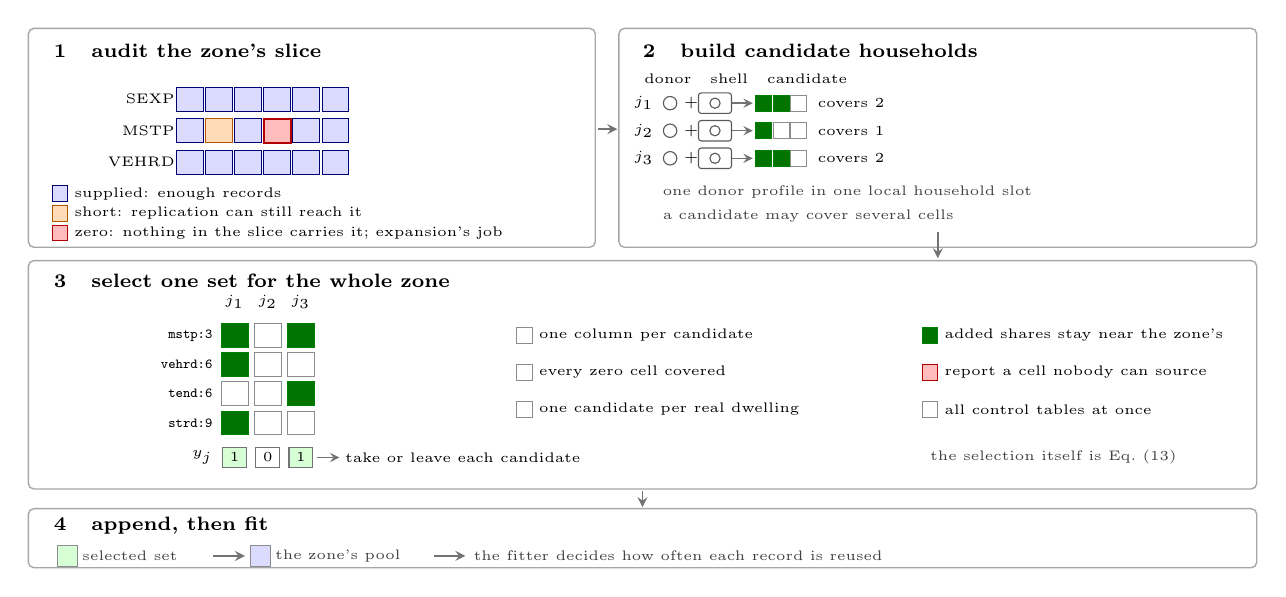
\begin{tikzpicture}[
  >=stealth,
  panel/.style={draw=black!35, rounded corners=2pt, line width=0.5pt},
  title/.style={font=\scriptsize\bfseries, anchor=west},
  cell/.style={draw=black!45, minimum width=0.34cm, minimum height=0.30cm,
               inner sep=0pt, line width=0.35pt},
  have/.style={cell, fill=blue!14, draw=blue!45!black},
  short/.style={cell, fill=orange!28, draw=orange!70!black},
  zero/.style={cell, fill=red!26, draw=red!70!black, line width=0.7pt},
  hit/.style={cell, fill=green!45!black, draw=green!50!black},
  rowlab/.style={font=\tiny, anchor=east, inner sep=1pt},
  collab/.style={font=\tiny, anchor=south, inner sep=1pt},
  tag/.style={font=\tiny, anchor=west, inner sep=0pt},
  note/.style={font=\tiny, align=left, text=black!75, inner sep=0pt},
  flow/.style={->, draw=black!55, line width=0.6pt},
  donor/.style={circle, draw=black!65, fill=white, minimum size=0.17cm,
                inner sep=0pt},
  shell/.style={draw=black!65, rounded corners=1pt, minimum width=0.42cm,
                minimum height=0.26cm, inner sep=0pt},
  xbox/.style={draw=black!55, minimum width=0.30cm, minimum height=0.26cm,
               inner sep=0pt, font=\tiny},
  small/.style={cell, minimum width=0.20cm, minimum height=0.20cm},
]

% ==================================================== 1  audit (top left)
\draw[panel] (0,1.12) rectangle (7.20,3.90);
\node[title] at (0.20,3.62) {1\quad audit the zone's slice};

\foreach \name/\y in {SEXP/3.00, MSTP/2.60, VEHRD/2.20} {
  \node[rowlab] at (1.90,\y) {\name};
}
% supplied everywhere except one short and one empty cell
\foreach \x in {2.05,2.42,2.79,3.16,3.53,3.90} {
  \node[have] at (\x,3.00) {};
  \node[have] at (\x,2.20) {};
}
\foreach \x/\state in {2.05/have,2.42/short,2.79/have,3.16/zero,
                       3.53/have,3.90/have} {
  \node[\state] at (\x,2.60) {};
}

% three-state legend, written as outcomes rather than as inequalities
\node[small, fill=blue!14, draw=blue!45!black] at (0.40,1.80) {};
\node[tag] at (0.58,1.80) {supplied: enough records};
\node[small, fill=orange!28, draw=orange!70!black] at (0.40,1.55) {};
\node[tag] at (0.58,1.55) {short: replication can still reach it};
\node[small, fill=red!26, draw=red!70!black] at (0.40,1.30) {};
\node[tag] at (0.58,1.30) {zero: nothing in the slice carries it;
  expansion's job};

% ============================================== 2  candidates (top right)
\draw[panel] (7.50,1.12) rectangle (15.60,3.90);
\node[title] at (7.68,3.62) {2\quad build candidate households};

\node[font=\tiny, anchor=west, inner sep=1pt] at (7.78,3.26) {donor};
\node[font=\tiny, anchor=west, inner sep=1pt] at (8.62,3.26) {shell};
\node[font=\tiny, anchor=west, inner sep=1pt] at (9.34,3.26) {candidate};

\foreach \y/\cov/\lab in {2.95/2/{$j_1$}, 2.60/1/{$j_2$}, 2.25/2/{$j_3$}} {
  \node[rowlab] at (7.98,\y) {\lab};
  \node[donor] at (8.15,\y) {};
  \node[font=\tiny] at (8.42,\y) {$+$};
  \node[shell] at (8.72,\y) {};
  \node[donor, minimum size=0.13cm] at (8.72,\y) {};
  \draw[flow, line width=0.5pt] (8.94,\y) -- (9.20,\y);
  \foreach \x in {9.34,9.56,9.78} {
    \node[cell, minimum width=0.20cm, minimum height=0.20cm] at (\x,\y) {};
  }
  \foreach \k in {1,...,\cov} {
    \node[hit, minimum width=0.20cm, minimum height=0.20cm]
      at ({9.34+(\k-1)*0.22},\y) {};
  }
  \node[tag] at (10.02,\y) {covers \cov};
}

\node[note, anchor=west] at (8.05,1.82)
  {one donor profile in one local household slot};
\node[note, anchor=west] at (8.05,1.52)
  {a candidate may cover several cells};

% ================================ 3  one selection for the zone (middle)
\draw[panel] (0,-1.95) rectangle (15.60,0.95);
\node[title] at (0.20,0.70) {3\quad select one set for the whole zone};

\foreach \x/\lab in {2.62/{$j_1$},3.04/{$j_2$},3.46/{$j_3$}} {
  \node[collab] at (\x,0.30) {\lab};
}
\foreach \name/\y in {\texttt{mstp:3}/0.00, \texttt{vehrd:6}/-0.37,
                     \texttt{tend:6}/-0.74, \texttt{strd:9}/-1.11} {
  \node[rowlab] at (2.38,\y) {\name};
}
\foreach \x in {2.62,3.04,3.46} {
  \foreach \y in {0.00,-0.37,-0.74,-1.11} {
    \node[cell] at (\x,\y) {};
  }
}
% j1 covers mstp, vehrd and strd; j3 covers mstp and tend; j2 is left out
\foreach \x/\y in {2.62/0.00,3.46/0.00,2.62/-0.37,3.46/-0.74,2.62/-1.11} {
  \node[hit] at (\x,\y) {};
}

\node[rowlab] at (2.38,-1.55) {$y_j$};
\node[xbox, fill=green!16] at (2.62,-1.55) {1};
\node[xbox] at (3.04,-1.55) {0};
\node[xbox, fill=green!16] at (3.46,-1.55) {1};
\draw[flow, line width=0.5pt] (3.66,-1.55) -- (3.95,-1.55);
\node[tag] at (4.02,-1.55) {take or leave each candidate};

% what the program enforces, in words
\node[small, fill=white, draw=black!45] at (6.30,0.00) {};
\node[tag] at (6.48,0.00) {one column per candidate};
\node[small, fill=white, draw=black!45] at (6.30,-0.47) {};
\node[tag] at (6.48,-0.47) {every zero cell covered};
\node[small, fill=white, draw=black!45] at (6.30,-0.94) {};
\node[tag] at (6.48,-0.94) {one candidate per real dwelling};
\node[small, fill=green!45!black, draw=green!50!black] at (11.45,0.00) {};
\node[tag] at (11.63,0.00) {added shares stay near the zone's};
\node[small, fill=red!26, draw=red!70!black] at (11.45,-0.47) {};
\node[tag] at (11.63,-0.47) {report a cell nobody can source};
\node[small] at (11.45,-0.94) {};
\node[tag] at (11.63,-0.94) {all control tables at once};
\node[note, anchor=west] at (11.45,-1.55)
  {the selection itself is Eq.~(13)};

% ============================================ 4  append, then fit (strip)
\draw[panel] (0,-2.95) rectangle (15.60,-2.20);
\node[title] at (0.20,-2.42) {4\quad append, then fit};

\node[cell, fill=green!16, minimum width=0.26cm, minimum height=0.26cm]
  at (0.50,-2.80) {};
\node[note, anchor=west] at (0.68,-2.80) {selected set};
\draw[flow] (2.35,-2.80) -- (2.75,-2.80);
\node[cell, fill=blue!14, minimum width=0.26cm, minimum height=0.26cm]
  at (2.95,-2.80) {};
\node[note, anchor=west] at (3.13,-2.80) {the zone's pool};
\draw[flow] (5.15,-2.80) -- (5.55,-2.80);
\node[note, anchor=west] at (5.65,-2.80)
  {the fitter decides how often each record is reused};


% ================================================================== arrows
\draw[flow] (7.23,2.62) -- (7.48,2.62);
\draw[flow] (11.55,1.32) -- (11.55,0.98);
\draw[flow] (7.80,-1.98) -- (7.80,-2.18);

\end{tikzpicture}
\caption{One zone through pool expansion. (1)~The zone's slice is audited cell by
cell; only a cell with no carrier at all is a pool defect, because a short cell can
still be reached by replication. (2)~A donor member profile is written into a slot of
a local shell household, giving one candidate that may cover several cells at once.
(3)~One binary choice per candidate, made for every control table together, must cover
the zero cells, keep the added shares near the zone's own, and report rather than
invent a cell that no candidate can source. (4)~The selected set is appended to the
zone's pool; how often a record is reused is decided by the fitter, not here.}
\label{fig:mip-expansion-process}
\end{figure}

\FloatBarrier
\subsection{Candidate-Pool Expansion: Demonstration}
\label{sec:pool_expansion_audit}

The two programs used by the candidate-pool expansion are Eqs.~\eqref{eq:mip_repair}
and~\eqref{eq:mip_joint} of Section~\ref{sec:mip_pool_expansion}: a per-candidate
repair that keeps as much of the real donor profile as the structural rules allow,
and a single binary selection program per zone that covers every sourceable
zero-capacity cell while keeping the added set's deviation from the zone's target
shares small. The released defaults are a 64-household and 256-person budget per
zone, coverage weight $\lambda_0=10^{5}$ and marginal weight $\lambda_1=10^{-2}$;
over the 256-person budget the whole marginal term stays below about
$2.6\times10^{4}$, so opening a sourceable cell always outranks any marginal gain
the added set could buy. Coverage is soft through the slack $e_c$, so a cell that no
donor can source is reported rather than making the program infeasible.

Table~\ref{tab:pool_expansion_audit} reports the ten-zone demonstration. The
demonstration is a mechanism check on a subset of zones under one fixed set of
parameters; it establishes that the step can fill the sourceable zero cells with a
small number of feasible records, not that it closes any zone's full deficit, which
is a question for the zone fit and the validation tables. Of 123 zero-capacity
cells, 70 of the 73 sourceable cells received a feasible candidate and all 70 were
covered, with 14 households (18 persons) selected in total and every selection
program solving to optimality. The weighted marginal deviation of the \emph{added
set} ranged from 0.239 to 1.622 (median 0.406); because each zone's addition is only
one to three persons, a single person can move a cell share substantially, so this
figure describes the added set, not the fitted zone population. The 53 uncovered
cells split into 40 in four categories absent from the census extract, ten in a
padding code, and three for which no donor--shell candidate survived the household
and rule checks---the first fifty are treated by the current parameters as absent or
padding, and the last three identify a candidate-generation gap rather than a
structural zero.

\begin{table}[h!]
\centering
\caption{Ten-zone demonstration of candidate-pool expansion. \emph{Zero} is the
number of positive-target control cells with zero attainable capacity;
\emph{Cov.} the number covered by the selected set; \emph{HH} and \emph{Persons}
the added records; \emph{Dev.} the weighted marginal deviation of the added set
(lower is better). All ten selection programs returned an optimal solution. The
53 uncovered cells are 40 in census-absent codes, ten in a padding code, and
three with no feasible donor--shell candidate.}
\label{tab:pool_expansion_audit}
\small
\begin{tabular}{@{}lrrrrr@{}}
\toprule
Zone & Zero & Cov. & HH & Persons & Dev. \\
\midrule
112011236 & 13 & 8 & 2 & 3 & 1.113 \\
112011237 & 13 & 7 & 2 & 2 & 0.239 \\
112011238 & 11 & 6 & 1 & 1 & 0.458 \\
112011239 & 12 & 7 & 1 & 1 & 0.309 \\
112011240 & 13 & 8 & 2 & 3 & 0.355 \\
112011241 & 11 & 6 & 1 & 1 & 0.341 \\
112011242 & 13 & 7 & 1 & 1 & 0.827 \\
112011243 & 12 & 7 & 1 & 1 & 0.772 \\
112021244 & 13 & 8 & 2 & 3 & 1.622 \\
112021245 & 12 & 6 & 1 & 2 & 0.288 \\
\midrule
Total  & 123 & 70 & 14 & 18 & 6.326 \\
Median & 12  & 7  & 1  & 1  & 0.406 \\
\bottomrule
\end{tabular}
\end{table}
\FloatBarrier

\input{files/repair_appendix.tex}



\subsection{Computation Settings}
The settings shared by every SA strategy are listed in \cref{tab:sa_settings}.
\begin{table}[H]
\centering
\small
\caption{Simulated-annealing settings shared by every SA strategy.}
\label{tab:sa_settings}
\begin{tabular}{@{}p{0.24\textwidth}p{0.66\textwidth}@{}}
\toprule
\textbf{Parameter} & \textbf{Setting} \\
\midrule
Iterations per zone & 1{,}000 \\
Initial temperature & auto-calibrated to the measured cost scale (about $10^{-4}$) \\
Cooling rate $\alpha$ & 0.95; 0.995 when 0.95 would cool too aggressively \\
Move types & household add/remove/swap; constraint-safe attribute relabelling; \ family dwelling-attribute mutation (VEHRD, STRD) \\
Acceptance rule & Metropolis, $\exp(-\Delta\text{RSSZ}/T)$ \\
Convergence tolerance & $\text{tol}_{k,m}=0.05$, a reporting threshold only; not part of the acceptance rule \\
Retained solution & best-so-far only; the current solution may move uphill \\
\bottomrule
\end{tabular}
\end{table}


\end{document}